\documentclass[twoside,a4paper,11pt]{book}
\usepackage[twoside,a4paper,top=25mm,bottom=25mm,left=20mm,right=20mm]{geometry}

\usepackage{float}
%\usepackage{graphics}
\usepackage[dvips]{epsfig,rotating}

\usepackage{verbatim}
\usepackage{amsmath}
\usepackage{amssymb}

%\usepackage{html}

% Table Settings
\usepackage{longtable}
\usepackage[table]{xcolor}
\usepackage{tabu}
\usepackage{multirow}
\usepackage{tabularx}
% \usepackage{makecell}
\tabulinesep=^1mm_1mm
\renewcommand{\arraystretch}{1.1}

\usepackage{caption}
\captionsetup[table]{skip=2pt}

\usepackage{todonotes}
%\usepackage{draftwatermark}

\usepackage{fancyvrb}

% Colours
\definecolor{cverbbg}{gray}{0.95}
\definecolor{cverbbd}{gray}{0.35}
\definecolor{notered}{rgb}{0.70,0.0,0.0}
\definecolor{linkred}{rgb}{0.70,0.1,0.0}

% Links
\usepackage{hyperref}
\usepackage{url}
\hypersetup{colorlinks=true, citecolor=blue, urlcolor=blue, linkcolor=linkred}
\urlstyle{same}

% Index
\usepackage{makeidx}
\makeindex

% Verbatim Box
\newenvironment{cverbatim}
 {\SaveVerbatim{cverb}}
 {\endSaveVerbatim
  \scriptsize\flushleft\addtolength{\leftskip}{5mm}
  \fboxrule=0.4pt\fboxsep=0.6em
  \fcolorbox{cverbbd}{cverbbg}{\BUseVerbatim{cverb}}%
  \endflushleft\normalsize
}

\newenvironment{ctverbatim}
 {\SaveVerbatim{ctverb}}
 {\endSaveVerbatim
  \tiny\flushleft\addtolength{\leftskip}{5mm}
  \fboxrule=0.4pt\fboxsep=0.6em
  \fcolorbox{cverbbd}{cverbbg}{\BUseVerbatim{ctverb}}%
  \endflushleft\normalsize
}

\setcounter{secnumdepth}{3}
\setcounter{tocdepth}{3}
\pagestyle{headings}
\raggedbottom

% Page Layout
%*************

\usepackage{fancyhdr}

% Plain Page Numbering
\fancypagestyle{plain}{
    \fancyhf{}
    \fancyfoot[LE,RO]{\thepage}
}

% Header style for numbered chapters
\newcommand{\defaulthead}{
    \fancyhead[LE]{\nouppercase{\scshape\leftmark}}
    \fancyhead[RO]{\nouppercase{\scshape\rightmark}}
}

% Custom heading for unnumbered chapters
\newcommand{\simplehead}[1]{
    \fancyhead[LE]{\nouppercase{\itshape #1}}
    \fancyhead[RO]{\nouppercase{\itshape #1}}
}

\pagestyle{fancy}

% Page Header
\renewcommand{\chaptermark}[1]{\markboth{\chaptername\ \thechapter: #1}{}}
\renewcommand{\sectionmark}[1]{\markright{\thesection\ #1}{}}
\renewcommand{\headrulewidth}{0pt}
\renewcommand{\footrulewidth}{0pt}

\fancyhf{}
\defaulthead
\headheight 15pt
\fancyfoot[LE,RO]{\thepage}

% Main Document
\begin{document}

\frontmatter
\pagenumbering{roman}

\pdfbookmark{Title Page}{TitlePage}
\begin{titlepage}
\begin{center}\normalsize\scshape
    European Organization for Nuclear Research \\
    CERN BE/ABP
\end{center}
\vspace*{2mm}
\begin{flushright}
    CERN/SL/94-56 \\
    Updated May 2019
\end{flushright}
\begin{center}\Huge
    \textbf{SixTrack} \\
    \LARGE Version 5.2.6 \\
    \vspace*{8mm}Single Particle Tracking Code Treating Transverse Motion with Synchrotron Oscillations in a Symplectic Manner \\
    \vspace*{8mm}\textbf{User's Reference Manual}
\end{center}
\begin{center}
    F. Schmidt,
    A.~Alekou,
    V.K.~Berglyd~Olsen,
    R.~De~Maria,
    M.~Fitterer,
    S.~Kostoglou,\\
    A.~Mereghetti,
    T.~Persson,
    K.~Sjobak,
    J.F.~Wagner,
    and
    S.J.~Wretborn,
\end{center}
\begin{center}\large
    \vspace*{10mm}\textbf{Abstract} \\
\end{center}
The aim of SixTrack is to track two nearby particles taking into account the full six--dimensional phase space including synchrotron oscillations in a symplectic manner.
It allows to predict the long--term dynamic aperture which is defined as the border between regular and chaotic motion.
This border can be found by studying the evolution of the distance in phase space of two initially nearby particles.
Parameters of interest like nonlinear detuning and smear are determined via a post processing of the tracking data.
An analysis of the first order resonances can be done and correction schemes for several of those resonances can be calculated.
Moreover, there is the feature to calculate a one--turn map to very high order and the full six--dimensional case, using LBL differential algebra.
This map allows a subsequent theoretical analysis like normal form procedures which are provided by \'{E}. Forest~\cite{DALIE}.

The linear elements are usually treated as thick elements in SixTrack\@.
In that case there is at least one non--zero length element in the structure file which is not a drift element.
If the accelerator, however, is modelled exclusively with drifts and kicks, SixTrack automatically uses the thin lens formalism according to G.~Ripken \cite{Ripken95}.
A common header of output data and the format of these data has been found for MAD and SixTrack tracking data.

\vfill
\begin{center}
    Geneva, Switzerland \\
    \today
\end{center}

\end{titlepage}

\cleardoublepage

\pdfbookmark{Acknowledgements}{Acknowledgements}
\chapter*{Acknowledgement}

I would like to thank my colleagues at DESY and CERN to help to find nasty bugs and for a thorough check of the program.
I would like to thank Mikko Vaenttinen who helped to vectorise the program.
He also did most of the typing of the manuscript.
Moreover, I want to express my gratitude to F.~Zimmermann who helped to finish the differential--algebra part in endless night sessions.
Additions concerning Normal Forms have been contributed by M.~Giovannozzi.
J.~Miles helped with the calculation of the 6D Courant--Snyder matrix and its use to transform the tracking data in the post--processing.
W.~Herr is thanked for providing a software package used for the orbit correction. L.H.A.~Leunissen extracted and adapted the 6D beam--beam code of Hirata~\cite{Hirata}.

\bigskip
\begin{flushright}
    -- \textit{F. Schmidt, for the version 3.x and 4.x manual}
\end{flushright}

\cleardoublepage

\pdfbookmark{Contents}{Contents}
\tableofcontents
\cleardoublepage
\pagenumbering{arabic}

% Chapters
\mainmatter

\chapter{Introduction} \label{Intro}

The Single Particle Tracking Code SixTrack is optimised to carry two particles~\footnote{Two particles are needed for the detection of  chaotic behaviour.} through an accelerator structure over a large number of turns.
It is an offspring of RACETRACK~\cite{RACETRACK}\index{RACETRACK} written by Albin Wrulich.
The input structure has been changed as little as possible so that slightly modified RACETRACK input files, or those of other offsprings like FASTRAC \cite{FASTRAC} can be read.

\paragraph{The main features of SixTrack are:}~
\begin{enumerate}
    \item Treatment of the full six-dimensional motion including synchrotron motion in a symplectic manner \cite{Ripken85}. The energy can be ramped at the same time considering the relativistic change of the velocity \cite{Ripken87}.
    \item Detection of the onset of chaotic motion and thereby the long term dynamic aperture by evaluating the Lyapunov exponent.
    \item Post processing procedure allowing:
    \begin{itemize}
        \item calculation of the Lyapunov exponent,
        \item calculation of the average phase advance per turn,
        \item FFT analysis,
        \item resonance analysis,
        \item calculation of the average, maximum and minimum values of the Courant-Snyder emittance and the invariants of linearly coupled motion,
        \item calculation of smear, and
        \item plotting using the CERN packages HBOOK, HPLOT and HIGZ \cite{HBOOK,HPLOT,HIGZ}
    \end{itemize}
    \item Calculation of first order resonances and of correction schemes for the resonances \cite{Gilbert78}.
    \item Calculation of the one turn map using the differential algebra techniques. The original DA package by M.Berz \cite{Berz89} has been replaced by the package of LBL~\cite{DALIE}. The Fortran code is transferred into a Map producing via the (slightly modified) ``DAFOR'' code~\cite{DAFOR}.
    \item The code is vectorised, with two particles, the number of amplitudes, the different relative momentum deviations $\Delta p/p_0$ in parallel \cite{Sixvec}.
    \item Operational improvements:
    \begin{itemize}
        \item free format input,
        \item optimisation of the calculation of multipole kicks,
        \item improved treatment of random errors,
        \item each binary data file has a header describing the history of the run (Appendix~\ref{Header})
    \end{itemize}
\end{enumerate}

% ================================================================================================================================ %
\section{Versions and Service}

There are two versions: for element by element tracking there is a vector version, and there is a version to produce a one turn map using the LBL Differential Algebra package.
In both cases the input structure file\index{structure file} \texttt{fort.2}\index{fort.2} is used to determine if the thick or thin linear element mode has to be used.

To use the power of the Differential Algebra\index{SixDA}, for instance to calculate the 6D closed orbit in an elegant fashion, the tracking versions may also be equipped with a low order map facility to avoid the otherwise huge demand on memory.

It must be mentioned that in the linear thin lens version dipoles have to be treated in a special way.
See section~\ref{MulBlo} for details.

To convert MAD-X files into SixTrack input, a special conversion program $mad\_6t$~\cite{CONVERTOR} has been developed (see also~\ref{MADT}).

The following subroutines are taken from various packages:

\begin{table}[h]
    \caption{External Routines}
    \label{T-ExtRou}
    \centering
    \renewcommand{\arraystretch}{1.5}
    \begin{tabular}{|l|l|l|}
        \hline
        \rowcolor{blue!30}
        \textbf{Package} & \textbf{Routine} & \textbf{Purpose} \\
        \hline
        \texttt{HBOOK}  & \texttt{HBOOK2, HDELET, HLIMIT, HTITLE} & Graphic basics \\
        \hline
        \texttt{HPLOT}  & \texttt{HPLAX,  HPLCAP, HPLEND, HPLINT} & Graphic options \\
        \cline{2-2}
                        & \texttt{HPLOPT, HPLSET, HPLSIZ, HPLSOF} &  \\
        \hline
        \texttt{HIGZ}   & \texttt{IGMETA, ISELNT, IPM, IPL}       & Graphic output \\
        \hline
    \end{tabular}
\end{table}

All versions can be downloaded from the web.
The project webpage is found at \url{http://sixtrack.web.cern.ch/},
  and primary source repository is located at \url{https://github.com/SixTrack/SixTrack}.
Older versions can be found at \url{http://cern.ch/Frank.Schmidt/Source}.

In case of problems, please see the CERN SixTrack egroups ``sixtrack-users'' and ``sixtrack-developers''.
If these are not accessible to you, you are welcome to contact the coordinators: Riccardo De Maria and Kyrre Sjobak, as well as the original developer Frank Schmidt.
Our contact details are available from the CERN phonebook.

If you think you have found a defect in the program, please create a report on the issue tracker\index{SixTrack bug reports} at \url{https://github.com/SixTrack/SixTrack/issues}.
Note that for this to be usefull, you need to describe what the program is doing, what you expected it to do, and an example which demonstrates the unwanted behaviour.
Plase also look through the issues that are already listed, and see if it has already been reported.
If so, you are welcome to add a comment to the issue, which may influence its priority and give additional and useful information to the developers.

The most up to date version of the documentation can always be found on the GitHub repository mentioned above.\index{SixTrack source}
Additionally, various older documentation can be found at \url{http://cern.ch/Frank.Schmidt/Documentation/doc.html}.

% ================================================================================================================================ %
\section{Evolution of SixTrack}

Following, is a short historical overview of how the versions of SixTrack have evolved.
\begin{itemize}
    \item \textbf{Version 1}
        The first version has been an upgrade of RACETRACK~\cite{RACETRACK} to include the full 6D formalism for long linear elements by G.~Ripken~\cite{Ripken85}.
    \item \textbf{Version 2}
        The DA package and the Normal Form techniques~\cite{Berz89,Forest89} have been added to allow the production of high order one turn Taylor maps and their analysis.
        The 6D thin lens formalism~\cite{Ripken95} has also been included to speed up the tracking without appreciable deterioration of the accelerator model for very large Hadron colliders like the LHC.
    \item \textbf{Version 3}
        The beam--beam kick \`a la Bassetti and Erskine~\cite{BasErs} has been included together with the 6D part by Hirata et al.~\cite{Hirata}.
        Moreover, this 6D part has been upgraded to include the full 6D linear coupling~\cite{ripbeam}.
        Lastly, the LBL DA package has replaced the original one by Berz, and all operations needed to set up the accelerator structure are now performed with the help of Forest's LieLib package~\cite{DALIE}.
    \item \textbf{Version 4}
        \todo[inline]{Add stuff}
    \item \textbf{Version 5}
        Machine size and particle numbers are no longer defined by compiler flags but allocated dynamically based on the input files.
        Merges the Collimation version of SixTrack into the main code.
        Code-wide implementation of rounding of input float values from text, as well as output of float values to text in critical parts, provided by the CRLIBM library.
        This also includes a wrapper for consistent rounding of values from mathematical functions.
        Adds experimental support for HDF5 and ROOT output files.
        Extensive rewrite of many sections of the code to increase flexibility and modularity, as well as bug fixes to the physics.
        Includes a full rewrite of the input parsing and upgrade of the source to Fortran 2008.
        Support for 32, 64 and 128 bit floating point precision.
        Replaces the astuce preprocessor with the c preprocessor.
\end{itemize}

For a more detailed list of changes, see \texttt{CHANGELOG.md} in the repository.

% Formerly in Chapter: Conclusions
Programs with large input structures like SixTrack tend to be far from perfect, even though a cumbersome chase for program bugs and a lot of polishing on the input structure has been performed.
Plenty of comments and suggestions are therefore needed to further improve the program.

% ================================================================================================================================ %
\section{SixTrack Input Structure}

The SixTrack input is line oriented.\index{SixTrack input}\index{fort.3}
Each line is treated as one string of input in which a certain sequence of numbers and character strings is expected to be found.
The numbers and character strings must be separated by at least one blank space.
Floating point numbers can be given in any format, but must be distinguishable from integer numbers.
Comments can be added starting with the character ``!''.\index{comment lines}
Empty lines and lines starting with the comment character will be ignored and are not counted towards the line number requirement that apply to many of the input blocks.
For beckwards compatibility, lines starting with a slash ``/'' in the first column will also be ignored by the program.

For detailed questions concerning rounding errors, calculation of the Lyapunov exponent and determination of the long term dynamic aperture, see \cite{thesis}.\index{rounding errors}

% ================================================================================================================================ %
\subsection{Input Format} \label{sec:informat}

The input format used in SixTrack has been inherited from RACETRACK.
This system makes it easy to read input and allows easy change and addition of input blocks.

The idea of the input format is to use a sequence of input blocks, each block with a specific keyword in the first line.\index{input blocks}
The block is terminated by the keyword \texttt{NEXT} in the last line.\index{NEXT}
The input data goes in the lines in between.
The keyword \texttt{ENDE} ends the input sequence, and anything after this keyword is ignored.\index{ENDE}
This system makes it easy to read input and allows easy change and addition of input blocks.
Values inside a block can be indented, but the opening ang closing keywords cannot.
In some blocks more than 4 space indentation signify a line continuation of the previous line.
It is therefore advisable to keep indentation at less than 5 spaces to avoid unpredictable results.

From version 5, SixTrack enforces the proper closing of input blocks, which in the past have been somewhat inconsistent.
This does not apply to the first line, which contains the flag to determine which file to read the lattice from.
If a \texttt{NEXT} keyword is added after this, an error is raised.
Multiple occurences of the same input block is, as a general rule, not allowed and will cause an error.
However, there are a few exceptions.
String input variables can be wrapped in either single or double quotes.
SixTrack will also accept strings without quotes, provided they do not contain tabs, spaces or the comment character.

Input errors will provide a descriptive error message, the line number and file in which the error was encountered, and a printout of the line where the error was found.
A new \texttt{SETTINGS} block has been added in SixTrack 5 where a \texttt{DEBUG} flag can be added.\index{DEBUG}
When this flag is set, most values read from the file will be printed back with the value it was converted to internally in SixTrack, and if it was modified, what it was changed to.

In the following chapters, the input structure of SixTrack is discussed in detail.
To facilitate the use of the program, a list of default values in Appendix~\ref{Default}, the input and output files are described in Appendix~\ref{Files}, and a description of the data structure of the binary data files in Appendix~\ref{Header}.

% ================================================================================================================================ %
\subsection{Input Values} \label{sec:invals}

\paragraph{Integers} must be entered as plain integers.
\paragraph{Floats} can be entered as integers (converted during parsing) and standard Fortran floats.\\
Examples \texttt{1, 1.0, 1.0e3, 1e3, 1.0d3, 1d3, 1.0q3, 1q3}.
\paragraph{Strings} can be entered with both single and double quotes, and without quotes if the string contains no spaces or comment characters.
\paragraph{Flags} accept the following entries: \texttt{.true./.false.}, \texttt{true/false}, \texttt{yes/no}, \texttt{on/off}, and \texttt{1/0}. These are not case sensitive.

% ================================================================================================================================ %
\subsection{Command Line Arguments} \label{sec:cmdarg}

SixTrack does not require any command line arguments, but can optionally take the file name for the main input file as well as the geometry file as the first and second argument, respectively.
See also Sections~\ref{InFiles} and~\ref{ProVer}.

\bigskip
\noindent In addition, SixTrack can echo the version number and exit with the following flags:
\begin{itemize}
    \item[\texttt{-v}] Echo program name and version as a single line, and exit.
    \item[\texttt{-V}] Echo program name, version, release date, and git hash on four lines, and exit.
    \item[\texttt{-nv}] Echo the numerical version as an integer, and exit,
\end{itemize}

\cleardoublepage

\chapter{General Input} \label{GenInp}

% ================================================================================================================================ %
\section{Main Input Files} \label{InFiles}

SixTrack requires a main input file, which by default must be named \texttt{fort.3}.
Alternatively, if a different file name is needed, it can be given to the SixTrack executable as the first command line argument.
If a geometry file is requested in the main input file (see Section~\ref{ProVer}), it can be given as the second command line argument.
If none is provided, SixTrack will look for a file named \texttt{fort.2}.
These files will be referred to as \texttt{fort.3} and \texttt{fort.2} in the rest of this document.

\bigskip
Note that you can always add the global \texttt{DEBUG} flag to the \texttt{SETTINGS} block to enable echoing back most of the input parameters set in the \texttt{fort.3} file.
The flag is described in Section~\ref{STSett}.
This can not only verify that SixTrack understood and received the values correctly, but it also often echoes back other parameters computed from the input values.
The echoed back lines will start with ``\texttt{INPUT> DEBUG}'', so it is sometimes easier to grep for these lines in the output.
They contain the nme of the block where they were parsed, and the line number within the block if available.

% ================================================================================================================================ %
\section{Program Version} \label{ProVer}

The \textit{Program Version} input block determines if all of the input will be in the input file \texttt{fort.3}, or if the geometry part of the machine (see~\ref{MaGe}) will be in a separate file: \texttt{fort.2}.\index{input block}\index{fort.2}\index{fort.3}
The latter option is useful if tracking parameters are changed, but the geometry part of the input is left as it is.
The geometry part can be produced directly from a MAD-X input file (see~\ref{MADT}).
Note that this line should not have a \texttt{NEXT} keyword after it.\index{NEXT}

\bigskip
\begin{tabular}{@{}lp{0.8\linewidth}}
    \textbf{Keyword}    & \texttt{FREE} or \texttt{GEOM} \index{FREE}\index{GEOM}\\
    \textbf{Data lines} & None \\
    \textbf{Format}     & \texttt{keyword comment title} \\
\end{tabular}

\paragraph{Format Description}~

\bigskip
\begin{tabular}{@{}lp{0.8\linewidth}}
    \texttt{keyword} & The first four characters of the first line of the \texttt{fort.3} input file are reserved for the keyword. \texttt{FREE} for free format input with all input in \texttt{fort.3}, and \texttt{GEOM} if the geometry part is in file  \texttt{fort.2}. \\
    \texttt{comment} & Following the first four characters, 8 characters are reserved for comments \\
    \texttt{title}   & The next 60 characters are interpreted as the title printed at the top of the output file \texttt{fort.6}.
\end{tabular}

% ================================================================================================================================ %
\section{Print Selection} \label{PriSel}

The \texttt{PRIN} flag is deprecated, and replaced by the \texttt{PRINT} flag in the \texttt{SETTINGS} block.\index{PRIN}

% ================================================================================================================================ %
\section{Settings} \label{STSett}

The \textit{Print Selection} input block available in earlier version has been replaced with the \texttt{SETTINGS} block.\index{SETT}
This was done to allow for more options related to what output SixTrack produces in \texttt{fort.6}.\index{fort.6}
The \texttt{PRIN} flag is available as one of several options in this block.\index{PRIN}
However, for backwards compatibility, the \texttt{PRIN} flag is still accepted.

\bigskip
\begin{tabular}{@{}lp{0.8\linewidth}}
    \textbf{Keyword}    & \texttt{SETT} \\
    \textbf{Data lines} & Variable
\end{tabular}

\paragraph{Format Description}~

\bigskip
\begin{tabular}{@{}lp{0.8\linewidth}}
    \texttt{PRINT} & This causes the printing of the input data to the output file \texttt{fort.6}. \\
    \texttt{DEBUG} & A global debug flag that causes the majority of the blocks to echo back the value read from the input file after parsing. It may also print out secondary values set based on input values read, or modification made to input values based on other dependencies and criteria.\index{DEBUG}\\
    \texttt{QUIET} & Followed by an integer specifying how ``quiet'' the output should be. A higher value causes less information to be printed back out. If the keyword is not present, the default value is 0, which means it is disabled. If it is present, but the integer value is omitted, it is set to be 1. This flag does not interfere with the \texttt{PRINT} flag.\index{QUIET}\\
    \texttt{PRINT\_DCUM} & This will cause the calculated s-coordinate of each structure element to be printed to the file \texttt{machine\_length.dat}. \\
    \texttt{PARTSUMMARY} & Enable or disable the printing of a particle summary after tracking. The flag takes an optional parameter to explicitly state whether it is ON or OFF. If omitted, it is assumed the user requests it to be ON. If the flag is omitted entirely, the default behaviour is determined by the particle count. If SixTrack is running with 64 particles or less, it is ON by default, otherwise OFF.\index{particle summary}\\
    \texttt{WRITEFORT12} & Enable or disable the writing of \texttt{fort.12} after tracking. The flag takes an optional parameter to explicitly state whether it is ON or OFF. If omitted, it is assumed the user requests it to be ON. If the flag is omitted entirely, the default behaviour is determined by the particle count. If SixTrack is running with 64 particles or less, it is ON by default, otherwise OFF.\index{fort.12}\\
    \texttt{INITIALSTATE} & Followed by either ``binary'' or ``text''. This will write a file before tracking containing the initial state of all particles to either a binary or a text file.\index{initial state} Adding ``ions'' as a second keyword will also dump the additional ion columns (see Section~\ref{hions}). The file header also contains the settings of the reference particle, the 4D and 6D closed orbit, the tunes, and the TA matrix. (Note that the $\mbox{d}p/p_0$ values are not scaled by a factor 1000 in this file.)\index{TA Matrix} \\
    \texttt{FINALSTATE} & Followed by either ``binary'' or ``text''. This will write a file after tracking containing the final state of all particles, including those lost during tracking, to either a binary or a text file.\index{final state} Adding ``ions'' as a second keyword will also dump the additional ion columns (see Section~\ref{hions}). The file header also contains the settings of the reference particle, the 4D and 6D closed orbit, and the TA matrix. (Note that the $\mbox{d}p/p_0$ values are not scaled by a factor 1000 in this file.)\index{TA Matrix} \\
\end{tabular}


% ================================================================================================================================ %
\section{Comment Line} \label{ComLin}

An additional comment can be specified with the \textit{Comment} block.
The comment will be written to the binary data files (Appendix~\ref{Header}), and will appear in the post processing output as well.

\bigskip
\begin{tabular}{@{}lp{0.8\linewidth}}
    \textbf{Keyword}    & \texttt{COMM}\index{COMM}\index{comment} \\
    \textbf{Data lines} & 1 \\
    \textbf{Format}     & A string of up to 80 characters.
\end{tabular}

% ================================================================================================================================ %
\section{Iteration Errors} \label{IteErr}

For the processing procedures, the number of iterations and the precision to which the processing is to be performed are chosen with the \textit{Iteration Errors} input block.\index{iteration errors}
If the input block is left out, default values will be used.

\bigskip
\begin{tabular}{@{}lp{0.8\linewidth}}
    \textbf{Keyword}    & \texttt{ITER}\index{ITER} \\
    \textbf{Data lines} & 1 to 4 \\
    \textbf{Format}     & Each data line holds three values as in table~\ref{T-IteErr}, except for the fourth line where the horizontal and vertical aperture limits can be additionally specified. This has been added to avoid artificial crashes for special machines.
\end{tabular}

\begin{table}[h]
    \caption{Iteration Errors\index{chromaticity}\index{dispersion}\index{aperture limit}\index{closed orbit}}
    \label{T-IteErr}
    % \footnotesize
    \centering
    \renewcommand{\arraystretch}{1.5}
    \begin{tabular}{|l|l|l|>{\raggedright\arraybackslash}p{10.2cm}|}
        \hline
        \rowcolor{blue!30}
        \textbf{Variable} & \textbf{Type} & \textbf{Default} & \textbf{Description} \\
        \rowcolor{gray!15}
        \multicolumn{4}{|l|}{Data Line 1} \\
        \hline
        \texttt{ITCO} & \texttt{int} & \texttt{50}    & Number of Iterations for closed orbit calculation. \\
        \hline
        \texttt{DMA}  & \texttt{dbl} & \texttt{1e-12} & Demanded Precision of closed orbit displacements. \\
        \hline
        \texttt{DMAP} & \texttt{dbl} & \texttt{1e-15} & Demanded Precision of derivative of closed orbit displacements. \\
        \hline
        \rowcolor{gray!15}
        \multicolumn{4}{|l|}{Data Line 2} \\
        \hline
        \texttt{ITQV} & \texttt{int} & \texttt{10}    & Number of Iterations for Q Adjustment. \\
        \hline
        \texttt{DKQ}  & \texttt{dbl} & \texttt{1e-10} & Variations of quadrupole strengths. \\
        \hline
        \texttt{DQQ}  & \texttt{dbl} & \texttt{1e-10} & Demanded Precision of tunes. \\
        \hline
        \rowcolor{gray!15}
        \multicolumn{4}{|l|}{Data Line 3} \\
        \hline
        \texttt{ITCRO} & \texttt{int} & \texttt{10}    & Number of Iterations for chromaticity correction. \\
        \hline
        \texttt{DSM0}  & \texttt{dbl} & \texttt{1e-10} & Variations of sextupole strengths. \\
        \hline
        \texttt{DECH}  & \texttt{dbl} & \texttt{1e-10} & Demanded Precision of chromaticity correction. \\
        \hline
        \rowcolor{gray!15}
        \multicolumn{4}{|l|}{Data Line 4} \\
        \hline
        \texttt{DE0} & \texttt{dbl} & \texttt{1e-9} & Variations of momentum spread for chromaticity calculation. \\
        \hline
        \texttt{DED} & \texttt{dbl} & \texttt{1e-9} & Variations of momentum spread for evaluation of dispersion. \\
        \hline
        \texttt{DSI} & \texttt{dbl} & \texttt{1e-9} & Demanded Precision of desired orbit r.m.s. value; compensation of resonance width. \\
        \hline
        \texttt{APER(1)} & \texttt{dbl} & \texttt{1000 [mm]} & Demanded Precision of horizontal aperture limit. \\
        \hline
        \texttt{APER(2)} & \texttt{dbl} & \texttt{1000 [mm]} & Demanded Precision of vertical aperture limit. \\
        \hline
    \end{tabular}
    % \normalsize
\end{table}

% ================================================================================================================================ %
\section{MAD-X to SixTrack Conversion} \label{MADT}

A converter has been developed~\cite{CONVERTOR}, which is directly linked to MAD-X\@.\index{MAD-X}
It produces the geometry file \texttt{fort.2}; an appendix to the parameter file \texttt{fort.3}, which defines which of the multipole errors are switched on; the error file \texttt{fort.16}, and the file \texttt{fort.8} which holds the transverse misalignments and the tilt of the non-linear kick elements.\index{fort.8}\index{fort.16}\index{multipole errors}
It also produce a file \texttt{fort.34} with linear lattice functions, phase advances and multipole strengths needed for resonance calculations for the program \textit{SODD}~\cite{SODD}.\index{fort.34}\index{resonance calculations}

In addition, the flag \texttt{aperture} will produce an aperture limitations file.
The flag \texttt{multicol} will produce an alternative \texttt{fort.2} file with more information on the machine structure (see Section~\ref{stru:multicol}).

% A description of %how to use the converter can be found in Appendix\ref{MADSIXC}.
% Pasted here for reference:

% \chapter{MAD SixTrack Convertor} \label{MADSIXC}

% A special version of the MAD program has been generated that creates
% input files for SixTrack with the complete and exact description of
% the current accelerator model stored in MAD\@. This then allows a
% detailed comparison of the tracking results from both programs.

% The programs SixTrack and MAD \cite {MAD} are both used for particle
% tracking in realistic machines such as the LHC with all expected field
% errors up to the highest order, and with displacement errors of
% quadrupoles and possibly other elements. The LHC lattice and error
% description, however, exists only in MAD format due to its much
% greater flexibility and readability. If one wants to compare tracking
% results of the two programs one needs therefore a conversion of the
% current machine inside MAD into SixTrack format. In particular the
% generated random field and displacement errors have to be transmitted
% correctly since they influence the outcome of the long-term tracking
% greatly.

% To this end it was necessary to make a special MAD version that reads
% a machine description, expands it, generates the errors, and then
% performs the necessary transformations for SixTrack: different
% conventions for the signs of magnet forces, grouping of identical
% elements, concatenation of multiple drift spaces, creation of blocks
% of linear elements between nonlinear ones, a different description
% of field and position errors, and similar tedious questions had to be
% solved. The results of the transformation are then written into input
% files for SixTrack.

% The special MAD version is actually a full MAD (except for plotting)
% with an additional module for the SixTrack output.  This then allows
% the user to perform orbit corrections and other calculations inside
% MAD, and have the resulting modifications of the machine be
% transferred to SixTrack.  All position errors (including tilt errors)
% and field errors are transmitted.

% The converter works correctly for thin and thick lens lattices.  In
% the latter case, all dipoles and quadrupoles are split into two, and a
% multipole is inserted in the centre, except for orbit corrector
% magnets which are converted to thin lens.  Since MAD does not support
% field errors higher than third order for thick elements, the
% multipolar errors will have to be created with the corresponding thin
% lens model, or by some other means.

% The special MAD version accepts one additional command:
% \begin{verbatim}
%  sixt:
%       elem       = (up to 20) element names
%       lgelem     = (up to 20) lengths of the above elements
%       structure  = structure file name, default: "fort.2"
%       param_in   = name of a (mandatory, possibly empty)
%                    extra input file for MAD, default: "fort.3.in"
%       param_out  = parameter file name, default: "fort.3"
%       errors     = field errors file name, default: "fort.16"
%       poserr     = position errors file name, default: "fort.8"
%       cavall     = all cavities in the structure, default: one only.
% \end{verbatim}
% The element length facility is necessary to give SixTrack the real
% lengths of the dipoles (and possibly other elements) that are replaced
% by thin multipoles.  \\
% The parameter input file is copied to the start of the parameter
% output file which may be useful in certain situations.

\cleardoublepage

\chapter{Initial Conditions for Tracking} \label{InitCondTrack}

For the study of non-linear systems, the choice of initial conditions is of crucial importance.\index{initial conditions}
The input structure for the initial conditions was therefore organised in such a way as to allow for maximum flexibility.
SixTrack is optimised to reach the largest possible number of turns.
In order to derive the Lyapunov exponent\index{Lyapunov exponent}, and thereby to distinguish between regular and chaotic motion, the particle has a close by companion particle.
Moreover, experience has shown that varying only the amplitude while keeping the phases constant is sufficient to understand the non-linear dynamics, as a subsequent detailed post-processing allows to find the dependence of the parameter of interest on these phases.

A number of features have over time been deprecated or replaced by other modules in SixTrack.
Therefore there are a number of parameters that are no longer in use, but nevertheless have to be set to dummy values.
The Simulation (\texttt{SIMU}) and Distribution (\texttt{DIST}) blocks are intended to replace all of the blocks in this chapter.
These blocks take keyword/value sets instead of blocks of numbers, and are therefore easier to maintain.
The \texttt{SIMU} block (Section~\ref{Input:SIMU}) can currently be used to replace the \texttt{TRAC}, \texttt{INIT}, and \texttt{HION} blocks (Section~\ref{TraPar}), but note that the implementation may still have bugs, and is therefore considered experimental\index{SIMU}.

% ================================================================================================================================ %
\section{Simulation Parameters} \label{Input:SIMU}

\textcolor{notered}{\textbf{Note:} This input block is experimental. It provides an alternative interface to the most used parameters of the \texttt{TRAC}, \texttt{INIT}, and \texttt{HION} blocks, and is intended to be used in combination with the \texttt{DIST} block.}

\bigskip
The Simulation block (\texttt{SIMU}) is intended to take the main simulation parameters, and replaces the \texttt{TRAC}, \texttt{INTI}, and \texttt{HION} blocks\index{SIMU}\index{Simualtion Block}.
If the \texttt{SIMU} block is present in \texttt{fort.3}, these blocks cannot be present.

If the reference particle mass is set in the \texttt{SIMU} block, the value provided in the \texttt{SYNC} block is ignored.

\bigskip
\begin{tabular}{@{}lp{0.7\linewidth}}
    \textbf{Keyword}    & \texttt{SIMU}\index{SIMU} \\
    \textbf{Data lines} & Variable \\
    \textbf{Format}     & Keyword/value format. See Table~\ref{Table:SIMU}.
\end{tabular}

\bigskip
Some settings provided by the \texttt{TRAC} and \texttt{INIT} blocks are not supported by the \texttt{SIMU} block.
These are listed below.
The option to add closed orbit to generated particles is only supported for the amplitude scan, which is not supported by the \texttt{SIMU} block.
If you need this feature, please use the old input format.

\bigskip
\begin{tabular}{@{}llp{0.7\linewidth}}
    \texttt{TRAC} & \texttt{ntwin}          & Fixed to a value of 2.\\
    \texttt{TRAC} & \texttt{idy(1), idy(2)} & Fixed to a value of 1.\\
    \texttt{TRAC} & \texttt{idfor}          & Fixed to a value of 1.\\
    \texttt{TRAC} & \texttt{amp(1), amp0}   & Fixed to a value of 0.\\
\end{tabular}

\begin{center}
\setlength\LTleft{0pt}
\setlength\LTright{0pt}
\begin{longtable}{@{\extracolsep{\fill}}|l|p{10cm}|l|}
    \caption{Available arguments in the SIMU block.}
    \label{Table:SIMU} \\*
    \hline
    \rowcolor{blue!30}
    \textbf{Keyword} & \textbf{Argument(s)} & \textbf{Default} \\*
    \hline
    \endfirsthead

    \hline
    \rowcolor{blue!30}
    \textbf{Keyword} & \textbf{Argument(s)} & \textbf{Default} \\*
    \endhead

    \rowcolor{gray!15}
    \multicolumn{3}{|c|}{(The table continues on the next page)}\\*
    \hline
    \endfoot

    \hline
    \endlastfoot

    \rowcolor{blue!15}
    \multicolumn{3}{|c|}{\textbf{Particles and Turns}}\\*
    \hline

    \rowcolor{gray!15}
    \texttt{PARTICLES} & \texttt{n\_particles(int)} & \texttt{0}\\*
    \hline
    \multicolumn{3}{|>{\raggedright}p{\textwidth}|}{%
        The number of particles to be tracked.
        The value must be an even number.
        This is due to several parts of SixTrack dealing with particles as pairs.
        \index{particles}
    } \\*
    \hline

    \rowcolor{gray!15}
    \texttt{TURNS} & \texttt{forward(int) [backward(int)]} & \texttt{0 0} \\*
    \hline
    \multicolumn{3}{|>{\raggedright}p{\textwidth}|}{%
        The number of turns in the forward, and optionally, backward direction.
        \index{turns}
    } \\*
    \hline

    \rowcolor{gray!15}
    \texttt{CRPOINT} & \texttt{interval(int)} & \texttt{1000} \\*
    \hline
    \multicolumn{3}{|>{\raggedright}p{\textwidth}|}{%
        How often to write checkpoint files.
        This parameter is ignored if SixTrack was not built with checkpoint/restart functionality.
        Checkpoint files are always written on turn 1, then with the interval specified here, and then a last time at the end of tracking.
        \index{checkpoint/restart}\index{CR}
    } \\*

    \hline
    \rowcolor{blue!15}
    \multicolumn{3}{|c|}{\textbf{Reference Particle}}\\*
    \hline

    \rowcolor{gray!15}
    \texttt{REF\_ENERGY} & \texttt{energy(float,MeV)} & \texttt{0.0}\\*
    \hline
    \multicolumn{3}{|>{\raggedright}p{\textwidth}|}{%
        The reference particle energy in MeV.
        \index{reference particle}\index{reference energy}
    } \\*
    \hline

    \rowcolor{gray!15}
    \texttt{REF\_PARTICLE} & \texttt{mass(float,MeV) [charge A Z]} & \texttt{938.271998 1 1 1}\\*
    \hline
    \rowcolor{gray!15}
    \texttt{REF\_PARTICLE} & \texttt{name [charge A Z]} & \texttt{proton 1 1 1}\\*
    \hline
    \multicolumn{3}{|>{\raggedright}p{\textwidth}|}{%
        The reference mass can either be provided as a value in MeV, or as a named particle.
        Currently this can only be set to ``proton''.
        This value defaults to the proton mass set in the SixTrack physical constants module in \texttt{source/constants.f90}.
        Optionally, the reference particle charge and atomic mass (A), and atomic number (Z) can be set.
        If A is set, Z must also be set.
        If only charge is set, Z is set to the same value.
        The default values are all 1 (proton).
        \index{reference particle}\index{reference mass}
    } \\*
    \hline

    \rowcolor{gray!15}
    \texttt{PDG\_YEAR} & \texttt{year(int)} & \texttt{2002}\\*
    \hline
    \multicolumn{3}{|>{\raggedright}p{\textwidth}|}{%
        This can be used to set the PDG year to use for the mass if a name is provided in \texttt{REF\_PARTICLE}.
        The default value is the 2002 proton mass, the other value currently supported is 2018.
        More will be added in the future.
        Note that this value affects how the proton radius is calculated as it uses the PDG year to select the relevant constant for calculating this.
        Even when setting a reference particle mass in MeV, the PDG year is used for this.
        \index{reference particle}\index{PDG}\index{proton radius}
    } \\*
    \hline

    \rowcolor{blue!15}
    \multicolumn{3}{|c|}{\textbf{Lattice and Optics}}\\*
    \hline

    \rowcolor{gray!15}
    \texttt{LATTICE} & \texttt{thin|thick 4D|6D} & \texttt{thin 4D} \\*
    \hline
    \multicolumn{3}{|>{\raggedright}p{\textwidth}|}{%
        The first argument must be either \texttt{thick} or \texttt{thin}, and this must match the content of the geometry file.
        The second argument must be either \texttt{4D} or \texttt{6D}.
        These arguments are not case sensitive.
        When 6D tracking is requested, closed orbit and optical functions at the starting point are calculated using the differential algebra package.
        \index{thick tracking}\index{thin tracking}\index{4D}\index{6D}
    } \\*
    \hline

    \rowcolor{gray!15}
    \texttt{OPTICS} & \texttt{first(int) last(int)} & \texttt{1 nblz} \\*
    \hline
    \multicolumn{3}{|>{\raggedright}p{\textwidth}|}{%
        Start and stop structure element index for optics calculation.
        If set to 0 or omitted, the optics calculation defaults to the full machine.
        \index{optics calculation}
    } \\*
    \hline

    \rowcolor{blue!15}
    \multicolumn{3}{|c|}{\textbf{Closed Orbit}}\\*
    \hline

    \rowcolor{gray!15}
    \texttt{6D\_CLORB} & \texttt{on|off} & \texttt{off} \\*
    \hline
    \multicolumn{3}{|>{\raggedright}p{\textwidth}|}{%
        Compute the 6D closed orbit.
        If the simulation is running 4D, this option is ignored.
        \index{closed orbit}
    } \\*
    \hline

    \rowcolor{gray!15}
    \texttt{INIT\_CLORB} & \texttt{on|off} & \texttt{off} \\*
    \hline
    \rowcolor{gray!15}
    \texttt{INIT\_CLORB} & \texttt{x xp y yp [sigma dpsv] (float)} & \texttt{6 * 0.0} \\*
    \hline
    \multicolumn{3}{|>{\raggedright}p{\textwidth}|}{%
        Initialise closed orbit.
        This keyword can be called either with a flag, in which case it turns on or off the reading of a closed orbit suggestion from file \texttt{fort.33}, or it can provide 4 or 6 values for the closed orbit suggestion.
        If omitted, the values are initialised to zero, and the 4D closed orbit is used to seed the first four values of the 6D closed orbit.
        These settings are ignored when running in 4D.
        \index{closed orbit}\index{6D}
    } \\*
    \hline

    \rowcolor{blue!15}
    \multicolumn{3}{|c|}{\textbf{Particle and Track Files}}\\*
    \hline

    \rowcolor{gray!15}
    \texttt{READ\_FORT13} & \texttt{on|off} & \texttt{off} \\*
    \hline
    \multicolumn{3}{|>{\raggedright}p{\textwidth}|}{%
        Read the particle distribution from file \texttt{fort.13}.
        This file is not intended for reading an initial distribution, but for continuing tracking from a previous simulation from a \texttt{fort.12} file.

        Note that if the file is used as an input file for the initial distribution, the closed orbit is not added, even if requested with the \texttt{ADD\_CLORB} flag.
        \index{fort.13}\index{fort.12}
    } \\*
    \hline

    \rowcolor{gray!15}
    \texttt{WRITE\_FORT12} & \texttt{interval(int)} & \texttt{10000} \\*
    \hline
    \multicolumn{3}{|>{\raggedright}p{\textwidth}|}{%
        How often, in terms of turns, to write the particle distribution to file \texttt{fort.12}.
        This file can be renamed to \texttt{fort.13} and used as an input file for continued tracking.
        \index{fort.13}\index{fort.12}
    } \\*
    \hline

    \rowcolor{gray!15}
    \texttt{WRITE\_TRACKS} & \texttt{interval(int) [rewind(flag)]} & \texttt{nturn+1 on} \\*
    \hline
    \multicolumn{3}{|>{\raggedright}p{\textwidth}|}{%
        How often, in terms of turns, to write to the tracking files on unit 90 and lower (see Appendix~\ref{Files}).
        The optional \texttt{rewind} flag specifies whether or not to rewind the tracking files on each write.
        \index{singletrackfile}\index{trackfiles}
    } \\*
    \hline

    \rowcolor{blue!15}
    \multicolumn{3}{|c|}{\textbf{Various Flags and Options}}\\*
    \hline

    \rowcolor{gray!15}
    \texttt{EXACT} & \texttt{on|off} & \texttt{off} \\*
    \hline
    \multicolumn{3}{|>{\raggedright}p{\textwidth}|}{%
        Switch to enable exact solution of the equation of motion into tracking and 6D (no 4D) optics calculations.
        \begin{equation*}
            \mbox{\texttt{off:}}
            \quad x^\prime \simeq \frac{P_x}{P_0(1+\delta)},
            \quad y^\prime \simeq \frac{P_y}{P_0(1+\delta)};
        \end{equation*}
        \begin{equation*}
            \mbox{\texttt{on:}}
            \quad x^\prime \simeq \frac{P_x}{P_0\sqrt{(1+\delta)^2-P_x^2-P_y^2}},
            \quad y^\prime \simeq \frac{P_y}{P_0\sqrt{(1+\delta)^2-P_x^2-P_y^2}}.
        \end{equation*}
        \index{equation of motion}
    } \\*
    \hline

    \rowcolor{gray!15}
    \texttt{CURVEFF} & \texttt{on|off} & \texttt{off} \\*
    \hline
    \multicolumn{3}{|>{\raggedright}p{\textwidth}|}{%
        Enable or disable the effect of the curvature in a combined function magnet (bending + quadrupole).
        Note that the weak focusing effect is always included.
        \index{curve effect}\index{combined function magnet}
    } \\*
    \hline

\end{longtable}
\end{center}

% ================================================================================================================================ %
\section{Tracking Parameters} \label{TraPar}

All tracking parameters are defined with this input block.\index{tracking}\index{TRAC}
The initial coordinates are generally also set here.
A fine tuning of the initial condition is done with \textit{Initial Coordinates} block (\ref{IniCoo}), and the parameters for the synchrotron oscillation are given in block (\ref{SynOsc}).

\bigskip
\begin{tabular}{@{}llp{0.7\linewidth}}
    \textbf{Keyword}    & \texttt{TRAC}\index{TRAC} &\\
    \textbf{Data lines} & 3 &\\
    \textbf{Format}     & Line 1: & \texttt{numl numlr napx amp(1) amp0 ird imc} \\
                        &         & \texttt{niu(1) niu(2) numlcp numlmax} \\
                        & Line 2: & \texttt{idy(1) idy(2) idfor irew iclo6} \\
                        & Line 3: & \texttt{nde(1) nde(2) nwr(1) nwr(2) nwr(3) nwr(4)} \\
                        &         & \texttt{ntwin ibidu iexact curveff}
\end{tabular}

\paragraph{Format Description}~

\bigskip
\begin{longtabu}{@{}llp{0.7\linewidth}}
    \texttt{numl}          & integer  & Number of turns in the forward direction\index{turn}. \\
    \texttt{numlr}         & integer  & Number of turns in the backward direction\index{reverse turn}. \\
    \texttt{napx}          & integer  & Number of amplitude variations (i.e.\ particle pairs)\index{particle pairs}. \\
    \texttt{amp(1),amp0}   & floats   & Start and end amplitude (any sign) in the horizontal phase space plane for the amplitude variations. The vertical amplitude is calculated using the ratio between the horizontal and vertical emittance set in the \textit{Initial Coordinates} block (\ref{IniCoo}), where the initial phase in phase space are also set. Additional information can be found in the \textit{Remarks}. \\
    \texttt{imc}           & integer  & Number of variations of the relative momentum deviation\index{momentum deviations} has been removed. This value must be 1.\\
    \texttt{niu(1),niu(2)} & integer  & Start and stop structure element index for optics calculation. If 0, defaults to the full machine. \\
    \texttt{numlcp}        & integer  & Checkpoint/restart\index{checkpoint/restart} version: How often to write checkpointing files. \\
    \texttt{numlmax}       & integer  & No longer in use. \\
    \texttt{idz(1),idz(2)} & integers & A tracking where one of the transversal motion planes shall be ignored is only possible when all coupling terms are switched off. The part of the coupling that is due to closed orbit and other effects can be turned off with these switches. \\
                           &          & \texttt{idz(1), idz(2) = 1}: coupling on. \\
                           &          & \texttt{idz(1), idz(2) = 0}: coupling to the horizontal and vertical motion plane respectively switched off. \\
    \texttt{idfor}         & integer  & Usually the closed orbit is added to the initial coordinates. This can be turned off using \texttt{idfor}, for instance when a run is to be prolonged. \\
                           &          & \texttt{idfor = 0}: closed orbit added. \\
                           &          & \texttt{idfor = 1}: initial coordinates\index{initial coordinates} unchanged. \\
                           &          & \texttt{idfor = 2}: prolongation of a run, taken the initial coordinates from \texttt{fort.13}\index{fort.15}. \\
    \texttt{irew}          & integer  & To reduce the amount of tracking data after each amplitude and relative momentum deviation iteration $\Delta p/p_0$ the binary output units 90 and lower (see Appendix~\ref{Files}) are rewound. This is always done when the post-processing is activated (\ref{PosPro}). For certain applications it may be useful to store all data. The switch \texttt{irew} allows for that. \\
                           &          & \texttt{irew = 0}: unit 90 (and lower) rewound. \\
                           &          & \texttt{irew = 1}: all data on unit 90 (and lower). \\
    \texttt{iclo6}         & integer  & This switch allows to calculate the 6D closed orbit and optical functions at the starting point, using the differential algebra package. It is active in all versions that link to the Differential Algebra package.  Note that \texttt{iclo6 > 0} is mandatory for 6D simulations, and that \texttt{iclo6 = 0} is mandatory for 4D simulations. \\
                           &          & \texttt{iclo6 = 0}: switched off. \\
                           &          & \texttt{iclo6 = 1}: calculated. \\
                           &          & \texttt{iclo6 = 2}: calculated and added to the initial coordinates (\ref{IniCoo}). \\
                           &          & \texttt{iclo6 = 5 or 6}: like for 1 and 2, but in addition a guess closed orbit is read (in free format) from file \texttt{fort.33}. \\
    \texttt{nde(1)}        & integer  & Number of turns at flat bottom, useful for energy ramping. \\
    \texttt{nde(2)}        & integer  & Number of turns for the energy ramping. \texttt{numl}-\texttt{nde(2)} gives the number of turns on the flat top. For constant energy with \mbox{$nde(1) = nde(2) = 0$} the particles are considered to be on the flat top. \\
    \texttt{nwr(1)}        & integer  & Every \texttt{nwr(1)}'th turn the coordinates will be written on unit 90 (and lower) in the flat bottom part of the tracking. \\
    \texttt{nwr(2)}        & integer  & Every \texttt{nwr(2)}'th turn the coordinates in the ramping region will be written on unit 90 (and lower). \\
    \texttt{nwr(3)}        & integer  & Every \texttt{nwr(3)}'th turn at the flat top a write out of the coordinates on unit 90 (and lower) will occur. For constant energy this number controls the amount of data on unit 90 (and lower), as the particles are considered on the flat top. \\
    \texttt{nwr(4)}        & integer  & In cases of very long runs it is sometimes useful to save all coordinates for a prolongation of a run after a possible crash of the computer. Every \texttt{nwr(4)}'th turn the coordinates are written to unit 6. \\
    \texttt{ntwin}         & integer  & For the analysis of the Lyapunov exponent\index{Lyapunov exponent} it is usually sufficient to store the calculated distance of phase space together with the coordinate of the first particle (\texttt{ntwin} set to one). You may want to improve the 6D calculation of the distance in phase space with \texttt{sigcor, dpscor} (see~\ref{IniCoo}) when the 6D closed orbit is not calculated with \texttt{iclo6} $\neq 2$. If storage space is no problem, one can store the coordinates of both particles (\texttt{ntwin} set to two). The distance in phase space is then calculated in the post-processing procedure (see~\ref{PosPro}). This also allows a subsequent refined Lyapunov analysis using differential algebra and Lie algebra\index{Lie algebra} techniques (\cite{Refine}). \\
    \texttt{ibidu}         & integer  & No longer in use. Value ignored. \\
    \texttt{iexact}        & integer  & Switch to enable exact solution of the equation of motion into tracking and 6D (no 4D) optics calculations. \\
                           &          & \texttt{iexact = 0}: approximated equation
                           \begin{equation*}
                                \mbox{e.g.}
                                \quad x^\prime \simeq \frac{P_x}{P_0(1+\delta)},
                                \quad y^\prime \simeq \frac{P_y}{P_0(1+\delta)};
                           \end{equation*} \\
                           &          & \texttt{iexact = 1}: exact equation
                           \begin{equation*}
                                \mbox{e.g.}
                                \quad x^\prime \simeq \frac{P_x}{P_0\sqrt{(1+\delta)^2-P_x^2-P_y^2}},
                                \quad y^\prime \simeq \frac{P_y}{P_0\sqrt{(1+\delta)^2-P_x^2-P_y^2}}.
                           \end{equation*} \\
    \texttt{curveff}       & integer  & \texttt{curveff = 0}: the effect of the curvature in a combined function is neglected. Note that the weak focusing effect is always included. \\
                           &          & \texttt{curveff = 1}: switch to enable the curvature effect in a combined function magnet (bending + quadrupole).
\end{longtabu}

\paragraph{Remarks}~
\begin{enumerate}
    \item This input data block is usually combined with the \textit{Initial Coordinates}\index{INIT} input block (\ref{IniCoo}) to allow a flexible choice of the initial coordinates for the tracking.
    \item For a prolongation of a run the following parameters have to be set:
    \begin{enumerate}
        \item in this input block: \texttt{idfor = 1}
        \item in the \textit{Initial coordinates} input block:
        \begin{itemize}
            \item \texttt{itra = 0}
            \item take the end coordinates of the previous run as the initial coordinates (including all digits) for the new run.
        \end{itemize}
    \end{enumerate}
    \item A feature is installed for a prolongation of a run by using \texttt{idfor = 2} and reading the initial data from file \texttt{fort.13}. The end coordinates are now written to \texttt{fort.12} after each run. Intermediate coordinates are also written to \texttt{fort.12} in case the turn number \texttt{nwr(4)} is exceeded in the run. The user takes responsibility to transfer the required data from \texttt{fort.12} to \texttt{fort.13} if a prolongation is requested. This feature can be used to effectively read in a custom-made beam distribution. The format of the file is one line per pair of particles; the meaning of the columns is exactly that of the \textit{Initial Coordinates}\index{INIT} input block (see Sec.~\ref{IniCoo} and Tab.~\ref{T-IniCoo}).
    \item As of version 5.2 the particle momentum offset from \texttt{fort.13} is re-calculated from the particle energy to ensure these are consistent. The particle momentun offset in \texttt{fort.13} is therefore ignored.
    \item Some illogical combinations of parameters have been suppressed.
    \item The initial coordinates are calculated using a proper linear 6D transformation: \texttt{amp(1)} is still the maximum horizontal starting amplitude (excluding the dispersion contribution) from which the emittance of mode 1 $e_I$ is derived, \texttt{rat} (see~\ref{IniCoo}) is the ratio of $e_{II}/e_I$ of the emittances of the two modes. The momentum deviation $\frac{\Delta p}{p_{0,1}}$ is used to define a longitudinal amplitude. The 6 normalized coordinates read:
        \begin{enumerate}
            \item horizontal:\\
            \begin{equation*}
                \left[\sqrt{e_I} = \frac{\mbox{amp(1)}} {\sqrt{\beta_{xI}}+\sqrt{\left|\mbox{rat}\right|\times\beta_{xII}}}, \quad 0.0 \right]
            \end{equation*}
            \item vertical:\\
            \begin{equation*}
                \left[sign(\mbox{rat})\times \sqrt{e_{II}} \mbox{ with } e_{II} = \left|\mbox{rat}\right|\times e_{I}, \quad 0.0 \right]
            \end{equation*}
            \item longitudinal:\\
            \begin{equation*}
                \left[0.0, \quad \frac{\Delta p}{p_{0,1}} \times \sqrt{\beta_{sIII}} \right]
            \end{equation*}
        \end{enumerate}
        and are then transformed with the 6D linear transformation into real space. Note that results may differ from those of older versions.
    \item The amplitude scan is performed from \texttt{amp(1)} to \texttt{amp0} in steps of $\mbox{delta} = (\mbox{amp0} - \mbox{amp(1)}) / (napx-1)$. For the intermediate amplitudes, \texttt{delta} is added up for each step, however the last amplitude is guaranteed to be fixed to the given value. This enables ``control calculations'' by setting the first amplitude of one simulation equal to the last amplitude of another simulation, and unless there are calculation errors, they shall produce exactly the same results.
    \item Note that if \texttt{iclo6 = 2} and \texttt{idfor = 0} in the input file, then \texttt{idfor} is internally set to 1, as is seen in some outputs. This does not mean that the closed orbit is not added; the setting of \texttt{iclo6 = 2} simply takes precedence.
\end{enumerate}

% ================================================================================================================================ %
\section{Initial Coordinates} \label{IniCoo}

The \textit{Initial Coordinates} input block is meant to manipulate how the initial coordinates are organise, which are generally set in the tracking parameter block (\ref{TraPar}).\index{initial coordinates}\index{INIT}
Number of particles\index{particle pairs}, initial phase, ratio of the horizontal and vertical emittances and increments of \mbox{2 $\times$ 6} coordinates of the two particles, the reference energy and the starting energy for the two particles.

\bigskip
\begin{tabular}{@{}llp{0.7\linewidth}}
    \textbf{Keyword}    & \texttt{INIT}\index{INIT} \\
    \textbf{Data lines} & 16 \\
    \textbf{Format}     & Line 1: \texttt{itra chi0 chid rat iver} \\
                        & Lines 2 to 16: 15 initial coordinates as listed in Table~\ref{T-IniCoo}
\end{tabular}

\paragraph{Format Description}~

\bigskip
\begin{longtabu}{@{}llp{0.7\linewidth}}
    \texttt{itra} & integer  & Number of particles: \\
                  &          & \texttt{itra = 0}: Amplitude values of tracking parameter block (\ref{TraPar}) are ignored and coordinates of data line 2--16 are taken. \texttt{itra} is set internally to 2 for tracking with two    particles. This is necessary in case a run is to be prolonged. \\
                  &          & \texttt{itra = 1}: Tracking of one particle, twin particle ignored. \\
                  &          & \texttt{itra = 2}: Tracking the two twin particles. \\
    \texttt{chi0} & float    & Starting phase of the initial coordinate in the horizontal and vertical phase space projections. \\
    \texttt{chid} & float    & Phase difference between first and second particles. \\
    \texttt{rat}  & float    & Denotes the emittance ratio ($e_{II}/e_I$) of horizontal and vertical motion. For further information see the \emph{Remarks} of the \texttt{TRAC} input block in Section~\ref{TraPar}. \\
    \texttt{iver} & integer  & In tracking with coupling it is sometimes desired to start with zero vertical amplitude which can be painful if the emittance ratio \texttt{rat} is used to achieve it. For this purpose the switch \texttt{iver} has been introduced: \\
                  &          & \texttt{iver = 0}: Vertical coordinates unchanged. \\
                  &          & \texttt{iver = 1}: Vertical coordinates set to zero.
\end{longtabu}

\begin{table}[h]
    \caption{Initial Coordinates of the 2 Particles}
    \label{T-IniCoo}
    \centering
    \begin{tabular}{|l|l|}
        \hline
        \rowcolor{blue!30}
        Line & Contents \\
        \hline
        2 & $x_1$ [mm] coordinate of particle 1 \\
        \hline
        3 & $x'_1$ [mrad] coordinate of particle 1 \\
        \hline
        4 & $y_1$ [mm] coordinate of particle 1 \\
        \hline
        5 & $y'_1$ [mrad] coordinate of particle 1 \\
        \hline
        6 & path length difference 1 ($\sigma_1 = s - v_0 \times t$) [mm] of particle 1 \\
        \hline
        7 & $\Delta p/p_{0,1} $ of particle 1 \\
        \hline
        8 & $x_2$ [mm] coordinate of particle 2 \\
        \hline
        9 & $x'_2$ [mrad] coordinate of particle 2 \\
        \hline
        10 & $y_2$ [mm] coordinate of particle 2 \\
        \hline
        11 & $y'_2$ [mrad] coordinate of particle 2 \\
        \hline
        12 & path length difference ($ \sigma_2 = s - v_0 \times t$) [mm] of particle 2 \\
        \hline
        13 & $\Delta p/p_{0,2}$ of particle 2 \\
        \hline
        14 & energy [MeV] of the reference particle\index{reference energy} \\
        \hline
        15 & energy [MeV] of particle 1 \\
        \hline
        16 & energy [MeV] of particle 2 \\
        \hline
    \end{tabular}
\end{table}

\paragraph{Remarks}~
\begin{itemize}
    \item These 15 coordinates are taken as the initial coordinates if \texttt{itra} is set to zero (see above). If \texttt{itra} is 1 or 2 these coordinates are added to the initial coordinates generally defined in the tracking parameter block (\ref{TraPar}). This procedure seems complicated but it allows freely to define the initial difference between the two twin particles. It also allows in case a tracking run should be prolonged to continue with precisely the same coordinates. This is important as small difference may lead to largely different results.
    \item The reference particle is the particle in the centre of the bucket which performs no synchrotron oscillations.
    \item The energy of the first and second particles is given explicitly, again to make possible a continuation that leads precisely to the same results as if the run would not have been interrupted.
    \item There is a refined way of prolonging a run, see the \textit{Tracking Parameters} input block (\ref{TraPar}).
\end{itemize}

% ================================================================================================================================ %
\section{Synchrotron Oscillation} \label{SynOsc}

The parameters needed for treating the synchrotron oscillation in a symplectic manner are given in the \textit{Synchrotron Oscillation} input block.\index{synchrotron oscillation}\index{SYNC}

\bigskip
\begin{tabular}{@{}llp{0.7\linewidth}}
    \textbf{Keyword}    & \texttt{SYNC}\index{SYNC} \\
    \textbf{Data lines} & 2 \\
    \textbf{Format}     & Line 1: \texttt{harm alc u0 phag tlen pma ition dppoff} \\
                        & Line 2: \texttt{dpscor sigcor}
\end{tabular}

\paragraph{Format Description}~

\bigskip
\begin{longtabu}{@{}llp{0.65\linewidth}}
    \texttt{harm}   & integer & Harmonic number\index{harmonic number}. \\
    \texttt{alc}    & float   & Momentum compaction\index{momentum compactions} factor, used here only to calculate the linear synchrotron tune $Q_{S}$. \\
    \texttt{u0}     & float   & Circumference voltage\index{circumference voltage} in [MV]. \\
    \texttt{phag}   & float   & Acceleration phase\index{acceleration phase} in degrees. \\
    \texttt{tlen}   & float   & Length of the accelerator\index{accelerator length} in meters. \\
    \texttt{pma}    & float   & Rest mass\index{rest mass} of the particle in $\mathrm{MeV}/\mathrm{c}^{2}$. \\
    \texttt{ition}  & integer & Transition energy switch\index{transition energy}: \\
                    &         & \texttt{ition = 0}: for no synchrotron oscillation (energy ramping still possible). \\
                    &         & \texttt{ition = 1}: for above transition energy. \\
                    &         & \texttt{ition = -1}: for below transition energy. \\
    \texttt{dppoff} & float   & Offset Relative Momentum Deviation\index{relative momentum deviation} $\Delta p/p_0$: a fixpoint with respect to synchrotron oscillations. It becomes active when the 6D closed orbit is calculated (see item \texttt{iclo6} in section~\ref{TraPar}). \\
    \texttt{dpscor,sigcor} & floats & Scaling factor for relative momentum deviation $\Delta p/p_0$ and the path length difference ($\sigma = s - v_0 \times t$) respectively. They can be used to improve the calculation of the 6D distance in phase space, but is only used when \texttt{ntwin = 1} in the tracking parameter input block~(\ref{TraPar}). Please set to 1 when the 6D closed is calculated.
\end{longtabu}

\textbf{Note:} The value of \texttt{tlen} is also calculated internally by SixTrack (in \texttt{dcum}\index{dcum}), and a warning is issued if the given value is different from the calculated value.

% ================================================================================================================================ %
\section{Tracking with Ions} \label{hions}

The default tracking in SixTrack is for protons.
In case tracking of ions is wanted the following input block should be used.\index{ion tracking}
The \texttt{HION} block only specifies the reference particle.
By default, all particles are initialised to the same values, but if multiple ion species are needed, these can be provided by an input file in the \texttt{DIST} block.

\bigskip
\begin{tabular}{@{}llp{0.7\linewidth}}
    \textbf{Keyword}    & \texttt{HION}\index{HION} \\
    \textbf{Data lines} & 1 \\
    \textbf{Format}     & Line 1: \texttt{A Z $m_a$ Q}
\end{tabular}

\paragraph{Format Description}~

\bigskip
\begin{longtabu}{@{}llp{0.65\linewidth}}
    \texttt{A}     & integer & Total number of nucleons (atomic mass number). \\
    \texttt{Z}     & integer & Total number of protons. \\
    \texttt{$m_a$} & float   & Mass of the ion [GeV/$c^2$]. \\
    \texttt{Q}     & integer & Electrical charge.
\end{longtabu}

% ================================================================================================================================ %
\section{Initial Distribution} \label{distBlock}

The \texttt{DIST} block adds the ability to read a beam distribution from file, or generate it internally in SixTrack.\index{DIST}\index{initial distribution}
The file format is very flexible and can be specified column-wise with the \texttt{FORMAT} keyword to support many file layouts.
It is also possible to specify the unit of the data in the input file, within a limited range.
If no format is specified, the \texttt{DIST} block falls back to the fixed 14 column format read by the original simple \texttt{DIST} block prior to version 5.3.1 (see Table~\ref{tab:distReadFileColumns}).

\bigskip
\begin{tabular}{@{}lp{0.7\linewidth}}
    \textbf{Keyword}    & \texttt{DIST}\index{DIST} \\
    \textbf{Data lines} & Variable \\
    \textbf{Format}     & Keyword/value
\end{tabular}

\paragraph{Format Description}~\\

There are several approaches available for initiating the beam distribution.
It can be read in its entirety from a file, selecting a set of many available conventions for describing the particle coordinates, ion values and meta data.
For a small number of particles, the coordinates can be set directly in the \texttt{DIST} block as well.

The \texttt{DIST} block is linked to the external \texttt{DISTlib} library for beam distributions, and the filled particle coordinates can be passed on to this library for further processing, like applying the T-matrix (see Section~\ref{Sec:TMatrix}).
In the future, more features will be added to this library, and made available through the \texttt{DIST} block interface.

Table~\ref{Table:DIST} lists the currently available keywords of the \texttt{DIST} block.
Table~\ref{Table:DIST_FORMAT} lists all the column formats the block supports.
Table~\ref{Table:DIST_FILL} lists all the available fill methods for populating the particle arrays without having to read from file.

For an overview of the definitions used for the particle tracking variables in SixTrack, see Section~\ref{Sec:PartArrays}.

\paragraph{Default Behaviour}~\\

Since there are multiple ways to set the particle coordinates, a few default behaviours and precedences have been coded into the parsing.

\begin{itemize}
    \item All particle coordinates are initially set to 0, with the exception of particle energy, which defaults to the reference energy. That is, the particle $\delta$ momentum is 0.
    \item The particle mass and ion parameters also default to those of the reference particle.
    \item The particle ID, if not provided, is set as a range from 1 to the number of particles as specified in the \texttt{TRAC} or \texttt{SIMU} block.
    \item The particle parent ID is set to equal that of its ID. This is the correct way to indicate that a particle is a primary particle.
\end{itemize}

It is only possible to set each particle coordinate using one method.
If conflicting methods are selected in the \texttt{FORMAT} keyword and in \texttt{FILL} methods, an error will be raised.
Since SixTrack uses multiple arrays for different values related to the particle energy, these are calculated after initialisation from the input format chosen.

The default normalisation method is to use the internal T-matrix in SixTrack (see Section~\ref{Sec:TMatrix}).
Alternatively, Twiss and dispersion can be set in the block, or a new T-matrix provided.
These will then take precedence over the internal matrix.

All emittances default to 0, so if these are not set, the normalisation will also return arrays of zeros.

\begin{center}
\setlength\LTleft{0pt}
\setlength\LTright{0pt}
\begin{longtable}{@{\extracolsep{\fill}}|l|p{10cm}|l|}
    \caption{Available keyword/value sets in the DIST block.}
    \label{Table:DIST} \\*
    \hline
    \rowcolor{blue!30}
    \textbf{Keyword} & \textbf{Argument(s)} & \textbf{Default} \\*
    \hline
    \endfirsthead

    \hline
    \rowcolor{blue!30}
    \textbf{Keyword} & \textbf{Argument(s)} & \textbf{Default} \\*
    \endhead

    \rowcolor{gray!15}
    \multicolumn{3}{|c|}{(The table continues on the next page)}\\*
    \hline
    \endfoot

    \hline
    \endlastfoot

    \rowcolor{blue!15}
    \multicolumn{3}{|c|}{\textbf{Input, Output and Format}}\\*
    \hline

    \rowcolor{gray!15}
    \texttt{FORMAT} & \texttt{[list\_of\_columns]} & \texttt{OLD\_DIST}\\*
    \hline
    \multicolumn{3}{|>{\raggedright}p{\textwidth}|}{%
        A list of column formats for the input. The available column values are listed in Table~\ref{Table:DIST_FORMAT}. This format is applied to either the input file or to particles specified directly in the \texttt{DIST} block. The number format columns must match the file columns or particle entries. If no format is specified, the parser assumes it will receive a 14 column file matching the format described in Table~\ref{tab:distReadFileColumns}.
    } \\*
    \hline

    \rowcolor{gray!15}
    \texttt{READ} & \texttt{filename(char) [use\_distlib(flag)]} & \\*
    \hline
    \multicolumn{3}{|>{\raggedright}p{\textwidth}|}{%
        The filename of the file to read. An optional logical flag sets whether the filename is passed on to the external DISTlib, in which case the file must conform to the DISTlib file format. This is not covered here. If the file contains more particles than requested in the \texttt{TRAC} or \texttt{SIMU} block, the remaining particles will be ignored. If the file contains less particles, an error will be raised.
    } \\*
    \hline

    \rowcolor{gray!15}
    \texttt{PARTICLE} & \texttt{[list\_of\_values]} & \\*
    \hline
    \multicolumn{3}{|>{\raggedright}p{\textwidth}|}{%
        A list of values to be parsed as a particle. This requires a format to be specified. It provides the option to add particles to the simulation without having to use the \texttt{INIT} block or a distribution file. Although not intended for initialising a large number of particles, there is no limit on how many times this keyword can be used.
    } \\*
    \hline

    \rowcolor{gray!15}
    \texttt{ECHO} & \texttt{[filename]} & \texttt{echo\_distribution.dat}\\*
    \hline
    \multicolumn{3}{|>{\raggedright}p{\textwidth}|}{%
        Echos the distribution back to a file. The format of the file is described in Table~\ref{tab:distEchoFileColumns}. This keyword is kept for legacy support, but a much more detailed file is written by the \texttt{INITIALSTATE} keyword in the \texttt{SETTINGS} block.
    } \\*
    \hline

    \rowcolor{blue!15}
    \multicolumn{3}{|c|}{\textbf{Beam Parameters}}\\*
    \hline

    \rowcolor{gray!15}
    \texttt{EMITTANCE} & \texttt{emit1[mm mrad] emit2[mm mrad]} & \texttt{0.0 0.0}\\*
    \hline
    \multicolumn{3}{|>{\raggedright}p{\textwidth}|}{%
        The transverse beam emittance values in units of mm mrad.
    } \\*
    \hline

    \rowcolor{gray!15}
    \texttt{LONGEMIT} & \texttt{emit3 unit[eVs|um]} & \texttt{0.0}\\*
    \hline
    \multicolumn{3}{|>{\raggedright}p{\textwidth}|}{%
        Longitudinal emittance and its unit. The emittance can either be provided in $\mu$m or in eVs.
    } \\*
    \hline

    \rowcolor{gray!15}
    \texttt{TWISS} & \texttt{betaX[m] alphaX[1] betaY[m] alphaY[1]} & \texttt{1.0 0.0 1.0 0.0}\\*
    \hline
    \multicolumn{3}{|>{\raggedright}p{\textwidth}|}{%
        The horizontal and vertical twiss parameters.
    } \\*
    \hline

    \rowcolor{gray!15}
    \texttt{DISPERSION} & \texttt{dx dpx dy dpy} & \texttt{0.0 0.0 0.0 0.0}\\*
    \hline
    \multicolumn{3}{|>{\raggedright}p{\textwidth}|}{%
        Beam dispersion
    } \\*
    \hline

    \rowcolor{gray!15}
    \texttt{TMATRIX} & \texttt{val1 val2 val3 val4 val5 val6} & \\*
    \hline
    \multicolumn{3}{|>{\raggedright}p{\textwidth}|}{%
        Specify the $6 \times 6$ normalisation matrix in its entirety. The keyword needs to be repeated 6 times, once for each row.
    } \\*
    \hline

    \rowcolor{blue!15}
    \multicolumn{3}{|c|}{\textbf{Internal Generator}}\\*
    \hline

    \rowcolor{gray!15}
    \texttt{FILL} & \texttt{[list\_of\_parameters]} & \\*
    \hline
    \multicolumn{3}{|>{\raggedright}p{\textwidth}|}{%
        The different columns can also be filled by a set of fill functions controlled with this keyword. The settings provided by this keyword are applied after the file is read or the arrays are populated by the \texttt{PARTICLES} keyword. The \texttt{FILL} feature can therefore be used to overwrite the data read from the file. The various fill methods available are listed in Table~\ref{Table:DIST_FILL}.
    } \\*
    \hline

    \rowcolor{gray!15}
    \texttt{SEED} & \texttt{seed(int)} & \\*
    \hline
    \multicolumn{3}{|>{\raggedright}p{\textwidth}|}{%
        Provide a seed for the random number generator. This seed will only be used by the \texttt{DIST} block, and does not affect random numbers generated in other parts of SixTrack. If one of the \texttt{FILL} keywords uses a random number generator, a seed must be provided.
    } \\*
    \hline

\end{longtable}
\end{center}

\subsection{Column Formats}

The \texttt{FORMAT} keyword allows the user to specify their own file format by providing a list of columns it contains.
The available formats and how they are converted to internal SixTrack particle coordinates are listed in Table~\ref{Table:DIST_FORMAT}.

Each column can optionally take a unit in square brackets, appended to the column name itself with no space in between.
The available units are also listed in the table for the column formats that support units.
If no unit in square brackets is provided, the parser defaults to the internal SixTrack units which are mm, mrad and MeV.

For units of energy $c=1$ such that for instance MeV, MeV/c and MeV/c$^2$ are equivalent.
The parser accepts the following notation: \texttt{MeV}, \texttt{MeV/c}, \texttt{MeV/c\^{}2}, and \texttt{MeV/c**2}.
Units are not case sensitive.

For units of length, the parser accepts the character \texttt{u} as an alternative to $\mu$.

\paragraph{Multi-Column Formats}~\\

To avoid the need for specifiying common combinations of columns, a set of multi-column keywords are also available.
They are translated directly into a group of columns in a pre-defined order.
using these keywords does not prevent the user from adding more columns to extend the format.

Note, however, that conflicting columns cannot be provided.
Only one column for each of the 6 particle coordinates is allowed at the same time.
If the file contains multiple columns for the same coordinate, the columns not in use can be disabled with the \texttt{SKIP} flag.

For backwards compatibility with the old \texttt{DIST} block, a format that matches the old 14 colum file is also provided.
For the recent addition of charge and PDGID, these columns must be added to this format.
If no format is specified, the default is the old 14 column format described in Table~\ref{tab:distReadFileColumns}.

\paragraph{Example}~\\

Below is an example of a \texttt{DIST} block using a 7-column input file with the length unit in millimetres.

\begin{cverbatim}
DIST
  FORMAT ID X[mm] PX Y[mm] PY ZETA[mm] DELTA
  READ   partDist.dat
NEXT
\end{cverbatim}

\begin{center}
\setlength\LTleft{0pt}
\setlength\LTright{0pt}
\begin{longtable}{@{\extracolsep{\fill}}|p{10cm}|l|}
    \caption{Available column formats in the DIST block.}
    \label{Table:DIST_FORMAT} \\*
    \hline
    \rowcolor{blue!30}
    \textbf{Column Name} & \textbf{Units} \\*
    \hline
    \endfirsthead

    \hline
    \rowcolor{blue!30}
    \textbf{Column Name} & \textbf{Units} \\*
    \endhead

    \rowcolor{gray!15}
    \multicolumn{2}{|c|}{(The table continues on the next page)}\\*
    \hline
    \endfoot

    \hline
    \endlastfoot

    \rowcolor{blue!15}
    \multicolumn{2}{|c|}{\textbf{Meta Columns}}\\*
    \hline

    \rowcolor{gray!15}
    \texttt{SKIP} & N/A\\*
    \hline
    \multicolumn{2}{|>{\raggedright}p{\textwidth}|}{%
        Disables the column in the file, that is, during parsing, the column is skipped.
    } \\*
    \hline

    \rowcolor{gray!15}
    \texttt{ID} & N/A\\*
    \hline
    \multicolumn{2}{|>{\raggedright}p{\textwidth}|}{%
        The particle ID. Currently, this number must be in the range 1 to number of particles in the simulation, and they must be unique. There is no restriction on the order.
    } \\*
    \hline

    \rowcolor{gray!15}
    \texttt{PARENT} & N/A\\*
    \hline
    \multicolumn{2}{|>{\raggedright}p{\textwidth}|}{%
        The particle's parent ID. If the parent ID is the same as the particle ID, the particle is considerd a primary particle.
    } \\*
    \hline

    \rowcolor{blue!15}
    \multicolumn{2}{|c|}{\textbf{Transverse Coordinates}}\\*
    \hline

    \rowcolor{gray!15}
    \texttt{X, Y} & m or mm\\*
    \hline
    \multicolumn{2}{|>{\raggedright}p{\textwidth}|}{%
        The particle coordinate in the horizontal and vertical plane, respectively. These are the internal values used for tracking in SixTrack, and are read in as provides.
    } \\*
    \hline

    \rowcolor{gray!15}
    \texttt{XP, YP} & [1] \\*
    \hline
    \multicolumn{2}{|>{\raggedright}p{\textwidth}|}{%
        The particle transverse momentum ratio relative to its total momentum, $p_x/p \approx x^\prime$, $p_y/p \approx y^\prime$. These are the internal values used for tracking in SixTrack, and are read in as provides.
    } \\*
    \hline

    \rowcolor{gray!15}
    \texttt{PX, PY} & eV, keV, MeV, GeV or TeV \\*
    \hline
    \multicolumn{2}{|>{\raggedright}p{\textwidth}|}{%
        The particle transverse momentum. These values will be converted to SixTrack internal values.
    } \\*
    \hline

    \rowcolor{gray!15}
    \texttt{PX/P0, PXP0, PY/P0, PYP0} & [1] \\*
    \hline
    \multicolumn{2}{|>{\raggedright}p{\textwidth}|}{%
        The particle transverse momentum relative to the reference momentum, $p_x/p_0$, $p_y/p_0$. The slash in the column name is optional. These values will be converted to SixTrack internal values.
    } \\*
    \hline

    \rowcolor{blue!15}
    \multicolumn{2}{|c|}{\textbf{Longitudinal Position}}\\*
    \hline

    \rowcolor{gray!15}
    \texttt{SIGMA} & m or mm \\*
    \hline
    \multicolumn{2}{|>{\raggedright}p{\textwidth}|}{%
        The particle offset relative to the reference particle, $\sigma$. This is the internal value used for tracking in SixTrack, and is read in as provided.
    } \\*
    \hline

    \rowcolor{gray!15}
    \texttt{ZETA} & m or mm \\*
    \hline
    \multicolumn{2}{|>{\raggedright}p{\textwidth}|}{%
        The particle offset relative to the reference particle, with relative velocity correction, $\zeta = \frac{\beta_0}{\beta}\sigma$. This value will be converted to SixTrack internal value \texttt{SIGMA} ($\sigma$).
    } \\*
    \hline

    \rowcolor{gray!15}
    \texttt{DT} & ps, ns, $\mu$s, ms or s \\*
    \hline
    \multicolumn{2}{|>{\raggedright}p{\textwidth}|}{%
        The particle time delay, $\sigma = -\beta_0 \cdot \mathrm{d}t \cdot c$. This value will be converted to SixTrack internal value.
    } \\*
    \hline

    \rowcolor{blue!15}
    \multicolumn{2}{|c|}{\textbf{Energy and Momentum}}\\*
    \hline

    \rowcolor{gray!15}
    \texttt{E, P} & eV, keV, MeV, GeV or TeV \\*
    \hline
    \multicolumn{2}{|>{\raggedright}p{\textwidth}|}{%
        The particle total energy or momentum, respectively. These are values used by SixTrack for tracking. Only one can be set, and the other is computed from the first.
    } \\*
    \hline

    \rowcolor{gray!15}
    \texttt{DE/E0, DEE0} & [1] \\*
    \hline
    \multicolumn{2}{|>{\raggedright}p{\textwidth}|}{%
        The particle total energy relative to reference energy, $\Delta E / E_0$. This is converted to SixTrack internal value $E$ after input.
    } \\*
    \hline

    \rowcolor{gray!15}
    \texttt{DP/P0, DPP0, DELTA} & [1] \\*
    \hline
    \multicolumn{2}{|>{\raggedright}p{\textwidth}|}{%
        The particle total momentum relative to reference momentum, $\Delta P / P_0$. This is a value used by SixTrack for tracking. If provided as input, particle total energy and momentum is calculated from this value.
    } \\*
    \hline

    \rowcolor{gray!15}
    \texttt{PT} & [1] \\*
    \hline
    \multicolumn{2}{|>{\raggedright}p{\textwidth}|}{%
        The particle total momentum relative to reference energy, $\Delta E / P_0 c$. This is converted to SixTrack internal value $E$ after input.
    } \\*
    \hline

    \rowcolor{gray!15}
    \texttt{PSIGMA} & [1] \\*
    \hline
    \multicolumn{2}{|>{\raggedright}p{\textwidth}|}{%
        The particle total momentum relative to reference energy and relativistic velocity, $\Delta E / \beta_0 P_0 c$. This is converted to SixTrack internal value $E$ after input.
    } \\*
    \hline

    \rowcolor{blue!15}
    \multicolumn{2}{|c|}{\textbf{Normalised Coordinates}}\\*
    \hline

    \rowcolor{gray!15}
    \texttt{XN, YN, ZN, PXN, PYN, PZN} & N/A \\*
    \hline
    \multicolumn{2}{|>{\raggedright}p{\textwidth}|}{%
        The six coordinates in nurmalised coordinates in units of $\sqrt{m}$. These are transformed by the beam parameters given in the \texttt{DIST} block after input.
    } \\*
    \hline

    \rowcolor{gray!15}
    \texttt{JX, JY, JZ, PHIX, PHIY, PHIZ} & N/A \\*
    \hline
    \multicolumn{2}{|>{\raggedright}p{\textwidth}|}{%
        NOT YET IMPLEMENTED!
        The six coordinates in action coordinates. These are transformed by the beam parameters given in the \texttt{DIST} block after input.
    } \\*
    \hline

    \rowcolor{blue!15}
    \multicolumn{2}{|c|}{\textbf{Ion Parameters}}\\*
    \hline

    \rowcolor{gray!15}
    \texttt{MASS, M} & eV, keV, MeV, GeV or TeV \\*
    \hline
    \multicolumn{2}{|>{\raggedright}p{\textwidth}|}{%
        The mass of the particle. The default value is the reference particle mass set in the \texttt{SIMU}, \texttt{SYNC} or \texttt{HION} block.
    } \\*
    \hline

    \rowcolor{gray!15}
    \texttt{CHARGE, Q} & N/A \\*
    \hline
    \multicolumn{2}{|>{\raggedright}p{\textwidth}|}{%
        The charge of the particle in units of elementary charge. The default value is the reference particle mass set in the \texttt{SIMU} or \texttt{HION} block.
    } \\*
    \hline

    \rowcolor{gray!15}
    \texttt{ION\_A, ION\_Z} & N/A \\*
    \hline
    \multicolumn{2}{|>{\raggedright}p{\textwidth}|}{%
        The ion A and Z values (atomic mass and atomic charge). The default value is the reference particle mass set in the \texttt{SIMU} or \texttt{HION} block. Both columns must be provided if one of them is.
    } \\*
    \hline

    \rowcolor{gray!15}
    \texttt{PDGID} & N/A \\*
    \hline
    \multicolumn{2}{|>{\raggedright}p{\textwidth}|}{%
        The Particle Data Group ID of the particle. If it is not provided, it is either calculated from A and Z if given, or set to that of the reference particle in the \texttt{SIMU} or \texttt{HION} block.
    } \\*
    \hline

    \rowcolor{blue!15}
    \multicolumn{2}{|c|}{\textbf{Spin Vector}}\\*
    \hline

    \rowcolor{gray!15}
    \texttt{SX, SY, SZ} & N/A \\*
    \hline
    \multicolumn{2}{|>{\raggedright}p{\textwidth}|}{%
        The three components of the particle spin vector. This information is currently not used for tracking, but is available for future additions to SixTrack.
    } \\*
    \hline

    \rowcolor{blue!15}
    \multicolumn{2}{|c|}{\textbf{Multi-Columns Keywords}}\\*
    \hline

    \rowcolor{gray!15}
    \texttt{4D} & N/A \\*
    \hline
    \multicolumn{2}{|>{\raggedright}p{\textwidth}|}{%
        Equivalent to setting \texttt{X PX Y PY} with default units.
    } \\*
    \hline

    \rowcolor{gray!15}
    \texttt{6D} & N/A \\*
    \hline
    \multicolumn{2}{|>{\raggedright}p{\textwidth}|}{%
        Equivalent to setting \texttt{X PX Y PY ZETA DELTA} with default units.
    } \\*
    \hline

    \rowcolor{gray!15}
    \texttt{NORM} & N/A \\*
    \hline
    \multicolumn{2}{|>{\raggedright}p{\textwidth}|}{%
        Equivalent to setting \texttt{XN PXN YN PYN ZN PZN}.
    } \\*
    \hline

    \rowcolor{gray!15}
    \texttt{ACTION} & N/A \\*
    \hline
    \multicolumn{2}{|>{\raggedright}p{\textwidth}|}{%
        Equivalent to setting \texttt{JX PHIX JY PHIY JZ PHIZ}.
    } \\*
    \hline

    \rowcolor{gray!15}
    \texttt{IONS} & N/A \\*
    \hline
    \multicolumn{2}{|>{\raggedright}p{\textwidth}|}{%
        Equivalent to setting \texttt{MASS CHARGE ION\_A ION\_Z PDGID} with mass in units GeV.
    } \\*
    \hline

    \rowcolor{gray!15}
    \texttt{SPIN} & N/A \\*
    \hline
    \multicolumn{2}{|>{\raggedright}p{\textwidth}|}{%
        Equivalent to setting \texttt{SX SY SZ}.
    } \\*
    \hline

    \rowcolor{gray!15}
    \texttt{OLD\_DIST} & N/A \\*
    \hline
    \multicolumn{2}{|>{\raggedright}p{\textwidth}|}{%
        Gives the old file format as described in Table~\ref{tab:distReadFileColumns}. That is, it's equivalent to \texttt{ID PARENT SKIP X[M] Y[M] SKIP XP[RAD] YP[RAD] SKIP ION\_A ION\_Z MASS[GEV] P[GEV] DT}.
    } \\*
    \hline

\end{longtable}
\end{center}

\subsection{Filling the Columns}

The \texttt{FILL} keyword allows the user to fill the particle arrays with values generated based on a set of parameters.
These can be both pseudo-random distributions, value ranges, or fixed values.

The fills are processed \emph{after} particles are read from file or from direct \texttt{PARTICLE} declarations in the \texttt{DIST} block.
This makes it possible to overwrite certain values after reading from file.
The \texttt{FILL} feature can also be used to populate the arrays from scratch, which can be useful for filling the normalised arrays (see example below).

The different fill methods are listed in Table~\ref{Table:DIST_FILL}.

Note that the \texttt{PARENT} column cannot be filled.
The \texttt{SPIN} columns are also currently disbaled with this feature.

Also note that the \texttt{FILL} methods cannot create corrolated distributions.
This can be achieved by using the normalised column formats, which triggers a normalisation after they have been filled.

\bigskip
\noindent The general format for this feature is:
\begin{cverbatim}
FILL column method param1 ... paramN [firstIDX lastIDX]
\end{cverbatim}

\begin{tabular}{@{}lp{0.8\linewidth}}
    \texttt{FILL}     & The keyword selecting this feature. \\
    \texttt{column}   & The target column format. Must be one of the columns described in Table~\ref{Table:DIST_FORMAT}. \\
    \texttt{method}   & The fill method. Must be one of the methods described in Table~\ref{Table:DIST_FILL}. \\
    \texttt{params}   & The fill method parameters. These vary from method to method. See Table~\ref{Table:DIST_FILL}. \\
    \texttt{firstIDX} & Optional: The first paricle index for this fill method. Defaults to particle 1. \\
    \texttt{lastIDX}  & Optional: The last paricle index for this fill method, where -1 indicates the last particle as request in the \texttt{SIMU} or \texttt{TRAC} block. Defaults to particle -1.
\end{tabular}

\paragraph{Example}~\\

The example below fills the normalised coordinate arrays with Gaussian distributions with a sigma cut, and fills the particle ID and ion columns.
Writing to the normalised coordinate arrays in this manner triggers the normalisation routine to be called, here defaulting to use the internal T-matrix since no \texttt{TWISS} or \texttt{TMATRIX} keywords are set.

\begin{cverbatim}
DIST
  EMITTANCE 2.5 2.5
  SEED 12
  FILL ID     COUNT  1   1
  FILL XN     GAUSS  1.0 0.0 5.0
  FILL PXN    GAUSS  1.0 0.0 5.0
  FILL YN     GAUSS  1.0 0.0 5.0
  FILL PYN    GAUSS  1.0 0.0 5.0
  FILL ZN     GAUSS  0.8 0.0 3.0
  FILL PZN    GAUSS  0.5 0.0 3.0
  FILL ION_A  INT    1
  FILL ION_Z  INT    1
  FILL CHARGE INT    1
  FILL MASS   FLOAT  938.272046
NEXT
\end{cverbatim}

\begin{center}
\setlength\LTleft{0pt}
\setlength\LTright{0pt}
\begin{longtable}{@{\extracolsep{\fill}}|p{3cm}|l|}
    \caption{Available fill methods in the DIST block.}
    \label{Table:DIST_FILL} \\*
    \hline
    \rowcolor{blue!30}
    \textbf{Method} & \textbf{Argumnent(s)} \\*
    \hline
    \endfirsthead

    \hline
    \rowcolor{blue!30}
    \textbf{Method} & \textbf{Argumnent(s)} \\*
    \endhead

    \rowcolor{gray!15}
    \multicolumn{2}{|c|}{(The table continues on the next page)}\\*
    \hline
    \endfoot

    \hline
    \endlastfoot

    \rowcolor{gray!15}
    \texttt{INT} & \texttt{value [first last]} \\*
    \hline
    \multicolumn{2}{|>{\raggedright}p{\textwidth}|}{%
        Sets all values to a fixed integer.
        Can be used with column formats \texttt{ION\_A}, \texttt{ION\_Z}, \texttt{CHARGE} and \texttt{PDGID}.
    } \\*
    \hline

    \rowcolor{gray!15}
    \texttt{FLOAT} & \texttt{value [first last]} \\*
    \hline
    \multicolumn{2}{|>{\raggedright}p{\textwidth}|}{%
        Sets all values to a fixed floating point value.
        Can be used with all floating point column formats.
    } \\*
    \hline

    \rowcolor{gray!15}
    \texttt{GAUSS} & \texttt{sigma mu [cut] [first last]} \\*
    \hline
    \multicolumn{2}{|>{\raggedright}p{\textwidth}|}{%
        Generates a normal random distribution with width \texttt{sigma} and offset \texttt{mu}, with an optional sigma \texttt{cut}.
        Can be used with all floating point column formats except \texttt{MASS}.
    } \\*
    \hline

    \rowcolor{gray!15}
    \texttt{UNIFORM} & \texttt{lower upper [first last]} \\*
    \hline
    \multicolumn{2}{|>{\raggedright}p{\textwidth}|}{%
        Generates a uniform random distribution between the values \texttt{lower} and \texttt{upper}.
        Can be used with all floating point column formats except \texttt{MASS}.
    } \\*
    \hline

    \rowcolor{gray!15}
    \texttt{LINEAR} & \texttt{lower upper [first last]} \\*
    \hline
    \multicolumn{2}{|>{\raggedright}p{\textwidth}|}{%
        Fills the array with floating point values ranging between the values \texttt{lower} and \texttt{upper} in equal steps.
        Can be used with all floating point column formats except \texttt{MASS}.
    } \\*
    \hline

    \rowcolor{gray!15}
    \texttt{COUNT} & \texttt{start step [first last]} \\*
    \hline
    \multicolumn{2}{|>{\raggedright}p{\textwidth}|}{%
        Fills the array with integer values starting from \texttt{start}, with a given \texttt{step}.
        Can be used with column format \texttt{ID}.
    } \\*
    \hline

\end{longtable}
\end{center}

\subsection{Support for the Old DIST Format}

Tables~\ref{tab:distReadFileColumns} and~\ref{tab:distEchoFileColumns} describe the old input file and echo file for the \texttt{DIST} block.
These formats are still supported for backwards compatibility.

\begin{center}
\begin{longtable}{|l|l|}%{|p{2.0cm} | p{1.2cm} | p{1.0cm} | p{9.0cm}|}
    \caption{Format of the ASCII file containing the distribution to be read by the \texttt{DIST} block.}
    \label{tab:distReadFileColumns} \\*
    \hline
    \rowcolor{blue!30}
    \# & Description \\*
    \hline
    \endfirsthead
    1  & particle id \\*
    2  & parent particle id \\*
    3  & statistical weight (unused) \\*
    4  & $x$ [m] \\*
    5  & $y$ [m] \\*
    6  & $z$ (unused) \\*
    7  & $x'$ [1e-3] \\*
    8  & $y'$ [1e-3] \\*
    9  & $z'$ (unused) \\*
    10 & mass number \\*
    11 & atomic number \\*
    12 & mass [GeV/c$^2$] \\*
    13 & linear momentum [GeV/c] \\*
    14 & time lag [s] \\*
    \hline
\end{longtable}
\end{center}
\begin{center}
\begin{longtable}{|l|l|l|}
    \caption{The format of the ASCII file where the distribution read by the \texttt{DIST} block is echoed. See also Table~\ref{tab:sixtrackunits} in \texttt{DUMP} for a more detailed description of the variables.}
    \label{tab:distEchoFileColumns} \\*
    \hline
    \rowcolor{blue!30}
    \# & Variable & Unit\\*
    \hline
    \endfirsthead
    1  & \texttt{xv1}   & [mm]    \\*
    2  & \texttt{yv1}   & [1e-3]  \\*
    3  & \texttt{xv2}   & [mm]    \\*
    4  & \texttt{yv2}   & [1e-3]  \\*
    5  & \texttt{sigmv} & [mm]    \\*
    6  & \texttt{ejfv}  & [MeV/c] \\*
    \hline
\end{longtable}
\end{center}


\cleardoublepage

\chapter{Machine Geometry} \label{MaGe}

% ================================================================================================================================ %
\section{Single Elements} \label{SinEle}

The \textit{Single Elements} input block defines the name and type of linear and non-linear elements, the inverse bending radius or multipole strength respectively, and the strength and length of the elements.
Linear and non-linear elements are distinguished by length -- linear elements have a non-zero length and non-linear elements have zero length.
Both kinds of elements can appear in the input block in arbitrary order.
The input line has a different format for linear and non-linear elements.
Moreover, the multipoles, being a set of non-linear elements, are treated in a special way.
The maximum number of elements is set as a parameter (see Appendix~\ref{DSP}).

\bigskip
\begin{tabular}{@{}lp{0.8\linewidth}}
    \textbf{Keyword}    & \texttt{SING} \\
    \textbf{Data lines} & Variable \\
    \textbf{Format}     & Described in the following sections.
\end{tabular}

% ================================================================================================================================ %
\subsection{Linear Elements} \label{LinEle}

Each linear single element has a name, type, inverse bending radius, focusing and a non-zero length.

\paragraph{Format} \texttt{name type $\varrho^{-1}$ K length}

\bigskip
\begin{tabular}{@{}lp{0.8\linewidth}}
    \texttt{name} & May contain up to 47 characters. \\
    \texttt{type} & As shown in the table~\ref{T-LinEle} .\\
    \texttt{$ \varrho^{-1}$} &  Inverse bending radius in $\mathrm{m}^{-1}$. \\
    \texttt{K} & Focusing strength in $\mathrm{m}^{-2}$. \\
    \texttt{length} & Magnet length in meters.
\end{tabular}

\begin{table}[h]
    \caption{Different Types of Linear Elements}
    \label{T-LinEle}
    \centering
    \renewcommand{\arraystretch}{1.5}
    \begin{tabular}{|c|c|c|l|}
        \hline
        \rowcolor{blue!30}
        \textbf{Type} & $\mathbf{\varrho^{-1}}$ & $\mathbf{K}$ & \textbf{Description} \\
        \hline
        0 & 0 & 0 & Drift length magnet \\
        \hline
        1 & X & 0 & Horizontal (rectangular) bending \\
        \hline
        2 & 0 & X & Quadrupole (-- focusing, + defocusing) \\
        \hline
        3 & X & 0 & Horizontal (sector) bending \\
        \hline
        4 & X & 0 & Vertical (rectangular) bending \\
        \hline
        5 & X & 0 & Vertical (sector) bending \\
        \hline
        6 & X & X & Horizontal combined function magnet \\
        \hline
        7 & X & X & Vertical combined function magnet \\
        \hline
        8 & X & 0 & Edge focusing \\
        \hline
    \end{tabular}
\end{table}

\paragraph{Remarks}~
\begin{enumerate}
    \item For the horizontal plane the bending radius is defined to be negative \mbox{($\varrho < 0$).} This is different from other programs like MAD-X~\cite{MAD}.
    \item $K < 0 $ corresponds to a horizontal focusing quadrupole.
    \item For the length of an edge focusing element (type=8) the same value must be used as for the corresponding bending magnet. A sector bending magnet is transformed into a rectangular magnet with an edge focusing element of positive length on either side, while for the opposite transformation a negative length is required.
    \item It is important to note that the splitting of a rectangular magnet, which is sometimes necessary if multipole errors are to be introduced, does change the linear optics. It is therefore advisable to replace the rectangular magnet with a sector magnet, which can be split without affecting the linear optics, and make an overall transformation into a rectangular magnet via edge focusing elements. Do not forget to use the total length of dipole as the length of the edge focusing element.
\end{enumerate}

% ================================================================================================================================ %
\subsection{Non-Linear Elements} \label{NonEle}

\paragraph{Format} \texttt{name type $K_{n}$-strength rms-strength length}

\bigskip
\begin{tabular}{@{}lp{0.8\linewidth}}
    \texttt{name} & May contain up to 47 characters. \\
    \texttt{type} & As shown in table~\ref{T-NonEle}. \\
    \texttt{$K_{n}$-strength} & Average multipole strength. \\
    \texttt{rms-strength} & Random multipole strength. \\
    \texttt{length} & Must be 0.
\end{tabular}

\begin{table}[h]
    \caption{Different Types of Non-linear Elements}
    \label{T-NonEle}
    \centering
    \renewcommand{\arraystretch}{1.5}
    \begin{tabular}{|c|l|l|}
        \hline
        \rowcolor{blue!30}
        \textbf{Type} & \textbf{Strength} & \textbf{Description} \\
        \hline
        \texttt{~0} & -- & Observation point (for instance for aperture limitations). \\
        \hline
        \texttt{~1} & $b_{1} [\mathrm{rad} \cdot \mathrm{m}^{0}]$ & Horizontal bending kick. \\
        \texttt{-1} & $a_{1}$ & Vertical bending kick. \\
        \hline
        \texttt{~2} & $b_{2} [\mathrm{rad} \cdot \mathrm{m}^{-1}]$ & Normal quadrupole kick. \\
        \texttt{-2} & $a_{2}$ & Skew quadrupole kick. \\
        \hline
        \vdots & & \\
        \hline
        \texttt{~10} & $b_{10} [\mathrm{rad} \cdot \mathrm{m}^{-9}]$ & Normal $20^{th}$ pole. \\
        \texttt{-10} & $a_{10}$ & Skew $20^{th}$ pole. \\
        \hline
    \end{tabular}
\end{table}

\paragraph{Remarks}~
\begin{enumerate}
    \item Because the horizontal bending magnet is defined to have a negative bending radius, the sign for normal elements is different from other programs like MAD-X, while skew elements have the same sign.
    \item Again contrary to other programs the factor \mbox{$(n-1)$!} is already included in the multipole strength, which is defined as follows:
    \begin{itemize}
        \item for normal elements:
        \begin{equation*}
            b_{n}(\mathrm{SixTrack}) = \frac{-1}{(n-1)!}\,L_{\mathrm{element}}\,b_{n}(\mathrm{MAD})
        \end{equation*}
        \item for skew elements:
        \begin{equation*}
            a_{n}(\mathrm{SixTrack}) = \frac{1}{(n-1)!}\,L_{\mathrm{element}}\,a_{n}(\mathrm{MAD})
        \end{equation*}
    \end{itemize}
    \item Unlike in RACETRACK, the horizontal and vertical displacements do not fit into the 80 character input lines of SixTrack\@. They have to be introduced in a separate \textit{Displacements of Elements} input block (\ref{DisEle}).
\end{enumerate}

% ================================================================================================================================ %
\subsection{Multipole Blocks} \label{MulBlo}

A set of normal, normal-r.m.s., skew, and skew-r.m.s. errors can be combined effectively.
The actual values for the strengths have to be given in a separate \textit{Multipole Coefficient} input block (\ref{MulCoe}) which must have the same name.
To consider the curvature of dipoles which are replaced by drifts and dipole kicks this block is used in two different ways.

\paragraph{Format} \texttt{name type cstr cref length}

\begin{description}
    \item [Marker for high order kick (default)]~

    \bigskip
    \begin{tabular}{@{}lp{0.8\linewidth}}
        \texttt{name} & May contain up to 47 characters. \\
        \texttt{type} & Must be 11. \\
        \texttt{cstr} & The bending strength given in the \textit{Multipole Coefficient} input block (\ref{MulCoe}) is multiplied with this factor.\\
        \texttt{cref} & The reference radius given in the \textit{Multipole Coefficient} input block (\ref{MulCoe}) will be multiplied by this factor. If it is zero the multipole block will be ignored.\\
        \texttt{length} & Must be 0.
    \end{tabular}
    \item [Default + dipole curvature]~

    \bigskip
    \begin{tabular}{@{}lp{0.8\linewidth}}
        \texttt{name} & May contain up to 47 characters. \\
        \texttt{type} & Must be 11. \\
        \texttt{cstr} & The bending strength [rad] of horizontal or vertical dipole. Internally the value is set to one to allow the processing of a multipole block (\ref{MulCoe}).\\
        \texttt{cref} & The length [m] of the dipole that is approximated by a kick. Internally this value is set to one to allow the processing of a multipole block (\ref{MulCoe}). \\
        \texttt{length} & length = -1: horizontal dipole. \\
                        & length = -2: vertical dipole.
    \end{tabular}
\end{description}

\paragraph{Remarks}
The definition of the multipole strength in a block will be given in (\ref{MulCoe}).

% ================================================================================================================================ %

\subsection{Generalized RF-Multipoles} \label{rfmulbloc}

A set of normal and skew RF-multipoles.
The actual values for the strengths have to be given in a separate \textit{Generalized RF-multipoles} input block (\ref{generalrf}) which must have the same name.

\paragraph{Format} \texttt{name type }


    \begin{tabular}{@{}lp{0.8\linewidth}}
        \texttt{name} & May contain up to 47 characters. \\
        \texttt{type} & Must be 11. \\
    \end{tabular}



\subsection{Solenoid} \label{Solenoid}

\paragraph{Format} \texttt{name type $k_s$ $ks*l$}

\bigskip
\begin{tabular}{@{}lp{0.8\linewidth}}
    \texttt{name} & May contain up to 47 characters. \\
    \texttt{type} & Type identifier is 25. \\
    \texttt{ks}   & The strength $k_s$ of the solenoid \\
    \texttt{ks*l} & The strength $k_s$ of the solenoid multiplied with the length of the corresponding thick solenoid. \\
\end{tabular}

\paragraph{Remarks}
The solenoid is modeled as thin solenoid but a length the length of the real solenoid is still needed. This is different from the case with a multipole.

% ================================================================================================================================ %
\subsection{Cavities} \label{Cavities}

\paragraph{Format} \texttt{name type u0 harm lag}

\bigskip
\begin{tabular}{@{}lp{0.8\linewidth}}
    \texttt{name} & May contain up to 47 characters. \\
    \texttt{type} & Type identifier is $+12$ and $-12$ for above and below transition energy respectively. \\
    \texttt{u0}   & Circumference voltage in [MV]. \\
    \texttt{harm} & Harmonic number. \\
    \texttt{lag}  & Lag angle [degrees] in the cavity (zero is default).
\end{tabular}

% ================================================================================================================================ %
\subsection{Beam--Beam Lens} \label{BBS}

Depending on the setting in the \texttt{BEAM} block of \texttt{fort.3} (Section~\ref{BeamBeam}), there are two ways to define a beam beam lens in the SINGLE ELEMENTS list.

\bigskip
\noindent\textbf{When the \texttt{EXPERT} flag is set in the \texttt{BEAM} block:}
The parameters of the beam--beam lens is defined there.
In this case, only the element name and type and the location within the lattice remain in the \texttt{fort.2} element definition.

\paragraph{Format} \texttt{name type 0 0 0 0 0 0}

\bigskip
\begin{tabular}{@{}lp{0.8\linewidth}}
    \texttt{name} & May contain up to 47 characters. \\
    \texttt{type} & 20 \\
    \texttt{}     & The rest of the parameters are ignored and should be set to zero.
\end{tabular}

\bigskip
\noindent\textbf{When the \texttt{EXPERT} flag is not set:}
The ``traditional'' format is used.

\paragraph{Format} \texttt{name type h-sep v-sep strength-ratio ${\sigma\_\rm{h}}^2$ ${\sigma\_\rm{v}}^2$ ${\sigma\_\rm{hv}}^2$}

\bigskip
\begin{longtabu}{@{}lp{0.7\linewidth}}
    \texttt{name}  & May contain up to 47 characters. \\
    \texttt{type}  & 20 \\
    \texttt{h-sep} & Horizontal beam--beam separation [mm]. \\
    \texttt{v-sep} & Vertical beam--beam separation [mm]. \\
    \texttt{strength-ratio} & Strength ratio with respect to the nominal beam--beam kick strength. This is useful, in particular for 4D, to allow for splitting one beam--beam kick into several (longitudinally close by) kicks. \\
    \texttt{${\sigma\_\rm{h}}^2$} & When the flag \texttt{lhc=2} is set in the \texttt{BEAM} block of the \texttt{fort.3} file, this column represent the horizontal $\sigma$ for the strong beam $\rm{[mm^2]}$. \\
    \texttt{${\sigma\_\rm{v}}^2$} & When the flag  \texttt{lhc=2} is set in the \texttt{BEAM} block of the \texttt{fort.3} file, this column represent the vertical $\sigma$ for the strong beam $\rm{[mm^2]}$. \\
    \texttt{${\sigma\_\rm{hv}}^2$} & When the flag  \texttt{lhc=2} and  \texttt{ibbc=1} is set in \texttt{BEAM} block of the \texttt{fort.3} file, this column represent the coupled $\sigma$ for the strong beam $\rm{[mm^2]}$. \\
\end{longtabu}

\paragraph{Remarks}
These beam--beam elements become active when the ``Beam--Beam'' input block~\ref{BeamBeam} is used.

% ================================================================================================================================ %
\subsection{Wire} \label{WIRE}

\paragraph{Format} \texttt{name type}

\bigskip
\begin{tabular}{@{}lp{0.8\linewidth}}
    \texttt{name} & May contain up to 47 characters. \\
    \texttt{type} & 15
\end{tabular}

\paragraph{Remarks}
The ``wire'' elements become active when the \texttt{WIRE} input block~\ref{sec:WIRE} is used.
All parameters except name and type have to be set to zero, otherwise SixTrack aborts.
The parameters for the wire are defined in the \texttt{WIRE} input block.

% ================================================================================================================================ %
\subsection{``Phase-trombone'' or Matrix Element} \label{PT}

\paragraph{Format} \texttt{name type}

\bigskip
\begin{tabular}{@{}lp{0.8\linewidth}}
    \texttt{name} & May contain up to 47 characters \\
    \texttt{type} & 22
\end{tabular}

\paragraph{Remarks}
These ``trombone'' elements become active when the ``Phase Trombone Element'' input block~\ref{Trombone} is used.

% ================================================================================================================================ %
\subsection{AC Dipole} \label{ACDIP}

\paragraph{Format} \texttt{name type ACdipAmp Qd ACdipPhase}

\bigskip
\begin{tabular}{@{}lp{0.8\linewidth}}
    \texttt{name} & May contain up to 47 characters. \\
    \texttt{type} & Type identifier is $+16$ and $-16$ for horizontal and vertical AC dipoles respectively. \\
    \texttt{ACdipAmp} & Maximum excitation amplitude [Tm]. \\
    \texttt{Qd}   & Excitation frequency in units of [$2 \times \pi$]. \\
    \texttt{ACdipPhase} & Phase of the harmonic excitation in radians.
\end{tabular}

\paragraph{Remarks}
The length of the ramps and the flat top are specified in the ``Displacement'' block~\ref{DisEle}. The energy introduced in the ``Initial coordinates'' block~\ref{IniCoo} is used to compute the deflection angle.

% ================================================================================================================================ %
\subsection{Dipole Edge}

\paragraph{Format} \texttt{name type $r_{21}$ $r_{43}$}

\bigskip
\begin{tabular}{@{}lp{0.8\linewidth}}
    \texttt{name} & May contain up to 47 characters. \\
    \texttt{type} & 24 \\
    \texttt{$r_{21}$} & Horizontal edge focusing. \\
    \texttt{$r_{43}$} & Vertical edge focusing.
\end{tabular}

\paragraph{Remarks}
MAD-X is outputting the correct format when using the dipedge element. An example of  the hard edge model is described in the physics guide \cite{sixphys}, which gives $r_{21} = -r_{43}$.
Note that the values of the vertical edge focusing is dependent on the modeling of the fringe fields \cite{dipedge}.
A particle with position $x_{1},y_1$ and angle $x'_{1},y'_1$ will have the angle $x'_{2},y'_2$ after passing through the dipedge element.
The following equations describe their relation:
\begin{eqnarray}
    x'_{2} = x'_{1} + x_{1}\frac{r_{21}}{1+\delta} \\
    y'_{2} = y'_{1} + y_{1}\frac{r_{43}}{1+\delta}
\end{eqnarray}

% This element needs more documentation and possibly testing -- not currently supported!

% ================================================================================================================================ %
% \subsection{Solenoid}

% \paragraph{Format} {\em name type ed ek}
% \begin{description}
% \item[name] May contain up to sixteen characters
% \item[type] Type identifier $25$
% \item[ed] First argument, meaning unknown
% \item[ek] Second argument, meaning unknown
% \end{description}

% This element needs more documentation and possibly testing -- not currently supported! There are also a few things in the code which looks very strange.

% ================================================================================================================================ %
\subsection{Crab Cavity} \label{CrabCav}

\paragraph{Format} \texttt{name type voltage frequency phase}

\bigskip
\begin{tabular}{@{}lp{0.8\linewidth}}
    \texttt{name} & May contain up to 47 characters. \\
    \texttt{type} & Type identifier is $+23$ and $-23$ for horizontal and vertical crab cavities respectively. \\
    \texttt{voltage} & Crab Cavity voltage [MV]. \\
    \texttt{frequency} & Crab Cavity frequency [MHz]. \\
    \texttt{phase} & Phase of the excitation in radians.
\end{tabular}

\paragraph{Remarks}~\\

\noindent How to use the crab cavity from MAD-X (using rfmultipole) to SixTrack:\\
\bigskip
\noindent In the MAD-X script write:
\begin{cverbatim}
MULT.1, FREQ=<freq in MHz>., KNL=\{V [MV]/E0[MeV]\}, PNL=\{phase\}, TILT=<H: 0; V:PI/2.>;
\end{cverbatim}
where phase is $0.25$ (phase for multipoles in SixTrack).
As an example, to have the effect of a vertical Crab Cavity of $f=400~\mathrm{MHz}$, $V=6~\mathrm{MV}$, beam energy [MeV]: \texttt{BEAM -> PC/1e3}, use the following line:\\
\begin{cverbatim}
MULT.1, FREQ=400., KNL={6./BEAM -> PC/1e3}, PNL={0.25}, TILT=PI/2.;
\end{cverbatim}
This creates the following line in \texttt{fort.2}:
\begin{cverbatim}
mult.1d  -23  6.00000000e+00  4.00000000e+02  0.00000000e+00  0.00000000e+00  0.00000000e+00  0.00000000e+00
\end{cverbatim}
If you don’t want to have a vertical Crab Cavity then just remove the \texttt{TILT}.
If you don’t want to have CC but a simple dipole field then remove the \texttt{FREQ} parameter.

% ================================================================================================================================ %
\subsection{RF Multipole}

Provides a kick in the form of
\begin{align}
    \Delta x'+i\Delta y' =& \frac{k}{1+\delta} (x+iy)^n \cos (\phi - 2 \pi f t) \\
    \Delta \delta =& P_0 \frac{k}{1+\delta} \frac{(x+iy)^{n+1}}{(n+1)!} \cos (\phi - 2 \pi f t)
\end{align}

\paragraph{Format} \texttt{name type name kick frequency phase}
\todo[inline]{Check the phase keyword}

\bigskip
\begin{tabular}{@{}lp{0.8\linewidth}}
    \texttt{name} & May contain up to 47 characters. \\
    \texttt{type} & 26: normal quadrupole, -26 skew quadrupole, \\
                  & 27: normal sextupole, -27 skew sextupole, \\
                  & 28: normal octupole, -28 skew octupole. \\
    \texttt{kick} & maximum normalized kick $k$. \\
    \texttt{frequency} & frequency $f$ in [MHz].
\end{tabular}

\paragraph{Remarks}~\\
How to use the RF multipoles (from MAD-X to SixTrack):\\

\noindent\textbf{2\textsuperscript{nd} order multipole (quadrupole):}\\
\noindent In the MAD-X script write:
\begin{ctverbatim}
MULT.1, KNL=\{0,-0.06*1e-3/brho\}, PNL=\{0, 0.25\};
\end{ctverbatim}
where \texttt{-0.06*1e-3} is the $b_2$ value in units of $\mathrm{1/m}^{n-1}$.\\
This gives the following single element in \texttt{fort.2}:
\begin{ctverbatim}
mult.1q  26  6.00000000e-05  400.00000000e+00  -1.570796327e+00  0.00000000e+00  0.00000000e+00  0.00000000e+00
\end{ctverbatim}

\noindent\textbf{3\textsuperscript{rd} order multipole (sextupole):}\\
\noindent In the MAD-X script write:
\begin{ctverbatim}
MULT.1, FREQ=400., KNL=\{0,0,1159.*1e-3/brho\}, PNL=\{0,0,0.25\};
\end{ctverbatim}
where \texttt{1159.*1e-3} is the $b_3$ value in units of $\mathrm{1/m}^{n-1}$.\\
This gives the following single element in \texttt{fort.2}:
\begin{ctverbatim}
mult.1s  27 -5.79500000e-01  4.00000000e+02  -1.570796327e+00  0.00000000e+00  0.00000000e+00  0.00000000e+00
\end{ctverbatim}

\noindent\textbf{4\textsuperscript{th} order multipole (octupole):}\\
\noindent In  the MAD-X script write:
\begin{ctverbatim}
MULT.1, FREQ=400., KNL=\{0,0,0,-4.*1e-3/brho\}, PNL=\{0,0,0,0.25\};
\end{ctverbatim}
where \texttt{-4.*1e-3} is the $b_4$ value in units of $\mathrm{1/m}^{n-1}$.\\
This gives the following single element in \texttt{fort.2}:
\begin{ctverbatim}
mult.1o  28  6.666666667e-04  4.00000000e+02  -1.570796327e+00  0.00000000e+00  0.00000000e+00  0.00000000e+00
\end{ctverbatim}

\bigskip
\noindent The values of $b_2$, $b_3$, and $b_4$ used in the above examples were taken from Table II of paper~\cite{RFmultsPaper} and normalized by the beam rigidity.

The effect of these multipoles was checked on a beam of particles with $x=x^{\prime}=y^{\prime}=0$, and $y= 1, 2, \text{ and } 3~\mathrm{mm}$, with different $z$ positions.
The effect on $y'$ was linear, quadratic and cubic with $y$ when using $b_2$, $b_3$, or $b_4$, respectively, as expected.
Furthermore, the amplitude of the $y'$ agrees with the analytical formulas found in the appendix of this paper~\cite{RFmultsPaper} under ``Normal quadrupole/sextupole/octupole''.

\textit{Important note:} $B\rho$ and the factorial $(n-1)!$ are already included in K2, K3 etc of MAD-X, i.e.\ $b_3=1159\cdot10^{-3}$ in MAD-X results in a kick as if $b_3$ is $1159\cdot10^{-3}/(n-1)!$.
So in order for this paper's~\cite{RFmultsPaper} analytical equations to be compatible with MAD-X, the equations for normal quadrupole should read as
\begin{equation*}
    \Delta x'=-\frac{b_2}{(2-1)! ~ B\rho} \ldots~.
\end{equation*}

% ================================================================================================================================ %
\subsection{Electron Lens} \label{ELEN}

\paragraph{Format} \texttt{name type}

\bigskip
\begin{tabular}{@{}lp{0.8\linewidth}}
    \texttt{name} & May contain up to 47 characters. \\
    \texttt{type} & 29
\end{tabular}

\paragraph{Remarks}
The ``e-lens'' elements become active when the \texttt{ELEN} input block~\ref{sec:elen} is used.
All parameters except name and type have to be set to zero in the list of single elements, otherwise SixTrack aborts.
The parameters for the e-lens are defined in the \texttt{ELEN} input block.

% ================================================================================================================================ %
\subsection{Scattering Point} \label{SCAT}

\paragraph{Format} \texttt{name type}

\bigskip
\begin{tabular}{@{}lp{0.8\linewidth}}
    \texttt{name} & May contain up to 47 characters. \\
    \texttt{type} & 40
\end{tabular}

\paragraph{Remarks}
The ``scattering'' elements become active when the \texttt{SCAT}ter input block~\ref{sec:scatter} is used.
All parameters except name and type have to be set to zero in the list of single elements, otherwise SixTrack aborts.
The parameters of the scattering are defined in the \texttt{SCAT}ter input block.

% ================================================================================================================================ %
\subsection{Beam Position Monitor} \label{BPM}

\paragraph{Format} \texttt{BPMname 0 0 0 0}

\bigskip
\begin{tabular}{@{}lp{0.8\linewidth}}
    \texttt{BPMname} & Must start with ``BP'' and maybe followed by 46 characters.
\end{tabular}

\paragraph{Remarks}
This element dumps the coordinates of the 1st particle to the file with name ``BPMname''.
The file contains 7 columns: $x$,$x'$, $y$,$y'$, $ct$,$\delta p/p$ and $E$.
Usual SixTrack units are used.
Any number of \texttt{BPM} elements can be used but the names must differ.
% ================================================================================================================================ %
\subsection{X-Rotation} \label{x-rotation}

\paragraph{Format} \texttt{name type angle}

\bigskip
\begin{tabular}{@{}lp{0.8\linewidth}}
    \texttt{name}  & May contain up to 47 characters. \\
    \texttt{type}  & 43 \\
    \texttt{angle} & The rotation angle in radians.  
\end{tabular}
\paragraph{Remarks}
A possetive angle rotates the reference system in the clockwise direction.
% ================================================================================================================================ %
\subsection{Y-Rotation} \label{y-rotation}

\paragraph{Format} \texttt{name type angle}

\bigskip
\begin{tabular}{@{}lp{0.8\linewidth}}
    \texttt{name}  & May contain up to 47 characters. \\
    \texttt{type}  & 44 \\
    \texttt{angle} & The rotation angle in radians.  
\end{tabular}
\paragraph{Remarks}
A possetive angle rotates the reference system in the clockwise direction.
% ================================================================================================================================ %
\subsection{S-Rotation} \label{s-rotation}

\paragraph{Format} \texttt{name type angle}

\bigskip
\begin{tabular}{@{}lp{0.8\linewidth}}
    \texttt{name}  & May contain up to 47 characters. \\
    \texttt{type}  & 45 \\
    \texttt{angle} & The rotation angle in radians.  
\end{tabular}
\paragraph{Remarks}
A possetive angle rotates the reference system in the clockwise direction.
% ================================================================================================================================ %
\section{Block Definitions} \label{BloDef}

In four-dimensional transverse tracking, the linear elements between non-linear elements can be combined to a single linear block to save computing time.

\bigskip
\begin{tabular}{@{}lp{0.8\linewidth}}
    \textbf{Keyword}    & \texttt{BLOC} \\
    \textbf{Data lines} & $>1$ \\
    \textbf{Format}     & First line: \texttt{mper msym(1) \dots~msym(mper)} (integers) \\
                        & From second line: \texttt{block-name \{element-name\}}
\end{tabular}

\paragraph{Format Description}~

\bigskip
\begin{longtabu}{@{}lp{0.75\linewidth}}
    \texttt{mper} & Number of super periods. The following set of blocks is considered a \texttt{super-period}. The accelerator consists of \texttt{mper} super-periods. \\
    \texttt{msym(i)} & $\pm$ 1 for each super-period. If $\mathrm{msym}(i)=1$, the \mbox{$i$'th} super-period will be built up in the order in which linear elements appear in the blocks  below. If $\mathrm{msym}(i)=-1$, the super-period will be built up in reverse order. \\
    \texttt{block-name} & The name of the block with up to 47 characters. \\
    \texttt{element-name} & The element names have to appear as a linear element in the list of ``single elements'' (\ref{LinEle}). If one line is too short to contain all the elements of a block, a line with additional elements to the same block can be added. At least 5 (five) blanks must appear at the beginning of the extra line so that names of blocks and names of linear elements in a block can be distinguished.
\end{longtabu}

\paragraph{Remarks}
\begin{enumerate}
    \item When synchrotron oscillation is introduced, the linear elements can no longer be lumped into one block, because in that case even a drift length magnet is a non-linear element with respect to the longitudinal plane. However, the block structure is still kept to make use of the speed-up in case one can restrict the studies to the four-dimensional case.
    \item The maximum number of blocks and the maximum number of entries in each block are defined as parameters (Appendix~\ref{DSP}).
    \item The inversion of a super-period ($\mathrm{msym(i)} = -1$) is presently no longer allowed.
\end{enumerate}

% ================================================================================================================================ %
\subsection{Structure Input} \label{StrInp}

The model of the accelerator is put together by constructing a sequence of blocks of linear elements, non-linear elements, observation points, and possibly a cavity with the keyword \texttt{CAV}\index{cavity} used if this name does not appear in the list of single elements (\ref{SinEle}) with type $\pm 12$.
In that case, its parameters are given in the \textit{Synchrotron Oscillations} input block (\ref{SynOsc}).

The Structure Elements block can either be specified as a list of Single Element names with multiple elements per line, or in a multi-column format with one element per line.

\subsubsection{Format 1: List of Single Elements}

The single column format defines a list of Single Elements in the order they appear in the machine.
The maximum number of elements per line is 40.

\paragraph{Format} \texttt{\{ structure-element $\vert$ CAV $\vert$ GO \}}

\bigskip
\begin{longtabu}{@{}lp{0.70\linewidth}}
    \texttt{structure-element} & Structure elements must appear as non-linear and observation elements in the single element list or in the list of blocks of the \textit{Block Definition} input block (\ref{BloDef}). \\
    \texttt{CAV} & A cavity can be introduced by a keyword \texttt{CAV}. This element does not appear in the single element list   (\ref{SinEle}). \\
    \texttt{GO} & Starting point: the keyword \texttt{GO} denotes where the tracking is started and where the tracked coordinates are recorded at each turn.
\end{longtabu}

\paragraph{Remarks}
Repetition of parts of the structure is indicated by parentheses with a multiplying factor N in front of them.
If the left parenthesis ``('' occurs in a line of input, the factor \texttt{N} is expected to be found in the preceding characters.
If the characters are blank, \texttt{N} is set to 1.
The right parenthesis ``)'' signals the end of the sequence to be repeated.

\subsubsection{Format 2: Multi-Column List of Elements}\label{stru:multicol}

This mode is enabled by the \texttt{MULTICOL} flag, which has to appear on the first line of the block.
The block then takes a list of elements, one per line, with at least three values.
The \texttt{GO} keyword is supported as in the list format, and has to appear alone on a single line.
Note: Generating these imput files requires MadX version 5.05 or higher.

\paragraph{Format} \texttt{ElemName FamName S}

\bigskip
\begin{longtabu}{@{}llp{0.70\linewidth}}
    \texttt{ElemName} & string & The unique element name (uniqueness is not enforced). \\
    \texttt{FamName}  & string & The single element name, or ``family name''. \\
    \texttt{S}        & float  & The s-coordinate of the centre of the element.
\end{longtabu}

The multi-column Structure block is generated automatically by the SixTrack converter in MadX when the flag \texttt{multicol} is present.
The \texttt{ElemName} column is populated with the lower case version of the element name as defined in MadX.
The \texttt{FamName} column is populated with the Single Element name as defined in the Single Element block.
The \texttt{S} column is the s-coordinate at the centre of the element as defined in MadX.

% ================================================================================================================================ %
\subsection{Displacement of Elements} \label{DisEle}

This block allows to displace nonlinear elements in horizontal and vertical positions.
With the r.m.s. values of the horizontal and vertical displacements it is possible to achieve a displacement that is different from element to element.

To simulate a measured closed orbit at the position of non-linear elements, it is convenient to use the \textit{Displacement of Elements} input block instead of trying to produce a closed orbit by dipole kicks.

\bigskip
\begin{tabular}{@{}lp{0.80\linewidth}}
    \textbf{Keyword} & \texttt{DISP} \\
    \textbf{Data lines} & Variable
\end{tabular}

\paragraph{Format} \texttt{name xd xdrms yd ydrms}

\bigskip
\begin{tabular}{@{}lp{0.80\linewidth}}
    \texttt{name}  & Name of the element which is displaced. \\
    \texttt{xd}    & Horizontal displacement [mm]. \\
    \texttt{xdrms} & r.m.s. of horizontal displacement [mm]. \\
    \texttt{yd}    & Vertical displacement [mm]. \\
    \texttt{ydrms} & r.m.s. of vertical displacement [mm].
\end{tabular}

\bigskip
\noindent In the case of an AC dipole these variables are not meant for displacing this element but are used for the following AC dipole parameters:

\paragraph{Format} \texttt{name nfree nramp1 nplato nramp2}

\bigskip
\begin{tabular}{@{}lp{0.80\linewidth}}
    \texttt{name}   & May contain up to 47 characters. \\
    \texttt{nfree}  & Number of turns free of excitation at the beginning of the run. \\
    \texttt{nramp1} & Number of turns to ramp up the excitation amplitude from 0 to \texttt{ACdipAmp}. \\
    \texttt{nplato} & Number of turns of constant excitation amplitude. \\
    \texttt{nramp2} & Number of turns to ramp down the excitation amplitude.
\end{tabular}

\paragraph{Remarks}
In RACETRACK the displacements had been included in the \textit{Single Element} input block (\ref{SinEle}).
In SixTrack they must be given in the separate \textit{Displacement of Elements} input block because of the limited length of one line of input.


\cleardoublepage

\chapter{Special Elements} \label{SpecElem}

One advantage of SixTrack, that has been adopted from RACETRACK\index{RACETRACK}, is that it easily allows to define elements for a specific purpose.\index{special elements}
The special elements implemented util now are found in this section.
All Special Elements should be written in the \texttt{fort.3} file.\index{fort.3}

% ================================================================================================================================ %
\section{Multipole Coefficients} \label{MulCoe}

Sets of normal and skew multipoles of up to tenth order, each with an r.m.s. value, can be combined with this block.\index{multipole coefficients}\index{MULT}
The multipole kick is calculated using a Horner scheme\index{Horner scheme}, which saves considerably in computation time.
Moreover, using the multipole block reduces the number of elements in the single element list (\ref{SinEle})\index{single elements}.

\bigskip
\begin{tabular}{@{}lp{0.8\linewidth}}
    \textbf{Keyword}    & \texttt{MULT}\index{MULT} \\
    \textbf{Data lines} & 2 to 12 \\
    \textbf{Format}     & First line: \texttt{name $R_{0}$ $\delta_{0}$}. \\
                        & Lines 2 to 12: \texttt{$B_{n}$ rms-$B_{n}$ $A_{n}$ rms-$A_{n}$}.
\end{tabular}

\paragraph{Format Description}~

\bigskip
\begin{tabular}{@{}lp{0.8\linewidth}}
    \texttt{name}    & Name of the multipole block which must appear in the list of single elements\index{single elements} (\ref{MulBlo}). \\
    \texttt{$R_{0}$} & Reference radius (in mm) at which the magnet errors are calculated. This makes it convenient to use values from field measurements. \\
    \texttt{$\delta_{0}$} & Bending strength\index{bending strength} of the dipole (in mrad). Field errors\index{field errors} of line 2--11 are taken to be relative to the bending strength.
\end{tabular}

\paragraph{Remarks}
\begin{enumerate}
    \item The $B_{n}$ and $A_{n}$ are related to the $b_{n}, a_{n}$ of the single nonlinear element (\ref{NonEle}) in the following way:
        \begin{align*}
            b_{n} &= \delta_{0} B_{n} R_{0}^{1-n} 10^{3n-6} \\
            a_{n} &= \delta_{0} A_{n} R_{0}^{1-n} 10^{3n-6}
        \end{align*}
    \item The sign convention and the factorial ($n$!) are treated as for the single non-linear elements in (\ref{NonEle}).
    \item Multipoles of different names can be set to be equal using the \texttt{ORG} input block.
    \item 22-poles are included ($n=11$). By enlarging the parameter \texttt{MMUL} (Appendix~\ref{DSP}) up to 40-poles (\texttt{MMUL=20})\index{MMUL} can be treated. To make the change of \texttt{MMUL} effective, it is of course necessary to recompile the program.
\end{enumerate}

% ================================================================================================================================ %
\section{Aperture Limitations} \label{ApeLim}

This input data block is used to introduce additional collimators or aperture limitations in the machine.\index{aperture limit}\index{LIMI}
Each non-linear element can be used for this purpose.
Rectangular or elliptical shapes of the aperture limitations are allowed.
On top of that, there is a general (rectangular) aperture check at each non-zero length element.
The general aperture values are chosen to be large enough (\ref{T-DTP}) to define the short term dynamic aperture.

\bigskip
\begin{tabular}{@{}lp{0.8\linewidth}}
    \textbf{Keyword}    & \texttt{LIMI}\index{LIMI} \\
    \textbf{Data lines} & Variable \\
    \textbf{Format}     & \texttt{name type xaper yaper}
\end{tabular}

\paragraph{Format Description}~

\bigskip
\begin{longtabu}{@{}lp{0.8\linewidth}}
    \texttt{name}   & The name of any non-linear (zero length) element in the \textit{Single Element} input block (\ref{NonEle}) except multipole blocks (\ref{MulBlo}). \\
    \texttt{type}   & Two types of aperture limitations are allowed: \\
                    & \texttt{RE} for a rectangular aperture shape, i.e.
                      \begin{equation*}
                          x_{i} < \mathrm{xaper},\; y_{i} < \mathrm{yaper}
                      \end{equation*}\\
                    & \texttt{EL} for an elliptical aperture shape, i.e.
                      \begin{equation*}
                          \frac{x_{i}^{2}}{\mathrm{xaper}^{2}} + \frac{y_{i}^{2}} {\mathrm{yaper}^{2}} < 1
                      \end{equation*}\\
    \texttt{xaper}  & Aperture in the horizontal plane in mm. \\
    \texttt{yaper}  & Aperture in the vertical plane in mm.
\end{longtabu}

% ================================================================================================================================ %
\section{Power Supply Ripple} \label{PowRip}

\textcolor{notered}{\textbf{Note:}
The \texttt{RIPP} block is been deprecated since release 4.5.20, and the functionality is now provided by the \texttt{DYNK} block (\ref{sec:DYNK}).\index{power supply ripple}\index{RIPP}
A \texttt{fort.3} file containing a \texttt{RIPP} block is therefore no longer valid, and will result in an error message.
The description below is therefore only provided as a reference for those who need to convert old input files.}

\bigskip
\noindent If power supply ripple is to be considered this input data block can be used. A non-linear quadrupole is expected as a ripple element (\texttt{type=2} and zero length in the single element list (\ref{NonEle})), but in principle other non-linear elements are also allowed.
Ripple depth, ripple frequency and starting phase of the ripple frequency are the input parameters.

\bigskip
\begin{tabular}{@{}lp{0.8\linewidth}}
    \textbf{Keyword}    & \texttt{RIPP} \\
    \textbf{Data lines} & Variable \\
    \textbf{Format}     & \texttt{name depth frequency start-phase nrturn}
\end{tabular}

\paragraph{Format Description}~

\bigskip
\begin{longtabu}{@{}lp{0.75\linewidth}}
    \texttt{name}        & Name of the non-linear element in the \textit{single element} block (\ref{NonEle}). \\
    \texttt{depth}       & Maximum kick strength of the ripple element. A quadrupole kick is usually expected. \\
    \texttt{frequency}   & Given in number of turns (a real value is allowed) of one ripple period. \\
    \texttt{start-phase} & Initial phase of the ripple element. \\
    \texttt{nrturn}      & Initial number of turns, for prolongation runs the  number of turn already done.
\end{longtabu}

% ================================================================================================================================ %
\section{Dynamic Kicks} \label{sec:DYNK}

The DYNamic Kicks module~\cite{DYNKpaper, DYNKpaper2} allows time-dependent modification of the settings of single elements.\index{dynamic kicks}\index{DYNK}
The supported elements and attributes are listed in Table~\ref{tab:DYNK_SET}.
The settings can be computed on-the fly using several functions, loaded from input files or a combination, as described in Table~\ref{tab:DYNK_FUN}.

Further, unless explicitly switched off using a \texttt{NOFILE} statement, \texttt{DYNK} produces an output file \texttt{dynksets.dat}.
This file contains the setting of all elements and attributes for which \texttt{DYNK} is active.
It is written in all turns of the simulation, even if \texttt{DYNK} is not active in that exact turn.

\bigskip
\begin{tabular}{@{}lp{0.8\linewidth}}
    \textbf{Keyword}    & \texttt{DYNK}\index{DYNK} \\
    \textbf{Data lines} & Variable \\
    \textbf{Format}     & There are four types of statements possible in a \texttt{DYNK} block, listed in the following subsections.\\
\end{tabular}

\bigskip

% ================================================================================================================================ %
\subsection{FUN Statements} \label{DYNK:FUN}

\paragraph{Format:}
\texttt{FUN function-name function-type arg1 arg2 arg3 \ldots}

\bigskip
This statement defines a function, i.e. something which when evaluated, produces a numerical value, which can be used to set the value of an element attribute.
The functions in \texttt{DYNK} all have a unique name, and they may take up to 7 arguments (a limitation imposed by the internal parameter \texttt{getfields\_n\_max\_fields}).
The function type must be one of those listed in Table~\ref{tab:DYNK_FUN}.

A function may be defined so that it uses the result of another function, which must be defined above it in the \texttt{DYNK} block.
This requirement avoids any possibility for infinite recursion.
The functions are only evaluated when needed, i.e. when used by a \texttt{SET} statement in that turn (\ref{DYNK:SET}).
The functions may thus be evaluated multiple times in one turn (if used by multiple \texttt{SET} statements which are active in that turn, or referenced by multiple other \texttt{FUN} statements which are themselves used more than once in that turn), or it may not be evaluated at all.
%All functions types have an index, which is used internally in place of the function type name.
The functions are always evaluated as a function of the current turn number $t$, which may be shifted by a turn-shift specified in a \texttt{SET} statement (\ref{DYNK:SET}).

Function names have a maximum length of 20 characters.

%\pagebreak

\begin{center}
\small
\begin{longtable}{|p{1.8cm} | p{4.1cm} | p{9.5cm}|}
    %Note: \\* (with the star) used to inhibit page breaks in the middle of groups of the same type
    \caption{Available function types in DYNK.}
    \label{tab:DYNK_FUN} \\*
    \hline
    \rowcolor{blue!30}
    Type name & Arguments & Description \\*
    \hline
    \endfirsthead

    \hline
    \rowcolor{blue!30}
    Type name & Arguments & Description \\*
    %\hline
    \endhead

    \rowcolor{gray!15}
    \multicolumn{3}{|c|}{(The table continues on the next page)}\\*
    \hline
    \endfoot

    \hline
    \endlastfoot

    %\hline
    \rowcolor{blue!15}
    \multicolumn{3}{|l|}{``System'' functions} \\*
    \hline

    \texttt{GET} & \texttt{element-name[string] attribute-name[string]} &
    Extracts the original value of a setting, i.e. as specified in the SINGLE ELEMENT section (Sec.~\ref{SinEle}). Attributes as used for \texttt{SET}, see Table~\ref{tab:DYNK_SET}. \\*
    \hline

    \texttt{FILE} & \texttt{filename[string]} &
    Loads the settings from file; the file is expected to be an ascii file with two columns where the first column is the turn number (should start at 1 and include all turns up to as long as is wanted), and the second column is the value for that turn number.\\*
    \hline

    \texttt{FILELIN} & \texttt{filename[string]} &
    Similar to \texttt{FILE}, but any double can be used as the turn number as long as they are monotonically rising.
    When evaluated, the function interpolates from the line-segments specified in the file. \\*
    \hline

    \texttt{PIPE} & \texttt{inPipeName[string] outPipeName[string] ID[string]} &
    Uses a pair of UNIX FIFOs, through which it can communicate with an external program.
    When evaluated, it sends a message through the outpipe, and then waits for a message on the inpipe which should contain the value the FUN should returned.
    The ID is used in case several DYNK PIPE FUNs are using the same outPipe and inPipe, so that the controlling external program can choose what to calculate.
    For more details, see the example below.
    Also note that \texttt{PIPE} is not available in the checkpoint/restart version of SixTrack.\\*
    \hline

    \texttt{RANDG} & \texttt{seed1[int] seed2[int] mu[real] sigma[real] mcut[int]} &
    Returns a pseudorandom number\index{random numbers} generated from a Gaussian distribution.
    The mean value and width is controlled by \texttt{mu} and \texttt{sigma}, while \texttt{mcut} is the maximum number of sigmas to generate numbers up to; set to 0 to disable this cut.
    The integers \texttt{seed1} and \texttt{seed2} are the seed used to initialize the \texttt{RANECU} generator.
    Note that every \texttt{RANDG} function defined in \texttt{DYNK} uses its own separate random number stream.\\*
    \hline

    \texttt{RANDU} & \texttt{seed1[int] seed2[int]} &
    Returns a pseudorandom number\index{random numbers} generated from a uniform distribution.
    The integers \texttt{seed1} and \texttt{seed2} are the seed used to initialize the \texttt{RANECU} generator.
    Note that every \texttt{RANDU} function defined in \texttt{DYNK} uses its own separate random number stream.\\*
    \hline

    \texttt{RANDON} & \texttt{seed1[int] seed2[int] P[float]} &
    Returns the value of 1.0 or 0.0 resulting of the weighting with the probability \texttt{P} of a pseudorandom number generated from a uniform distribution .
    The integers \texttt{seed1} and \texttt{seed2} are the seed used to initialize the \texttt{RANECU} generator.
    Note that every \texttt{RANDON} function defined in \texttt{DYNK} uses its own separate random number stream.\\
    \hline

    \rowcolor{blue!15}
    \multicolumn{3}{|l|}{Filters} \\*
    \hline

    \texttt{FIR} & \texttt{N[int] filename[string] baseFun[string]} &
    Applies a Finite Impulse Response\index{finite impulse response} (FIR) filter of order v{N} to the function \texttt{baseFun}.
    The output is given as $y[t] = \sum_{i=0}^N b_i*x[t-i]$, where $t$ is the current turn and $x[t-0]$ is the result of the most recent call to \texttt{baseFun}.
    The coefficients $b_0 \ldots b_N$ and initial values of $x[t-0]\ldots x[t-N]$ are loaded from the given file \texttt{filename}, which is a space-separated ascii file with three columns.
    These columns are (1) row index \texttt{[int]}, (2) coefficients $b_i$ \texttt{[float]} and (3) initial values of the $x[]$ array \texttt{[float]}.
    The row indices are expected to go from $0$ to at least $N$ in steps of $1$.
    Note that the filter is stepped once per call, i.e. the array $x[]$ is shifted once every time the FUN is called.
    Also note that when called, the filter is first stepped, then the new value is filled into the first position in $x[]$, and finally the sum is evaluated.
    This means that the last value in the $x[]$ array is never used, while the first value ($x[t-0]$) is immediately pushed into $x[t-1]$ before the first evaluation.\\*
    \hline

    \texttt{IIR} & \texttt{N[int] filename[string] baseFun[string]} &
    Applies an Infinite Impulse Response\index{infinite impulse response} (IIR) filter of order \texttt{N} to the function \texttt{baseFun}.
    This is very similar to \texttt{FIR}, except that it also uses its own previous outputs.
    The sum is thus written as $y[t] = \sum_{i=0}^N b_i*x[t-i] + \sum_{i=1}^N a_i*y[t-i]$.
    The file \texttt{filename} is identical to that which is used for \texttt{FIR}, except for adding two more columns.
    These columns are (4) $a_0\ldots a_N$ \texttt{[float]} and (5) initial values for the $y[]$ array \texttt{[float]}.
    Note that $a_0$ is never used, and the value of $y[t-0]$ is pushed back to $y[t-1]$ before the first evaluation of the sum, such that $y[t-N]$ is never used.\\
    \hline

    \rowcolor{blue!15}
    \multicolumn{3}{|l|}{2-operand operators} \\*
    \hline

    \texttt{ADD} & \texttt{function-name-1[string] function-name-2[string]} &
    Evaluate the functions referenced by \texttt{function-name-1} and \texttt{function-name-2}, and return the sum of the results.\\*
    \hline

    \texttt{SUB} & \texttt{function-name-1[string] function-name-2[string]} &
    Similar to \texttt{ADD}, but return the result of function1 minus function2.\\*
    \hline

    \texttt{MUL} & \texttt{function-name-1[string] function-name-2[string]} &
    Similar to \texttt{ADD}, but return the product of the results. \\*
    \hline

    \texttt{DIV} & \texttt{function-name-1[string] function-name-2[string]} &
    Similar to \texttt{ADD}, but return the result of function1 divided by function2\\*
    \hline

    \texttt{POW} & \texttt{function-name-1[string] function-name-2[string]} &
    Similar to \texttt{ADD}, but return the result of function1 raised to the power of function2.\\
    \hline

    \rowcolor{blue!15}
    \multicolumn{3}{|l|}{1-operand operators} \\*
    \hline

    \texttt{MINUS} & \texttt{function-name} &
    Returns the value of the named function, with the opposite sign. \\*
    \hline

    \texttt{SQRT} & \texttt{function-name} &
    Returns the square root\index{square root} of the value generated by the named function. \\*
    \hline

    \texttt{SIN} & \texttt{function-name} &
    Returns the sine\index{sine} of the value generated by the named function. \\*
    \hline

    \texttt{COS} & \texttt{function-name} &
    Returns the cosine\index{cosine} of the value generated by the named function. \\*
    \hline

    \texttt{LOG} & \texttt{function-name} &
    Returns the natural logarithm\index{natural logarithm} of the value generated by the named function. \\*
    \hline

    \texttt{LOG10} & \texttt{function-name} &
    Returns the common logarithm\index{lograithm} of the value generated by the named function. \\*
    \hline

    \texttt{EXP} & \texttt{function-name} &
    Returns the natural exponential\index{exponential fucntion} function $e^x$, where $x$ is the value generated by the named function. \\
    \hline

    \texttt{ABS} & \texttt{function-name} &
    Returns the absolute value\index{absolute value} of the value generated by the named function. \\
    \hline

    \rowcolor{blue!15}
    \multicolumn{3}{|l|}{Polynomial\index{polynomial function} and elliptical functions} \\*
    \hline

    \texttt{CONST} & \texttt{value[real]} &
    Always returns the value specified.\\*
    \hline

    \texttt{TURN} & (none) &
    Return the turn number, i.e. $y(t) = t$.\\*
    \hline

    \texttt{LIN} & \texttt{a[real] b[real]} &
    Computed value from the linear function $y(t) = a\cdot t + b$. \\*
    \hline

    \texttt{LINSEG} & \texttt{x1[real] x2[real] y1[real] y2[real]} &
    The function is defined by a line segment between the points $(x_1,y_1)$ and $(x_2,y_2)$, and undefined for $x < x_1$ and $x>x_2$.
    It is required that $x_1 < x_2$.\\*
    \hline

    \texttt{QUAD} & \texttt{a[real] b[real] c[real]} &
    Computed value from the quadratic function\index{quadratic function} $y(t) = a\cdot t^2 + b\cdot t + c$. \\*
    \hline

    \texttt{QUADSEG} & \texttt{x1[real] x2[real] y1[real] y2[real] deriv1[real]} &
    The quadratic function is defined by overlapping the quadratic curve segment which passes through the points $(x_1,y_1)$ and $(x_2,y_2)$, and $\mathrm{d}y/\mathrm{d}x$ at $x_1$ is \texttt{deriv1}.
    The quadratic coefficients $a,b,c$ are calculated as $a = \frac{\texttt{deriv1}}{x_1-x_2} + \frac{y_2-y_1}{(x_1-x_2)^2}$, $b=\frac{y_2-y_1}{x_2-x_1} - (x_1+x_2)\cdot a$ and $c = y_1 + \left(- x_1^2 \cdot a - x_1 \cdot b \right)$.\\
    \hline

    \rowcolor{blue!15}
    \multicolumn{3}{|l|}{Trancendental functions} \\*
    \hline

    \texttt{SINF} & \texttt{A[real] omega[real] phi[real]} &
    Computes $y(t) = A\sin\left(\omega t + \phi\right)$.\\*
    \hline

    \texttt{COSF} & \texttt{A[real] omega[real] phi[real]} &
    Computes $y(t) = A\cos\left(\omega t + \phi\right)$.\\*
    \hline

    \texttt{COSF\_RIPP} & \texttt{A[real] period[real] phi[real]} &
    Computes $y(t) = A\cos\left(\frac{2\pi (t-1)}{\mathrm{period}} + \phi\right)$.
    This specialized cosine is provided for compatibility, to be used when replacing old \texttt{RIPP} blocks.\\*
    \hline

    \rowcolor{blue!15}
    \multicolumn{3}{|l|}{Specialized functions} \\*
    \hline

    \texttt{PELP} & \texttt{tinj[real] Iinj[real] Inom[real] A[real] D[real] R[real] te[real]} &
    This function describes a patched ``Parabolic-Exponential-Linear-Parabolic'' function, as used for ramping the LHC dipoles and described in~\cite[Appendix C]{SRussen:fieldComp} and~\cite{BurlaKing:CurrentRamp}.
    The parameters are:
    \begin{itemize}
    \setlength\itemsep{-0.3em}
        \item The injection time \texttt{tinj}, which is the time (in turn numbers) when the ramp starts.
        \item The injection value \texttt{Iinj}, which is the value when $t\le t_{inj}$
        \item The final value \texttt{Inom}, which is the value after the end of the ramp.
        \item The acceleration parameter \texttt{A}, which describes how fast the current is growing in the first (parabolic) segment.
        \item The decelertation parameter \texttt{D}, which describes how fast the current growths flattens out in the forth (parabolic) segment.
        \item The ramp rate \texttt{R}, which describes the maximum ramp rate, seen in the third (linear) segment.
        \item The start time of the ramp \texttt{te}, which describes at what time it switches from the parabolic (first) to the exponential (second) segment.
    \end{itemize}
    \\*
    \hline

    \texttt{ONOFF} & \texttt{p1[int] p2[int]} &
    This function is a periodic ``pulse width modulation'' with period p2 and pulse length p1.
    It may be described as
    $y(t) =  \left\{1.0 \; \mathrm{if} \; \mathrm{mod}(t-1,p2) < p1 \right\}; \; \left\{ 0.0 \; \mathrm{otherwise} \right\}$.
    The reason for using $t-1$ is that the modulus is naturally zero-based, while SixTrack counts turns starting from 1.
    Note that it is expected that $p1 >= 0$, $p2 > 1$, and $p1 <= p2$.
    Also note that for negative $t$, the function will always return 1.0.
\end{longtable}
\normalsize
\end{center}

% ================================================================================================================================ %
\subsection{SET Statement} \label{DYNK:SET}

\paragraph{Format:} \texttt{SET element-name attr-name func-name first-turn last-turn turn-shift}

\bigskip
This statement defines an element setpoint, which changes an element/attribute, \texttt{attr-name}, to the value computed by the given function, \texttt{func-name}.
The \texttt{SET} statement becomes active when the turn number reaches \texttt{first-turn}, and switches off once \texttt{last-turn} has been passed.
When switched off, the value applied in \texttt{last-turn} stays for the rest of the simulation, or until overwritten by another \texttt{SET}.
If \texttt{last-turn} equals $-1$, the \texttt{SET} is active until the end of the simulation.

The element type and attribute combinations that can be used in \texttt{DYNK} are shown in Table~\ref{tab:DYNK_SET}.

The argument \texttt{turn-shift} is an integer (positive, negative, or zero) number which is added to the current turn number before computing the function.
Thus, in order to (as an example) apply an exponential decay from the value $v_0$ starting in turn $t_0$ using the function defined as $f(t) = V_0 \exp(-t/\tau)$, a \texttt{turn-shift} $-t_0$ should be applied.

In addition to changing single element\index{single element} attributes, it is also possible to use \texttt{DYNK} to change certain global attributes such as the reference energy.
This is done through the ``element'' \texttt{GLOBAL VARS}; for example one may want to simulate an energy ramp following the function \texttt{eramp} throughout the whole simulation.
For this, one would use the \texttt{SET} command
\begin{cverbatim}
SET GLOBAL-VARS E0 eramp 1 -1 0
\end{cverbatim}
Because of this, SixTrack does not accept a real single element in \texttt{fort.2} named \texttt{GLOBAL-VARS} if \texttt{DYNK} is active.

\begin{table}[ht]
\begin{center}
%\begin{longtable}{|p{2.25cm} | p{4cm} p{9.5cm}|}
%\begin{longtable}{|l | l l l|}
  %Note: \\* (with the star) used to inhibit page breaks in the middle of groups of the same type
\caption{Element types and attributes available in \texttt{DYNK}.}
\label{tab:DYNK_SET} %\\*
\begin{tabular}{|l | l | l | p{6cm}|}

  \hline
  \rowcolor{blue!30}
  Element type (idx) & Attribute & Units & Description \\
  \hline
  % \endfirsthead

  % \hline
  % \rowcolor{blue!30}
  % Element type (idx) & Attribute & Units & Description \\*
  % %\hline
  % \endhead

  % \rowcolor{gray!15}
  % \multicolumn{3}{|c|}{(The table continues on the next page)}\\*
  % \hline
  % \endfoot

  % \hline
  % \endlastfoot

  %\hline
  \parbox{4cm}{~\\[-1mm] Standard thin elements\index{thin element}\\ ($\pm$1 -- $\pm$10),\\ Section~\ref{NonEle}\\[-3mm]}
    & \texttt{average\_ms} & radians * m\textsuperscript{-n} & See Table~\ref{T-NonEle} \\
  \hline
  \multirow{3}{*}{\parbox{4cm}{RF cavities \index{RF cavities}($\pm$12),\\ Section~\ref{Cavities}}}
    & \texttt{voltage}     & MV      & One-turn accelerating voltage \\
    & \texttt{harmonic}    & --      & Harmonic number of the cavity \\
    & \texttt{lag\_angle}  & degrees & Lag angle of the cavity \\
  \hline
  \multirow{3}{*}{\parbox{4cm}{RF multipoles\index{RF multipoles}\\ ($\pm$23, $\pm$26 -- $\pm$28),\\ Section~\ref{CrabCav}}}
    & \texttt{voltage}     & MV      & Kick voltage \\
    & \texttt{frequency}   & MHz     & Frequency \\
    & \texttt{phase}       & radians & Offset between zero-crossing and ideal bunch center \\
  \hline
   \multirow{3}{*}{\parbox{4cm}{Beam-Beam 6d (expert) \index{Beam-Beam}\\ (20),\\ Section~\ref{BeamBeam}}}
    & \texttt{h-sep}     & mm      & Horizontal offset \\
    & \texttt{v-sep}     & mm      & Vertical offset \\
    & \texttt{strength}  & -       & Strength-ratio \\
    & \texttt{Sxx}       & -       & $\Sigma_{x,x}$  \\
    & \texttt{Sxxp}      & -       & $\Sigma_{x,xp}$ \\
    & \texttt{Sxpxp}     & -       & $\Sigma_{xp,xp}$  \\
    & \texttt{Syy}       & -       & $\Sigma_{y,y}$ \\
    & \texttt{Syyp}      & -       & $\Sigma_{y,yp}$\\
    & \texttt{Sypyp}     & -       & $\Sigma_{yp,yp}$ \\
    & \texttt{Sxy}       & -       & $\Sigma_{x,y}$ \\
    & \texttt{Sxyp}      & -       & $\Sigma_{x,py}$  \\
    & \texttt{Sxpy}      & -       & $\Sigma_{xp,y}$ \\
    & \texttt{Sxpyp}     & -       & $\Sigma_{xp,yp}$ \\
   \hline
      \multirow{3}{*}{\parbox{4cm}{Beam-Beam 4d (expert) \index{Beam-Beam}\\ (20),\\ Section~\ref{BeamBeam}}}
    & \texttt{h-sep}     & mm      & Horizontal offset \\
    & \texttt{v-sep}     & mm      & Vertical offset \\
    & \texttt{strength}  & -       & Strength-ratio \\
    & \texttt{4dSxx}     & -       & $\Sigma_{x,x}$  \\
    & \texttt{4dSyy}     & -       & $\Sigma_{y,y}$ \\
    & \texttt{4dSxy}     & -       & $\Sigma_{x,y}$ \\
  \hline
    \multirow{3}{*}{\parbox{4cm}{Multipoles \index{Multipoles}\\ (11),\\ Section~\ref{MulCoe}}}
    & \texttt{scaleall}  & -       & Multiplies all order by this factor \\
    & \texttt{a\{ORDER\}rms, e.g a1rms}& radians * m\textsuperscript{-n}  & Corresponds to the 4th column in the multipole block. \\
    & \texttt{b\{ORDER\}rms, e.g b2rms}& radians * m\textsuperscript{-n}  & Corresponds to the 2th column in the multipole block. \\
    & \texttt{a\{ORDER\}str, e.g a3str}& radians * m\textsuperscript{-n}  & Corresponds to the 1th column in the multipole block. \\
    & \texttt{b\{ORDER\}str, e.g b4str}& radians * m\textsuperscript{-n}  & Corresponds to the 3th column in the multipole block. \\
  \hline
    \multirow{3}{*}{\parbox{4cm}{Electron lens \\ (29),\\ Section~\ref{sec:elen}}}
    & \texttt{thetamax}     & mrad      & Maximum angular kick \\
    &      &       &  \\
    &      &       &  \\
  \hline
    \multirow{3}{*}{\parbox{4cm}{Scattering\index{elastic scattering} \\ (40),\\ Section~\ref{sec:scatter}} }
    & \texttt{scaling}     & --      & Scaling of probability, see Section~\ref{sec:scatter}, paragraph about ELEM command.\\
    % &      &       &  \\
    % &      &       &  \\
  \hline
    \multirow{3}{*}{\parbox{4cm}{\texttt{GLOBAL-VARS} \\ Not a real element,\\ changes global variable}}
    & \texttt{E0}     & MeV      & Reference energy of synchronous particle \\
    &      &       &  \\
    % &      &       &  \\
  \hline

%\end{longtable}
\end{tabular}
\end{center}
\end{table}

\subsection{Additional Flags}

\paragraph{Flag:} \texttt{NOFILE}\\

The presence of this statement in a \texttt{DYNK} block switches off the normal writing of the output file \texttt{dynksets.dat} in every line, instead producing a file only containing the message
\begin{cverbatim}
### DYNK file output was disabled with flag NOFILE in fort.3 ###
\end{cverbatim}
This can be useful to save disk space in very long simulations.

\paragraph{Flag:} \texttt{DEBU}

This statement switches on extra ``debugging'' output from \texttt{DYNK}.
This can be useful if debugging the code or if debugging the input.

\subsection{Output File \texttt{dynksets.dat}}

When a \texttt{DYNK} block is present in the input file, a file \texttt{dynksets.dat} is created and in the current working directory.
Unless a \texttt{NOFILE} statement is present, this file contains first a header
\begin{cverbatim}
# turn element attribute SETidx funname value
\end{cverbatim}
followed by rows of data in the format specified in the header.
This data is written for all element/attribute combinations and in all turns, wether a \texttt{SET} is active for this element/attribute in this turn or not.
If no \texttt{SET} is active when the line is written out, the \texttt{SETidx} is written as $-1$, and the \texttt{funname} is ``N/A''.
If a \texttt{SET} is active when the line is written out, the \texttt{SETidx} is the index of the currently active \texttt{SET} statement, where the first statement occurring in \texttt{fort.3} has index 1, etc.
Similarly, the \texttt{funname} is the name referencing the currently active \texttt{FUN} statement.

\subsection{Examples}

\paragraph{Replacement of \texttt{RIPP} block}~\\
One use of the \texttt{DYNK} block is to replace the functionality of the \texttt{RIPP}\index{RIPP} block (Section~\ref{PowRip}).
The \texttt{FUN} type \texttt{COSF\_RIPP} is provided for exactly this purpose, and provides an exact replacement.
As an example, the \texttt{RIPP} block in the SixTest test-case prob1 looks like (slightly reduced in size):
\begin{cverbatim}
RIPPLE OF POWER SUPPLIES------------------------------------------------
         dmqx1f50l5+2      3.2315D-10    224.9
         dmqx2af50l5+2    -3.2315D-10    224.9
         dmqx1f10mel5+2    2.5246D-16    0.0011245
NEXT
\end{cverbatim}
This can be replaced by the following:
\begin{cverbatim}
DYNK
NOFILE
FUN RIPP-dmqx1f50l5+2 COSF_RIPP 3.2315D-10 224.9 0.0
SET dmqx1f50l5+2 average_ms RIPP-dmqx1f50l5+2 1 -1 0
FUN RIPP-dmqx2af50l5+2 COSF_RIPP -3.2315D-10 224.9 0.0
SET dmqx2af50l5+2 average_ms RIPP-dmqx2af50l5+2 1 -1 0
FUN RIPP-dmqx1f20kl5+2 COSF_RIPP 2.5246D-12 0.56225 0.0
SET dmqx1f20kl5+2 average_ms RIPP-dmqx1f20kl5+2 1 -1 0
NEXT
\end{cverbatim}
Here, each \texttt{RIPP} data line is replaced with two lines, one FUN statement for generating the function, and one \texttt{SET} statement for applying the value.
Note that the \texttt{SET} statements have an end-time \texttt{-1}, meaning it is used until the end of the simulation.
Also note the presence of the \texttt{NOFILE} flag, which is used to not generate a potentially very large (for very long simulations) \texttt{dynkfile.dat} output file.

\paragraph{Starting tracking inside a bump}~\\

This example was taken from the paper~\cite{DYNKpaper}, and demonstrates how a bump can be temporarily disabled if the starting point of the tracking is inside of it.
The reason for doing this is removing the necessity of generating a starting distribution with the bump already applied.
Here, the HL-LHC v1.1 lattice is used, with vertical crab cavities around the first interaction point (IP1, ATLAS), which is also the point where the tracking is started.
The crab cavities opening the bump are called \texttt{CRAB\_IP1\_L1$\cdots$4}, while the closing cavities are \texttt{CRAB\_IP1\_R1$\cdots$4}.
The \texttt{DYNK} block for this looks like:
\begin{cverbatim}
DYNK
FUN zero CONST 0.0
FUN CV_1R1 Get CRAB_IP1_R1 voltage
FUN CV_1R2 GET CRAB_IP1_R2 voltage
FUN CV_1R3 GET CRAB_IP1_R3 voltage
FUN CV_1R4 GET CRAB_IP1_R4 voltage
SET CRAB_IP1_R1 voltage zero 1 1 0
SET CRAB_IP1_R2 voltage zero 1 1 0
SET CRAB_IP1_R3 voltage zero 1 1 0
SET CRAB_IP1_R4 voltage zero 1 1 0
SET CRAB_IP1_R1 voltage CV_1R1 2 2 0
SET CRAB_IP1_R2 voltage CV_1R2 2 2 0
SET CRAB_IP1_R3 voltage CV_1R3 2 2 0
SET CRAB_IP1_R4 voltage CV_1R4 2 2 0
NEXT
\end{cverbatim}

Here, the function \texttt{zero} is defined such that it always returns $0.0$, and is used to switch off the closing cavities in the first turn, i.e. when the beam exits the bump.
Further, the functions \texttt{CV\_1R1$\cdots$1R4} and \texttt{CV\_1L} are used to store the original value of the voltages, without having to explicitly enter them into the DYNK block.

The \texttt{SET} statements then first sets the voltage of all the cavities to zero in turn 1, and then in turn 2 sets it to their respective ``switched on'' voltages.
The \texttt{SET} statements end after turn 2, but the last values are retained.

This means that when the simulation starts with the bunch in \texttt{IP1}, it exits the bump without any kicks from the closing crab cavities.
It then comes around (still in turn 1), and encountered the switched-on opening cavities \texttt{CRAB\_IP1\_L1$\cdots$4}, which crabs the beam.
After passing through IP1, the turn counter is increased from 1 to 2, triggering the SET statements to switch on the closing cavities \texttt{CRAB\_IP1\_R1$\cdots$4} as well.

\paragraph{Ramp and exponential decay of crab voltage, combined with a linear drift of crab phase}~\\
\begin{figure}
  \centering
  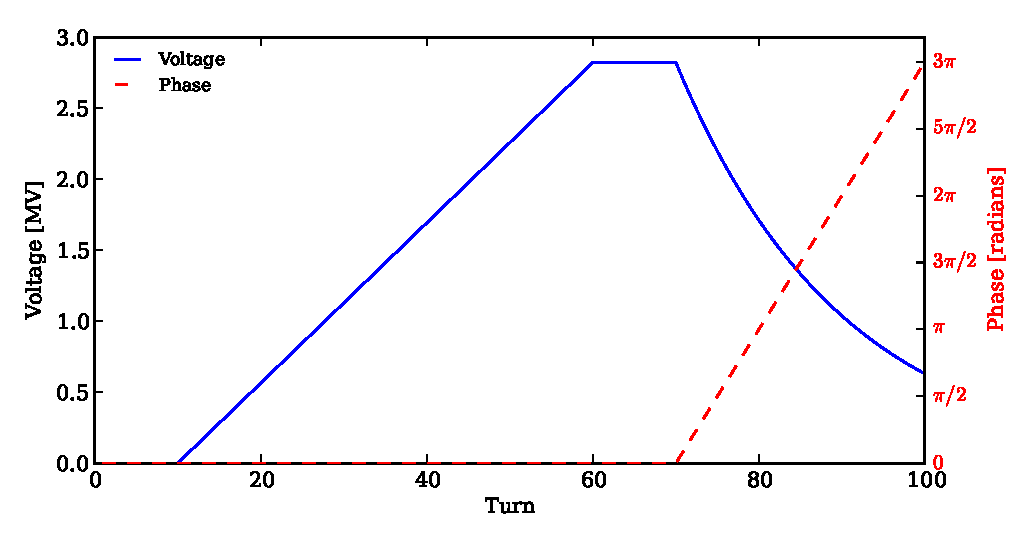
\includegraphics{figures/fail_voltagePhase2v2}
  \caption{Singals generate by \texttt{DYNK} example for ramp + exponential decay of crab voltage\index{crab cavity}\index{crab voltage}, and also linear drift of crab phase. Only the signals for CRAB\_IP1\_L1 are shown. The plot is made from the data in \texttt{dynksets.dat}.}
  \label{fig:DYNK_fail}
\end{figure}

This slightly more complicated example builds on the example given above.
It shows how to change two parameters (voltage and phase) of several objects.
It also demonstrates how functions can be chained together, making more complicated functions.
Some of the resulting functions are shown in Figure~\ref{fig:DYNK_fail}, and the \texttt{DYNK} block here looks like:
\begin{cverbatim}
DYNK
/DEBUG
FUN zero CONST 0.0
FUN CV_R1 GET CRAB_IP1_R1 voltage
FUN CV_R2 GET CRAB_IP1_R2 voltage
FUN CV_R3 GET CRAB_IP1_R3 voltage
FUN CV_R4 GET CRAB_IP1_R4 voltage
FUN CV_L  GET CRAB_IP1_L1 voltage
FUN ramp LIN 0.02 0
FUN ramp_R1 MUL CV_R1 ramp
FUN ramp_R2 MUL CV_R2 ramp
FUN ramp_R3 MUL CV_R3 ramp
FUN ramp_R4 MUL CV_R4 ramp
FUN ramp_L  MUL CV_L  ramp
SET CRAB_IP1_R1 voltage zero 1 10 0
SET CRAB_IP1_R2 voltage zero 1 10 0
SET CRAB_IP1_R3 voltage zero 1 10 0
SET CRAB_IP1_R4 voltage zero 1 10 0
SET CRAB_IP1_L1 voltage zero 1 9 0
SET CRAB_IP1_L2 voltage zero 1 9 0
SET CRAB_IP1_L3 voltage zero 1 9 0
SET CRAB_IP1_L4 voltage zero 1 9 0
/
SET CRAB_IP1_R1 voltage ramp_R1 11 61 -11
SET CRAB_IP1_R2 voltage ramp_R2 11 61 -11
SET CRAB_IP1_R3 voltage ramp_R3 11 61 -11
SET CRAB_IP1_R4 voltage ramp_R4 11 61 -11
SET CRAB_IP1_L1 voltage ramp_L 10 60 -10
SET CRAB_IP1_L2 voltage ramp_L 10 60 -10
SET CRAB_IP1_L3 voltage ramp_L 10 60 -10
SET CRAB_IP1_L4 voltage ramp_L 10 60 -10
/
/Voltage decay and detuning
FUN expCore LIN -0.05 0.0
FUN decay EXP expCore
FUN decayScaled MUL decay CV_L
SET CRAB_IP1_L1 voltage decayScaled 70 100 -70
SET CRAB_IP1_L2 voltage decayScaled 70 100 -70
SET CRAB_IP1_L3 voltage decayScaled 70 100 -70
SET CRAB_IP1_L4 voltage decayScaled 70 100 -70
FUN phasedrift LIN 0.3141592654 0.0
SET CRAB_IP1_L1 phase phasedrift 70 100 -70
SET CRAB_IP1_L2 phase phasedrift 70 100 -70
SET CRAB_IP1_L3 phase phasedrift 70 100 -70
SET CRAB_IP1_L4 phase phasedrift 70 100 -70
NEXT
\end{cverbatim}
The first functions defined here are the same as above, storing the default values (as defined in the single element list) for the relevant elements and also zero.
Then follows a normalized linear ramp function \texttt{ramp}, with gradient $0.02 = 1/50$.
This is then used by the ``specialized'' ramp functions \texttt{ramp\_R1$\cdots$R4}, which scales \texttt{ramp} so that the end point is the standard voltages for $t\in 0\ldots50$.

These functions are used to first set the crabs to $0.0$ for the first $9$ revolutions, and in the 10th revolution the ramp starts.
As the \texttt{ramp} function is defined starting at turn $0$, a shift $-10$ or $-11$ is applied to the ramps.
The ramp is switched off after turn 60/61, leaving the crabs to be operating at the last \texttt{SET} value.

Further, we want to demonstrate a failure in the crab voltage\index{crab voltage}.
This is done using an exponential decaying function $V(t) = V_0 \exp\left(-0.05 t\right)$, which is implemented as three chained functions:

\bigskip
\begin{tabular}{@{}lp{0.8\linewidth}}
    \textbf{expCore}     & $f(t) = -0.05 t + 0.0$ \\
    \textbf{decay}       & $g(t) = \exp(f(t)) = \exp(-0.05 t + 0.0)$ \\
    \textbf{decayScaled} & $h(t) = V_0 \cdot g(f(t)) = V_0 \cdot \exp(f(t)) = \exp(-0.05 t + 0.0)$
\end{tabular}

\bigskip
For the \texttt{SET}, the time $t$ is then shifted by $-70$ turns, so that the functions are evaluated starting at $t=0$.

\paragraph{Detuning a cavity (accelerating or crab)}~\\
\todo[inline]{Write}

\paragraph{Using the PIPE function}~\\
%Note: This example is referenced from the FUN table.

To use the \texttt{PIPE} functionality, add a \texttt{FUN} and \texttt{SET} to the \texttt{DYNK} block such as:
\begin{cverbatim}
FUN pipe1 PIPE /tmp/pip1 /tmp/pip2 myID1 4242
SET  ACFCA.AR1.B1 voltage pipe1 10 -1 -9
\end{cverbatim}
Then create the two pipes using the \texttt{mkfifo} UNIX command, e.g.\ \texttt{mkfifo~pip1} and \texttt{mkfifo~pip2} in the chosen directory.
When starting SixTrack, it will first open the input pipe (while reading the \texttt{DYNK} block), and wait for the external program to do the same.
This can be simulated by running \texttt{cat~>~pip1}; it is also possible to open the input pipe before starting SixTrack.
After opening the input pipe, SixTrack will open the output pipe, again this can be simulated by running \texttt{cat~pip2}, and again this pipe may be opened before starting SixTrack.
Note that when SixTrack ends, the output pipe will be closed, so the receiving \texttt{cat} process is terminated.

After opening the output pipe, SixTrack writes the line \texttt{DYNKPIPE~!******************!} to this file.
It then writes a line similar to \texttt{INIT~ID=myID1~for~FUN=pipe1} for each \texttt{FUN} using this output pipe.

During tracking, when one of the \texttt{PIPE} \texttt{FUN}s are called SixTrack writes a line similar to \texttt{GET ID=myID1 TURN=~1} to the output pipe.
Note that the turn number is the one passed to the \texttt{FUN} from \texttt{SET}, i.e. including any turn-shift.
It then waits for a single floating point number to be written (in ascii) to the input pipe, which is then read and returned from the \texttt{FUN}.

% ================================================================================================================================ %
\section{Beam--Beam Element} \label{BeamBeam}

The beam--beam kick, including a separation of the beams, is treated \`{a} la Basetti and Erskine~\cite{BasErs} and implemented as in MAD-X~\cite{MAD}.\index{beam--beam}\index{BEAM}
However, a much faster but nevertheless precise calculation using interpolation can be used~\cite{ERIC}.
Since SixTrack version 3, the beam--beam is also available in the 6D form \`{a} la Hirata~\cite{Hirata}.
Lastly, the linear coupling has been considered in 4 and 6 dimensional phase space~\cite{ripbeam}.

\bigskip
\begin{tabular}{@{}lp{0.8\linewidth}}
    \textbf{Keyword}    & \texttt{BEAM}\index{BEAM} \\
    \textbf{Data lines} & $>1$ \\
    \textbf{Format}     & Two different input formats are available, ``traditional'' and ``EXPERT''. If ``EXPERT'' mode is wanted, this is triggered by adding the flag \texttt{EXPERT}\index{BEAM EXPERT} on the first line of the block.
\end{tabular}

\paragraph{Traditional format}~\\

\bigskip
\begin{tabular}{@{}lp{0.8\linewidth}}
    First line:    & \texttt{partnum emitnx emitny sigz sige ibeco ibtyp lhc ibbc} \\
    Further lines: & \texttt{name ibsix xang xplane xstr}
\end{tabular}

\bigskip
\begin{longtabu}{@{}llp{0.65\linewidth}}
    \texttt{partnum}       & float   & Number of particles in bunch \\
    \texttt{emitnx,emitny} & floats  & Horizontal and vertical normalised emittance\index{normalised emittance} respectively [$\mu \mbox{m}\cdot\mbox{rad}$] \\
    \texttt{sigz,sige}     & floats  & r.m.s. bunch length [m] and r.m.s. energy spread \\
    \texttt{ibeco}         & integer & Switch (0 = off; 1 = on) to subtract the closed orbit introduced by the separation of the beams. It is recommended to always subtract it as it is not yet calculated in a selfconsistent manner. The \texttt{ibeco} switch also acts on the ``wire'' elements \ref{sec:WIRE} in the same way as on the beam-beam elements. It subtracts the closed orbit introduced by the wire if \texttt{ibeco}=1 and applies it if \texttt{ibeco}=0. \\
    \texttt{ibtyp}         & integer & Switch (0 = off; 1 = on) to use the fast beam--beam algorithms developed in collaboration with G.A.~Erskine and E.~McIntosh.  The linear optics are calculated with ``exact'' beam--beam kicks. \\
    \texttt{lhc}           & integer & For the LHC with its anti-symmetric IR the separation of the beams in one plane can be calculated by the $\beta$-function of the other plane. For flat beams (not anti-symmetric optics) the separation can be loaded from the \texttt{fort.2} file. (0 = off; 1 = anti-symmetric; 2 = load from file). \\
    \texttt{ibbc}          & integer & Linear coupling considered in 4D and 6D (0 = off; 1 = on). \\
    \texttt{name}          &           & Name of 6D beam--beam element. Beam--beam elements that do not appear will be treated as 4D kicks. \\
    \texttt{ibsix}         & integer & Number of slices of the 6D beam--beam element. If \texttt{ibsix} is set to 0 this element is treated as a 4D element. \\
    \texttt{xang}          & float   & Half crossing angle\index{half crossing angle} (angle the between the trajectories of the two beams) at this particular element [rad]. \\
    \texttt{xplane}        & float   & Crossing plane angle [rad]. \\
    \texttt{xstr}          & float   & Angle of the position of the slices in the boosted frame [rad] (i.e. $X = Z \sin(\mathit{xstr}) \cos(\mathit{xplane})$, $Y =Z \sin(\mathit{xstr}) \cos(\mathit{xplane})$ ).  In absence of crabbing user should make sure \texttt{xstr=xang}; in case the \texttt{xstr} flag is not set then \texttt{xstr=xang} is assumed and a warning is printed (since version 4.5.45).
\end{longtabu}

\paragraph{EXPERT format}~\\

\bigskip
\begin{longtabu}{@{}lp{0.8\linewidth}}
    First line:   & \texttt{EXPERT}\index{BEAM EXPERT} \\
    Second line:  & \texttt{partnum emitnx emitny sigz sige ibeco ibtyp lhc ibbc} \\
    Further lines & 4D BB lens (1 line per element): \\
                  & ~~~~\texttt{name ibsix $\Sigma_{x,x}$ $\Sigma_{y,y}$ h-sep v-sep strength-ratio $\Sigma_{x,y}$} \\
                  & 6D BB lens (3 lines per element): \\
                  & ~~~~\texttt{name ibsix xang xplane h-sep v-sep} \\
                  & ~~~~\texttt{$\Sigma_{x,x}$ $\Sigma_{x,xp}$ $\Sigma_{xp,xp}$ $\Sigma_{y,y}$ $\Sigma_{y,yp}$} \\
                  & ~~~~\texttt{$\Sigma_{yp,yp}$ $\Sigma_{x,y}$ $\Sigma_{x,py}$ $\Sigma_{xp,y}$ $\Sigma_{xp,yp}$ strength-ratio}
\end{longtabu}

\bigskip
Some parameters are new or defined in a different way:

\bigskip
\begin{longtabu}{@{}llp{0.65\linewidth}}
    \texttt{lhc}   & integer & This parameter is kept for now only for RHIC studies when equal to 9. \\
    \texttt{name}  &         & Name of the beam--beam element. \\
    \texttt{ibsix} & integer & Number of slices of the 6D beam--beam element.\\
                   &         & If \texttt{ibsix} is set to 0, this element is treated as a 4D element.\\
                   &         & If \texttt{ibsix} is larger or equal 1, this element is treated as a 6D element. \\
    $\Sigma_{xx}$  & float   & Horizontal $\sigma$ for the strong beam\index{strong beam} $\rm{[mm^2]}$. \\
    $\Sigma_{yy}$  & float   & Vorizontal $\sigma$ for the strong beam $\rm{[mm^2]}$. \\
    $\Sigma_{xy}$  & float   & Coupled $\sigma$ for the strong beam $\rm{[mm^2]}$. Optional, used only if \texttt{ibbc=1}. \\
    \texttt{h-sep} & float   & Horizontal beam--beam separation\index{beam--beam separation} [mm] \\
    \texttt{v-sep} & float   & Vertical beam--beam separation [mm] \\
    \texttt{strength-ratio} & float & Strength ratio with respect to the nominal beam--beam kick strength\index{beam--beam kick}. This is useful to allow for splitting one beam--beam kick into several (longitudinally close by) kicks.\\
    $\Sigma_{i,j}$ & float   & Second order momenta matrix for the strong beam, in units of mm and mrad. For example $\Sigma_{xxp}$ in [mm\ mrad]
\end{longtabu}

\paragraph{Conversion from traditional to EXPERT format}~\\

An automatic converter from the ``traditional'' input block to the new ``expert'' format is built into SixTrack; every time a non-\texttt{EXPERT} input block is encountered, a conversion is printed to the standard output.
Therefore, all the user needs to do is to run SixTrack (number of turns does not matter) on an input file that should be converted, and follow the instructions which are printed at the beginning of the program output.

\paragraph{Remarks}~\\

These beam--beam elements have to appear in the single element list (\ref{NonEle}) (type 20).
If the ``traditional'' option is used in the \texttt{BEAM} block, the listing in the single element list must contain their horizontal and vertical beam--beam separations (see~\ref{BBS}).

\paragraph{Sign Convention}~\\

Some clarifications regarding the sign convention used for the separation and crossing angle variables.
%\todo[inline]{Check if applies to both ``traditional'' and ``EXPERT'' format.}

\paragraph{Separations:}~\\
\begin{enumerate}
    \item The separation is added to the transverse coordinates of each particles just before the beam-beam subroutines (see Fig.~\ref{fig:BB_sep}).
        \begin{eqnarray*}
            \tilde x_{i} = x_{i} + \mathrm{sep}_{x} - \mathrm{CO}_{x} \\
            \tilde y_{i} = y_{i} + \mathrm{sep}_{y} - \mathrm{CO}_{y}
        \end{eqnarray*}
    \item Lorentz boost\index{Lorentz boost} applied to the updated coordinates.
    \item The separation used for the actual beam-beam kick (sep$_{x,y,kick}$) is the difference between the centroid of the strong slice (X$^{\dag}$,Y$^{\dag}$) and the each particle (x$_i$,y$_i$).
    \item Antiboost to return to accelerator frame.
    \item The separation is removed and the closed orbit is added back. Tracking continues.
        \begin{eqnarray*}
            \tilde x_{i} = x_{i} - \mathrm{sep}_{x} + \mathrm{CO}_{x} \\
            \tilde y_{i} = y_{i} - \mathrm{sep}_{y} + \mathrm{CO}_{y}
        \end{eqnarray*}
\end{enumerate}
\begin{figure}[h]
    \begin{center}
    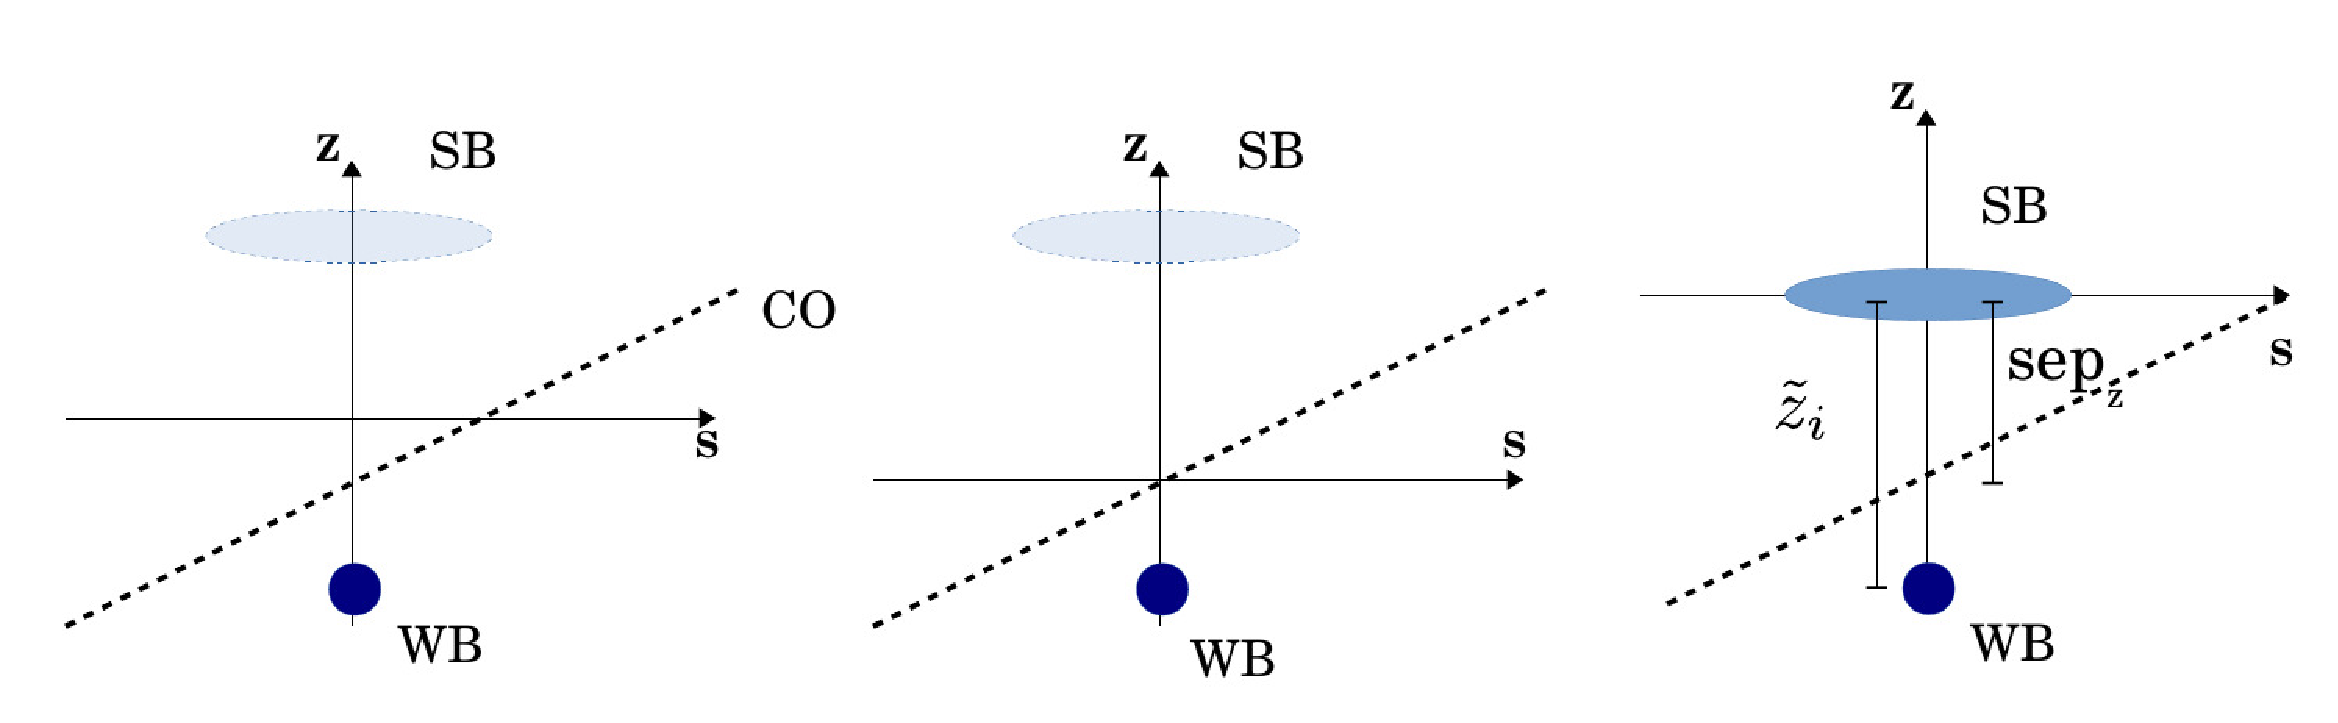
\includegraphics[width=0.8\textwidth]{figures/BB_sep}
    \caption{Coordinate manipulation taking into consideration the beam-beam lens separation as stated in point 1 of the separation sign convention.}
    \label{fig:BB_sep}
    \end{center}
\end{figure}

\paragraph{Crossing angles:}~\\
\begin{enumerate}
    \item The closed orbit\index{closed orbit} is removed just before the beam-beam subroutines.
        \begin{eqnarray*}
            \tilde x^{\prime}_{i} = x^{\prime}_{i} - \mathrm{CO}_{x^{\prime}} \\
            \tilde y^{\prime}_{i} = y^{\prime}_{i} - \mathrm{CO}_{y^{\prime}}
        \end{eqnarray*}
    \item Lorentz boost applied to the updated coordinates.
    \item Apply Synchro-Betatron Mapping\index{synchro-betatron mapping}.
    \item Antiboost to return to accelerator frame.
    \item The closed orbit\index{closed orbit} is added back. Tracking continues.
        \begin{eqnarray*}
            \tilde x^{\prime}_{i} = x^{\prime}_{i} + \mathrm{CO}_{x^{\prime}} \\
            \tilde y^{\prime}_{i} = y^{\prime}_{i} + \mathrm{CO}_{y^{\prime}}
        \end{eqnarray*}
\end{enumerate}
\begin{figure}[h]
    \begin{center}
    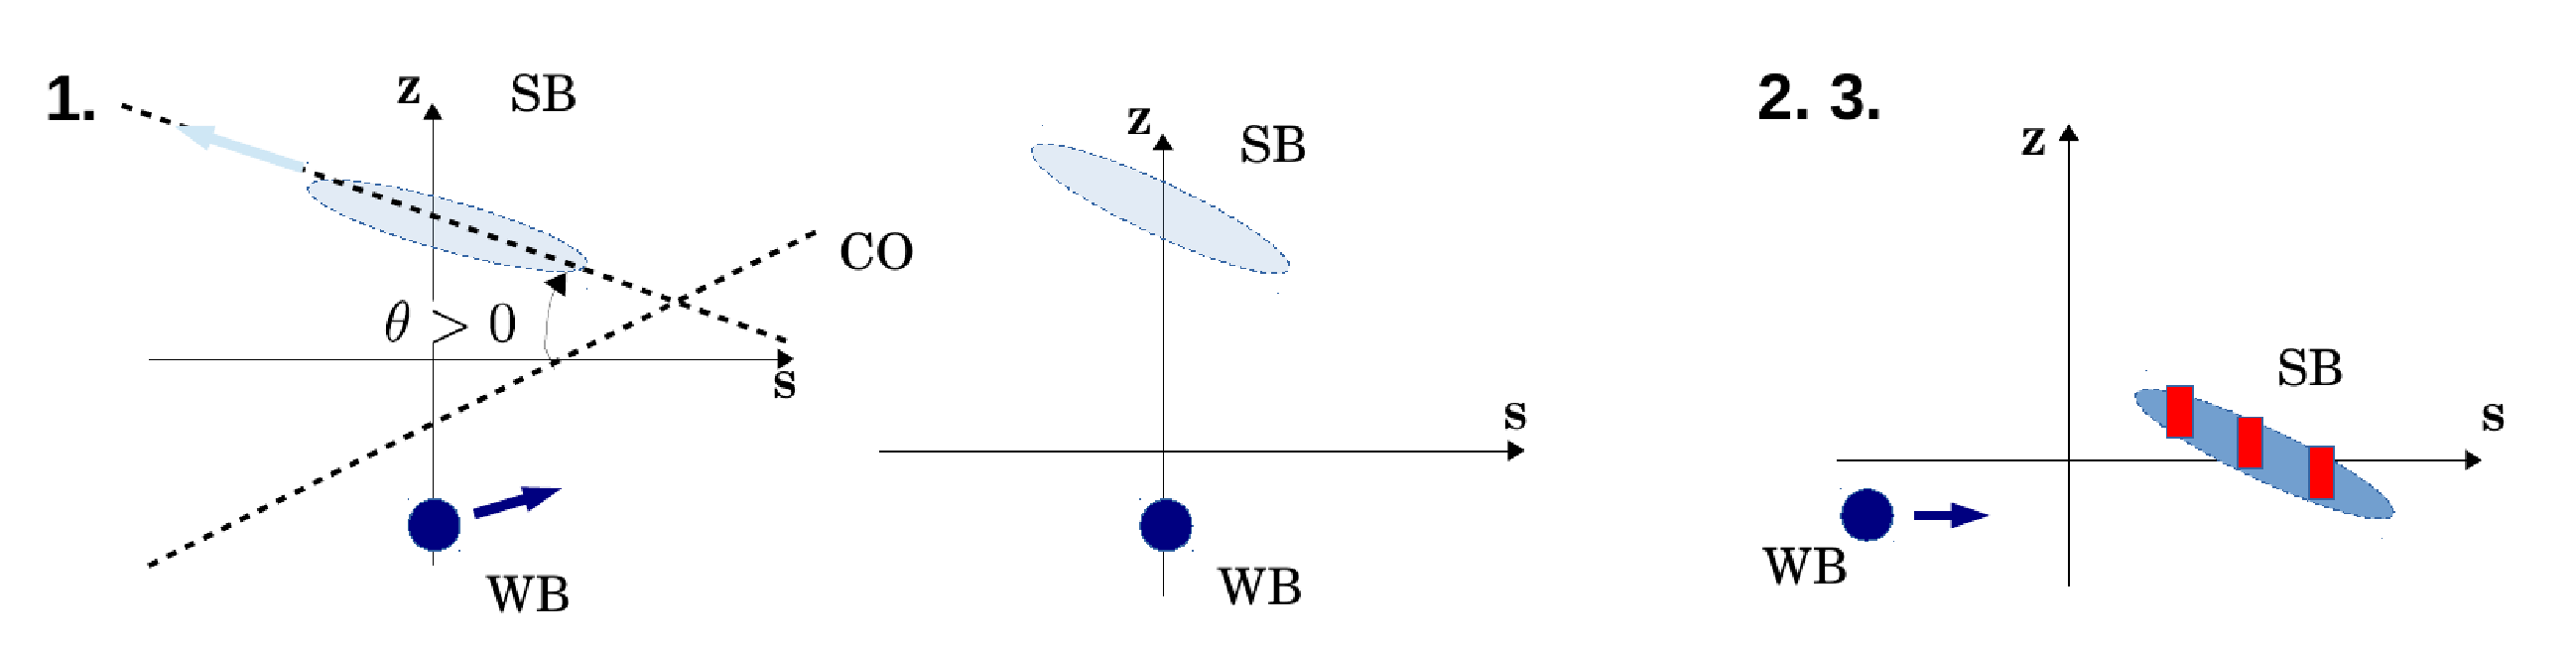
\includegraphics[width=0.8\textwidth]{figures/BB_xsing}
    \caption{Coordinate manipulation to move from the accelerator frame to a head-on collision frame (Figures left and center). A positive crossing angle is considered as shown in the left figure. Then Lorentz boost and Synchro-Betatron Mapping are applied (right).}
    \label{fig:BB_xsing}
    \end{center}
\end{figure}

% ================================================================================================================================ %
\section{Wire} \label{sec:WIRE}

The wire block serves for reading in the input parameters for the wire.\index{WIRE}
Each wire also needs to be added as single element in the list of single elements.

\bigskip
\begin{tabular}{@{}lp{0.8\linewidth}}
    \textbf{Keyword}    & \texttt{WIRE}\index{WIRE} \\
    \textbf{Data lines} & Variable \\
    \textbf{Format}     & \texttt{name flag\_co current int\_length phys\_length disp\_x disp\_y tilt\_x tilt\_y} \\
                        & A description of the input parameters for the wire is given in Table~\ref{tab:wire}.
\end{tabular}

\begin{center}
\begin{longtable}{|p{2.0cm} |p{1.4cm} |p{9.2cm}|}
    %Note: \\* (with the star) used to inhibit page breaks in the middle of groups of the same type
    \caption{Input parameters for the \texttt{WIRE} block.}
    \label{tab:wire} \\*
    \hline
    \rowcolor{blue!30}
    Arguments & Unit & Description \\*
    \hline
    \endfirsthead

    \hline
    \rowcolor{blue!30}
    Arguments & Unit & Description \\*
    %\hline
    \endhead

    \rowcolor{gray!15}
    \multicolumn{3}{|c|}{(The table continues on the next page)}\\*
    \hline
    \endfoot

    \hline
    \endlastfoot

    \hline

    \texttt{name} & - &
    Name of wire. Must be the same as in list of single elements\index{single elements}.\\*
    \hline

    \texttt{flag\_co} & - &
    flag to define the displacement of the wire in respect to the closed orbit\index{closed orbit} or x=y=0. For \texttt{flag\_co}=+1 \texttt{disp\_*} is the distance between x=y=0 and the wire. For \texttt{flag\_co}=-1 \texttt{disp\_*} is the distance between the closed orbit and the wire.\\*
    \hline

    \texttt{current} & A &
    wire current\index{wire current} \\*
    \hline

    \texttt{int\_length} & m &
    integrated length of the wire\\*
    \hline

    \texttt{phys\_length} & m &
    physical length of the wire\\*
    \hline

    \texttt{disp\_x} & mm &
    hor. displacement of the wire\\*
    \hline

    \texttt{disp\_y} & mm &
    vert. displacement of the wire\\*
    \hline

    \texttt{tilt\_x} & degrees &
    hor. tilt of the wire\index{wire tilt} $-90 < tilt\_x < 90$ (uses same defintion as DISP block) \\*
    \hline

    \texttt{tilt\_y} & degrees &
    vert. tilt of the wire $-90 < tilt\_y < 90$ (uses same defintion as DISP block) \\*
    \hline
\end{longtable}
\end{center}

\paragraph{Remarks}~\\

The user has to check that the wires defined in the WIRE block are also defined in the list of single elements and vice versa.
All parameters, except for the type (type 15), are ignored in the single element definition and the execution is aborted if the parameters are non-zero.
In addition to the parameters defined in the \texttt{WIRE} block, the \texttt{ibeco} parameter in the \texttt{BEAM} block (see Section~\ref{BeamBeam}) imposes the same behavior on the wire as for beam-beam.
Explicitly, the closed orbit introduced by the wire is subtracted if \texttt{ibeco}=1 and not subtracted if \texttt{ibeco}=0.

\paragraph{Example:}~\\

In the following we give some examples for wire definitions.
This example defines two wires \texttt{wire\_1} and \texttt{wire\_2}.

The input block in \texttt{fort.3} is given by:
\begin{cverbatim}
WIRE
wire_1   -1  +98.9   2.0  1.0   10.0   10.0     1.1     1.1
wire_2   -1  +98.9   2.0  1.0   10.0   10.0     0.0     0.0
NEXT
\end{cverbatim}
The single and structure element definition in \texttt{fort.2} is given by:
\begin{ctverbatim}
SINGLE ELEMENTS---------------------------------------------------------
...
wire_1   15 0.000000000e+00 0.000000000e+00  0.000000000e+00  0.000000000e+00  0.000000000e+00  0.000000000e+00
wire_2   15 0.000000000e+00 0.000000000e+00  0.000000000e+00  0.000000000e+00  0.000000000e+00  0.000000000e+00
...
STRUCTURE INPUT---------------------------------------------------------
...
BLOC56            wire_1              wire_2
...
\end{ctverbatim}
Note that all parameters except for the type have to be set to 0 in the single element definition.

% ================================================================================================================================ %
\section{``Phase Trombone'' Element} \label{Trombone}

The linear ``phase trombone'' allows for the introduction of an arbitrary transfer matrix.\index{phase trombone}\index{TROM}
It can be used to introduce a change in the transverse phases without spoiling the linear optics of the rest of the machine, i.e. the Twiss parameters are the same at entrance and exit of the element.
Note that it is up to the user to construct the matrix. The coordinates used as inputs are: $x$, $p_x$, $y$ ,$p_y$, $\sigma$, $p_{\sigma}$.

\bigskip
\begin{tabular}{@{}lp{0.8\linewidth}}
    \textbf{Keyword}    & \texttt{TROM}\index{TROM} \\
    \textbf{Data lines} & 1 line with name and then in blocks of 14 lines with 3 entries each. \\
    \textbf{Format}     & First line: \texttt{name} \\
                        & Second line:  $x$, $p_x$, $y$ \\
                        & Third line:  $p_y$, $\sigma$, $p_{\sigma}$ \\
                        & Fourth util $15^{th}$: \texttt{M($ 6 \times 6$)} matrix
\end{tabular}

\bigskip
\begin{tabular}{@{}llp{0.6\linewidth}}
    \texttt{name} & char & May contain up to 48 characters. \\
    \texttt{cx, cx', cy, cy', cz, cz'} & floats & 6D closed orbit\index{closed orbit} to be added to the coordinates. \\
    \texttt{M($ 6 \times 6$)} & floats & $ 6 \times 6$ matrix elements.
\end{tabular}

\paragraph{Remarks}~\\

The user has to make sure that the above stated conditions are fulfilled.
When using the $mad\_6t$~\cite{CONVERTOR} converter from MAD-X\index{MAD-X} to SixTrack, this is guaranteed to be the case.
Note also that the crossterms between the transverse plains are not considered for the time being.

% ================================================================================================================================ %
\section{Beam Distribution EXchange (BDEX)} \label{sec:BDEX}

The Beam Distribution EXchange allows an external program to read and modify the beam distribution in SixTrack.\index{BDEX}
This can be used for tracking part of the machine in an external program, for example for including physics processes that are normally not available in SixTrack.
Another possible use is for multi-bunch tracking, i.e.\ with an external program ``swapping'' the bunch at a some point in the ring.
This would be useful for studying (for example) beam loading, where the external program would read the position of a bunch in the cavity, use that to compute an update of the cavity voltage (which can be sent to SixTrack using DYNK FUN PIPE), swap the bunch with another one and track that to the cavity (still at ``physics turn'' 1, but ``SixTrack turn'' 2) etc.

Please note that \texttt{BDEX} is currently not supported in the checkpoint/restart\index{checkpoint/restart} version or in the collimation\index{collimation} version.
Including \texttt{BDEX} in one of these versions results in a run-time error.

\bigskip
\begin{tabular}{@{}lp{0.8\linewidth}}
    \textbf{Keyword}    & \texttt{BDEX}\index{BDEX} \\
    \textbf{Data lines} & Variable \\
    \textbf{Format}     & There are three types of statements possible in a \texttt{BDEX} block, listed below.
\end{tabular}

\bigskip

\paragraph{ELEM} \texttt{ELEM chanName elemName action}\\

This associates a given element with an already existing channel and an action.
The element must appear in the SINGLE ELEMENT\index{single elements} block, and be of type 0 (marker).
The action indicates what should be done with the particle distribution when it reaches this element.
Currently, the only allowed action is ``1'', which means ``particle exchange'', i.e.\ output the beam distribution and read back another one at the same point.

\paragraph{CHAN} \texttt{CHAN chanName chanType \ldots}\\

This creates a new channel through which the \texttt{BDEX} can communicate.
Currently, the only implemented \texttt{chanType} is \texttt{PIPE}, however \texttt{TCPIP} is also foreseen.

For the \texttt{PIPE} type, the statement including arguments is \texttt{CHAN PIPE inPipeName outPipeName format fileUnit}.
This uses a pair of UNIX FIFOs, through which SixTrack can communicate with an external program.
When the channel is used, it sends a message on the outpipe, then waits for a reply with the new distribution over the inPipe.
The \texttt{format} is an integer used to indicate the output/input format, and is currently unused.
The \texttt{fileUnit} is the Fortran unit number that should be used to open the inPipe.
The \texttt{outPipe} is opened on the next unit, so both units fileUnit and fileUnit+1 must be free.

\paragraph{DEBU}~\\

This statement switches on extra ``debugging'' output from \texttt{BDEX}\index{DEBUG}.
This can be useful if debugging the code or if debugging the input.

\subsection{Communication protocols}

The communication protocols used by the different channel types are listed below:

\paragraph{PIPE communication protocol}~\\

When a pair of pipes are first initialized, a header ``\texttt{BDEX-PIPE !******************!}'' is written to the output pipe.
Then, when the tracking reaches an element which is marked as active for this channel, it writes another header like ``\texttt{BDEX TURN= 1 BEZ=ip1 I= 1 NAPX= 64}'', where \texttt{TURN} is the number of the current SixTrack turn, \texttt{BEZ} the name of the SINGLE ELEMENT, \texttt{I} the index of the STRUCTURE ELEMENT, and \texttt{NAPX} the number of particles to be written out.
After this follows \texttt{NAPX} lines with the particle information (one per particle), each line of the format \texttt{xv(1,j) yv(1,j) xv(2,j) yv(2,j) sigmv(j) ejv(j) ejfv(j) rvv(j) dpsv(j) oidpsv(j) dpsv1(j),nlostp(j)} where all but the last floating point numbers, the last being an integer.
Finally, it writes ``\texttt{BDEX WAITING...}'' to the output pipe, and waits for data on the input pipe.

The first line expected on the input pipe should be an integer containing the number of particles to write back.
If this integer is -1, the current particle distribution is kept.
Otherwise, a number of lines of the same format as with the output is expected.
After reading in the expected number of particles, the string ``\texttt{BDEX TRACKING...}'' is written to the output pipe and tracking is resumed.

\paragraph{TCPIP communication protocol}~\\

TCPIP is not yet implemented, as it would require an external library.
The FLUKA version implements this, we should make sure that we are compatible with their requirements and ideally their protocol.

\paragraph{Example}~\\

\todo[inline]{Example BDEX block, example manual usage, example minimal Python program (location or listing).}

% ================================================================================================================================ %
\section{Electron lens} \label{sec:elen}

The electron lens module serves for reading in the input parameters for different types of electron lenses.\index{electron lens}\index{ELENS}
Each e--lens also needs to be added as single element in the list of single elements.
Currently the ideal electron lens is implemented, i.e.~with no errors in the e--beam distribution.

\bigskip
\begin{tabular}{@{}lp{0.8\linewidth}}
    \textbf{Keyword}    & \texttt{ELEN}\index{ELEN} \\
    \textbf{Data lines} & Variable \\
    \textbf{Format}     & \texttt{name type theta\_r2 r2 r1 offset\_x offset\_y (L I E\_k) } \\
                        & The last three parameters are optional, but if specified, all of them must be present; they allow to re-compute the angle at \texttt{r2}, taking into account also the beam energy.  \\
\end{tabular}

\begin{center}
\begin{longtable}{|p{2.0cm} | p{2.4cm} | p{1.0cm} | p{9.0cm}|}
    %Note: \\* (with the star) used to inhibit page breaks in the middle of groups of the same type
    \caption{Input parameters for \texttt{ELEN} block.}
    \label{tab:elen} \\*
    \hline
    \rowcolor{blue!30}
    Type Name & Arguments & Unit & Description \\*
    \hline
    \endfirsthead

    \hline
    \rowcolor{blue!30}
    Type Name & Arguments & Unit & Description \\*
    %\hline
    \endhead

    \rowcolor{gray!15}
    \multicolumn{4}{|c|}{(The table continues on the next page)}\\*
    \hline
    \endfoot

    \hline
    \endlastfoot

    \hline
    \rowcolor{blue!15}
    \multicolumn{4}{|l|}{Valid for all types} \\*

    & \texttt{name} & -- & Name of e--lens. Must be the same as in list of single elements\index{single elements}.\\*
    \hline

    & \texttt{type} & -- & Type of e--lens. Available type is only \texttt{UNIFORM}. \\* % and \texttt{GAUSSIAN}. \\*
    \hline

    & \texttt{theta\_r2} & mrad & Kick received at $r=r_2$ where $r_2$ is the outer radius of the e--lens.\\*
    \hline

    & \texttt{r2} & mm & Outer radius of the e--lens.\\*
    \hline

    & \texttt{r1} & mm & Inner radius of the e--lens. \\* % Can be 0 but not negative.\\*
    \hline

    & \texttt{offset\_x} & mm & Horizontal offset of the e--lens.\\*
    \hline

    & \texttt{offset\_y} & mm & Vertical offset of the e--lens.\\*
    \hline
    
    \hline
    \rowcolor{blue!15}
    \multicolumn{4}{|l|}{Optional arguments (all types)} \\*

    & \texttt{L} & m & Length of the e--lens. Must be positive. \\*
    \hline
    
    & \texttt{I} & A & Electron current of the e--lens. Must be non--zero. If negative, the electron beam is considered travelling in the direction opposite to the one of the main beam. \\*
    \hline
    
    & \texttt{E\_k} & keV & kinetic energy of electrons in the e--lens. Must be positive.\\*
    \hline

%     \rowcolor{blue!15}
%     \multicolumn{4}{|l|}{Type specific parameters} \\*
%     \texttt{GAUSSIAN} & \texttt{$\sigma$} & mm & Sigma of the e--beam.\\*
\end{longtable}
\end{center}

\noindent Currently, only one type of electron beam profiles is supported:

\bigskip
\begin{tabular}{@{}lp{0.8\linewidth}}
    \texttt{UNIFORM}  & e--beam with constant density of electrons. \\
%    \texttt{GAUSSIAN} & e--beam with a radial Gaussian profile. \\
\end{tabular}

\bigskip
\noindent The spacial charge density of all profiles is defined between \texttt{r1} and \texttt{r2}:
\begin{equation}
  \rho(r)=\left\{
    \begin{array}{ll}
        0 & \mbox{if $r \le r_1$} \\
        f(r) & \mbox{if $r_1 < r < r_2$} \\
        0 & \mbox{if $r_2 \le r$} \\
    \end{array}
    \right. \\
\end{equation}
%Moreover, if $r_1=0$, then the lens is full; otherwise, it is hollow.
For the time being, $r_1$ cannot be $0$; hence, the electron lens cann only be hollow.

\paragraph{Remarks}~\\

The user has to check that the e--lens defined in the \texttt{ELEN} block is also defined in the list of single elements and vice versa.
All parameters except for the type (type \texttt{29}) are ignored in the single element definition.
The implementation of the \texttt{UNIFORM} type (ideal e--lenses) has no explicit energy--dependency, except for the user defined parameter \texttt{theta\_r2} (see \cite{sixphys}). If \texttt{L}, \texttt{E\_k} and \texttt{I} are provided by the user, \texttt{theta\_r2} is re-calculated, taking into account the beam energy.

\paragraph{Examples}~\\

In the following we give some examples of e--lens definitions.
The example defines two electron lenses \texttt{hel1} and \texttt{hel2} with uniform electron density for cleaning purposes.
While the former has an explicit definition of the kick at \texttt{r2}, the latter triggers the re-computation of the angle, given the length of the electron lens of 4~m, the electron current of 1~A and the electron kinetik energy of 10~keV.
The input block in \texttt{fort.3} is then given by:
\begin{cverbatim}
ELEN
hel1 UNIFORM 4.920e-03 6.928 4.619 1.1547 2.3093
hel2 UNIFORM 4.920e-03 6.928 4.619 1.1547 2.3093 4 1 10
NEXT
\end{cverbatim}
The single and structure element definition in \texttt{fort.2} is given by:
\begin{ctverbatim}
SINGLE ELEMENTS---------------------------------------------------------
...
hel1            29  0.000000000e+00  0.000000000e+00  0.000000000e+00  0.000000000e+00  0.000000000e+00  0.000000000e+00
hel2            29  0.000000000e+00  0.000000000e+00  0.000000000e+00  0.000000000e+00  0.000000000e+00  0.000000000e+00
...
STRUCTURE INPUT---------------------------------------------------------
...
BLOC56            hel1              hel2
...
\end{ctverbatim}

\bigskip
\noindent \textbf{Note:} All parameters except for the type are set to 0 in the single element definition.

% ================================================================================================================================ %
\section{Scattering} \label{sec:scatter}

\textcolor{notered}{\textbf{Note:} This module is experimental! Use at your own risk; both the input format and physics implementation may change.}\index{scatter}\index{elastic scattering}\index{SCAT}

\bigskip
The \texttt{SCATTER} module is a framework for scattering particles through Monte Carlo processes at various points in the machine.

\bigskip
\begin{tabular}{@{}lp{0.8\linewidth}}
    \textbf{Keyword}    & \texttt{SCAT(TER)}\index{SCAT} \\
    \textbf{Data lines} & Variable \\
    \textbf{Format}     & There are several different main statement classes possible in a \texttt{SCATTER} block, listed below.
\end{tabular}

\bigskip

\paragraph{DEBUG} \texttt{DEBUG}\\

This statement switches on extra ``debugging'' output from \texttt{SCATTER}.
This can be useful if debugging the code or if debugging the input.

\paragraph{ELEMent} \texttt{ELEM elemname profile scaling gen1 (gen2, (gen3))}\\

This statements associates a \texttt{PRO}file and between one and 3\footnote{Controlled by the parameter \texttt{scatter\_maxGenELEM}.} \texttt{GEN}erators with a SINGLE ELEMENT which must be of type 40, as described in Section~\ref{SCAT}.
The \texttt{scaling} argument, which is a floating point number, is used to scale the probability of an interaction.
This can be controlled through DYNK, for example in order to scale only at one specified turn.
The \texttt{PRO}file, \texttt{GEN}erator(s), and single elements are referenced through their names, and for the \texttt{GEN}erators and \texttt{PRO}file they must be defined above the \texttt{ELEM}ent in the \texttt{SCATTER} block.

\paragraph{PROfile} \texttt{PRO name type (arguments)} \\

This statement defines a profile, that is a density profile and general properties of the targets which with the tracked particles are colliding.
Several different types are available:

\bigskip
\noindent\texttt{PRO name FLAT density[targets/cm$^2$] mass[MeV/c$^2$] momentum[MeV/c]}\\

\bigskip
\noindent\texttt{PRO name GAUSS1 beamtot[particles] sigmaX[mm] sigmaY[mm] offsetX[mm] offsetY[mm]} \\

The \texttt{GAUSS1} profile type us given by
\begin{align}
    \rho(x,y) = \frac{N_{\mathrm{tot}}}{2\pi\sigma_x\sigma_y}
                \exp\left(-\frac{(x-\mu_x)^2}{2\sigma_x^2}\right)
                \exp\left(-\frac{(y-\mu_y)^2}{2\sigma_y^2}\right).
\end{align}

\paragraph{GENerator} \texttt{GEN name type (arguments)} \\

The generator block takes a name and a generator type input, followed by the parameters for the
generator type.

\bigskip
\noindent\texttt{GEN name PPBEAMELASTIC a b1 b2 phi tmin (crossSection)} \\

Takes five or six input arguments, and generates the probability distribution given by
\begin{align}
    g(t) = \frac{1}{a_1^2}\frac{d\sigma}{dt} = e^{-b_1 t}+ 2ae^{-(b_1+b_2)t/2}\cos{\phi} + a^2e^{-b_2 t},
\end{align}
where the first expression is a soft scatter data fit, the third expression a hard scatter fit, and the second expression is the interference. $a = a_2/a_1$ is the amplitudes of the expressions.\index{elastic scattering}
These are combined into the first four input arguments $a$, $b_1$, $b_2$, and $\phi$, as well as $t_{min}$ which provides a cut-off limit.
The optional sixth argument defines a fixed cross section for the scattering probability.

Input example with values for a fit to 13 TeV LHC.
\begin{cverbatim}
GEN  sc_thin     PPBEAMELASTIC 0.046 18.52 4.601 2.647 0.0 30e-27
\end{cverbatim}

\paragraph{SEED} \texttt{SEED seed1 seed2}\\

This sets the seed of the internal RNG used by the \texttt{SCATTER} block \cite{RANECU}.
Two integer seeds are required, for this block.
The \texttt{SEED} block is mandatory for the \texttt{SCATTER} block to work.
Note that when running several simulations, the seed settings must be varied between each run in order to get uncorrelated results.

% ================================================================================================================================ %
\section{Tracking Code for Collimation Studies} \label{sec:collimat}

Collimation\index{collimation} and beam cleaning studies are carried out with the well established SixTrack code, extended for tracking large numbers of halo particles, and to take into account halo interaction with arbitrarily placed collimators.
Particles are transported through the lattice element by element and their phase space coordinates are transformed according to the type of element. When a particle hits a collimator jaw, it is randomly scattered through matter.
The effect of collimator scattering is modeled using COLLTRACK/K2 \cite{collimat:trenkler,collimat:robert_demolaize} routines.

\bigskip
\noindent The main characteristics of the SixTrack used for collimations studies are:
\begin{itemize}
    \item Proton scattering in various collimator materials, including:
    \begin{itemize}
        \item Multiple Coulomb scattering,
        \item Ionization of the collimator material,
        \item Elastic proton-proton (pp) scattering, and inelastic diffractive pp scattering (single diffractive scattering),
        \item Inelastic proton-nucleon scattering,
        \item Elastic and inelastic proton-nucleus scattering,
        \item Rutherford scattering.
    \end{itemize}
    \item Various types of halo and possibility of including diffusion.
    \item Tracking of large particle ensembles (~106 protons) over hundreds of turns.
    \item Multiple imperfections on the beam and the  collimator properties (setting errors, tilts, orbit, beta beat, …)
\end{itemize}

\bigskip
\noindent Input parameters are divided in 3 files:
\begin{itemize}
    \item \texttt{fort.2} (generated by MAD-X), defining the lattice of the machine without magnetic field errors.
    \item Collimator database file, containing the details of collimators geometry, material, settings (opening)
    \item \texttt{fort.3} (modified from the one used for SixTrack without collimation), including tracking parameters (number of particles and turns), type of beam, type of halo.
\end{itemize}

\noindent MAD-X is used to generate the LHC lattice, the optics and eventual orbit and focusing errors.
BeamLossPattern: Implementation of the LHC aperture model with analysis of loss locations for all tracked protons.

SixTrack for collimation studies tracks particles populating an halo (with typically $\sigma \geq 6$) throughout the LHC lattice (as defined by the MAD-X output file \texttt{fc.2}).
The halo is represented in the phase diagram $Y$ (offset from beam orbit axes), $Y^\prime$ (angle with respect to the beam orbit axes) in Figure~\ref{Coll:Fig1}.
\begin{figure}[H]
\begin{center}
    \includegraphics[width=0.5\linewidth]{figures/coll_fig1}
    \caption{\label{Coll:Fig1} \textbf{Left:} Halo particles in the phase diagram. \textbf{Right:} Impact Parameter.}
\end{center}
\end{figure}

One defines the Impact Parameter $b$ (see Figure~\ref{Coll:Fig1}) as the transverse offset between the jaw surface and the impact point.
$b$ typically equals $1\mu m$ at the first impact.

\bigskip
\noindent These changes implied to modify/add some input files:
\begin{itemize}
    \item the generic SixTrack parameter file \texttt{fort.3} now has a new block for collimation parameters,
    \item a separate collimator database file is now mandatory if collimation studies are to be done.
\end{itemize}

This database including the name, length, orientation and material of every single collimator of the ring (1 file per Collimation System Phase though).
Apart from these two, the other required SixTrack files are produced via MAD-X and its conversion module.

\paragraph{Collimator Database}~\\

The collimator database is stored in files named \texttt{CollDB\_V6.500\_[type]\_st.[beam].data}, with \texttt{[type]} being either inj for injection case or low $b$ for collision case, and \texttt{[beam]} being $b1$ or $b2$.
These files contain mechanical and optical data related to the collimators planned for LHC. (Note that at present only Phase I collimators have a length different from zero)

A sample block of either one of these input files follows:

\begin{cverbatim}
TCP.D6L7.B1             <-- collimator name in capital letters
tcp.d6l7.b1             <-- collimator name in minimal letters
5.7                     <-- collimator nominal opening (in sigma units)
C                       <-- collimator material (C = graphite, CU = copper, W=tungsten)
  0.2000000000000000    <-- collimator length [m]
  1.5710000000000000    <-- collimator angle [rad]
  0.0000000000000000    <-- collimator offset [m]
 90.4467000000000070    <-- design Beta x [m]
156.4360000000000070    <-- design Beta y [m]
#                       <-- line jump to next block
\end{cverbatim}

The introduction of the optic parameter $\beta$ allows studies of error scenarios (orbit distortion, beta-beating\index{beta-beating}) and/or to see the effect of misaligned collimators.
This structure is then repeated within the file for each of the collimators to be included in the study.

\subsection{Collimation Input Block} \label{sec:coll:input}

The collimation module is controlled by the \texttt{COLL} block in \texttt{firt.3}.

\bigskip
\begin{tabular}{@{}lp{0.8\linewidth}}
    \textbf{Keyword}    & \texttt{COLL}\index{COLL} \\
    \textbf{Data lines} & 17\\
    \textbf{Format}     & See below.
\end{tabular}

\paragraph{Format Description:}~\\

\bigskip
\begin{center}
\begin{longtable}{| p{0.5cm} | p{2.4cm} | p{1.2cm} | >{\raggedright\arraybackslash}p{11.4cm}|}
    \caption{Collimation input format.}
    \label{tab:COLL_INP} \\*
    \hline
    \rowcolor{blue!30}
    Ln & Keyword & Type & Description \\*
    \hline
    \endfirsthead

    \hline
    \rowcolor{blue!30}
    Ln & Keyword & Type & Description \\*
    \hline
    \endhead

    \rowcolor{gray!15}
    \multicolumn{4}{|c|}{(The table continues on the next page)}\\*
    \hline
    \endfoot

    \hline
    \endlastfoot

    1   & \texttt{DO\_COLL}      & logical & Switches on/off the collimation studies. \\
    \hline

    2   & \texttt{NLOOP}         & integer & Number of samples. No longer in use. Fixed to 1. \\
        \cline{2-4}
        & \texttt{MYENOM}        & float   & Energy of the beam to be tracked. \\
    \hline

    3   & \texttt{DO\_THISDIS}   & integer & Selects the type of distribution of the particles to be tracked (see below). \\
        \cline{2-4}
        & \texttt{MYNEX}         & float   & $A_x$ normalized amplitude of particles (in sigma units) in the $x$ direction. \\
        \cline{2-4}
        & \texttt{MDEX}          & float   & $\mbox{d}A_x$ smear (in sigma units) of the beam halo around $A_x$ (in $x$ direction). \\
        \cline{2-4}
        & \texttt{MYNEY}         & float   & $A_y$ normalized amplitude of particles (in sigma units) in the $y$ direction. \\
        \cline{2-4}
        & \texttt{MDEY}          & float   & $\mbox{d}A_y$ smear (in sigma units) of the beam halo around $A_y$ (in $y$ direction). \\
        \cline{2-4}
        & \texttt{FILENAME\_DIS} & char    & Name of the distribution file to be read if \texttt{DO\_THISDIS = 4/6}. \\
        \cline{2-4}
        & \texttt{ENERROR}       & float   & Energy spread of the tracked beam. Read only if \texttt{DO\_THISDIS = 3}. \\
        \cline{2-4}
        & \texttt{BUNCHLENGTH}   & float   & Bunch length of the tracked beam in millimeters. Read only if \texttt{DO\_THISDIS = 3}. \\
    \hline

    4   & \texttt{DO\_NSIG}      & logical & If TRUE use collimators settings from \texttt{fort.3}. If FALSE from \texttt{CollDB\_V6.500\_[type]\_st.[beam].data}. \\
        \cline{2-4}
        & \texttt{NSIG\_TCP3}    & float   & Opening of the primary collimator\index{primary collimator} in IR3 in sigma units. \\
        \cline{2-4}
        & \texttt{NSIG\_TCSG3}   & float   & Opening of the secondary graphite collimator in IR3 in sigma units\index{secondary collimator}. \\
        \cline{2-4}
        & \texttt{NSIG\_TCSM3}   & float   & Opening of the secondary metallic collimator in IR3 in sigma units\index{secondary collimator}. \\
        \cline{2-4}
        & \texttt{NSIG\_TCLA3}   & float   & Opening of the active absorbers in IR3 in sigma units\index{absorbers}. \\
        \cline{2-4}
        & \texttt{NSIG\_TCP7}    & float   & Opening of the primary collimators\index{primary collimator} in IR7 in sigma units. \\
        \cline{2-4}
        & \texttt{NSIG\_TCSG7}   & float   & Opening of the secondary graphite collimator in IR7 in sigma units\index{secondary collimator}. \\
        \cline{2-4}
        & \texttt{NSIG\_TCSM7}   & float   & Opening of the secondary metallic collimator in IR7 in sigma units\index{secondary collimator}. \\
        \cline{2-4}
        & \texttt{NSIG\_TCLA7}   & float   & Opening of the active absorbers collimator\index{absorbers} in IR7 in sigma units. \\
        \cline{2-4}
        & \texttt{NSIG\_TCLP}    & float   & Opening of the physics debris collimator in sigma units. \\
        \cline{2-4}
        & \texttt{NSIG\_TCLI}    & float   & Opening of the absorbers for injection protection in sigma units\index{absorbers}. \\
        \cline{2-4}
        & \texttt{NSIG\_TCDQ}    & float   & Opening of the beam dump protection collimator in sigma units\footnote{One-sided collimators (only positive x)}. \\
        \cline{2-4}
        & \texttt{NSIG\_TCSTCDQ} & float   & Opening of secondary collimator dedicated to beam dump in sigma units\index{secondary collimator}. \\
        \cline{2-4}
        & \texttt{NSIG\_TDI}     & float   & Opening of the injection protection collimator in sigma units. \\
    \hline

    5   & \texttt{NSIG\_TCTH1}   & float   & Opening of the horizontal tertiary collimator in IR1 in sigma units\index{tertiary collimator}. \\
        \cline{2-4}
        & \texttt{NSIG\_TCTH2}   & float   & Opening of the horizontal tertiary collimator in IR2 in sigma units\index{tertiary collimator}. \\
        \cline{2-4}
        & \texttt{NSIG\_TCTH5}   & float   & Opening of the horizontal tertiary collimator in IR5 in sigma units\index{tertiary collimator}. \\
        \cline{2-4}
        & \texttt{NSIG\_TCTH8}   & float   & Opening of the horizontal tertiary collimator in IR8 in sigma units\index{tertiary collimator}. \\
        \cline{2-4}
        & \texttt{NSIG\_TCTV1}   & float   & Opening of the vertical tertiary collimator in IR1 in sigma units\index{tertiary collimator}. \\
        \cline{2-4}
        & \texttt{NSIG\_TCTV2}   & float   & Opening of the vertical tertiary collimator in IR2 in sigma units\index{tertiary collimator}. \\
        \cline{2-4}
        & \texttt{NSIG\_TCTV5}   & float   & Opening of the vertical tertiary collimator in IR5 in sigma units\index{tertiary collimator}. \\
        \cline{2-4}
        & \texttt{NSIG\_TCTV8}   & float   & Opening of the vertical tertiary collimator in IR8 in sigma units\index{tertiary collimator}. \\
        \cline{2-4}
        & \texttt{NSIG\_TCXRP}   & float   & Opening of the Roman Pots in sigma units\footnote{One-sided collimators (only positive x)}. \\
        \cline{2-4}
        & \texttt{NSIG\_TCRYO}   & float   & Opening of the collimators in the DS regions in sigma units. \\
    \hline

    6   & \texttt{N\_SLICES}     & float   & Surface model of the jaw: number of slices in which each jaw should be cut. \\
        \cline{2-4}
        & \texttt{SMIN\_SLICES}  & float   & Surface model of the jaw: s position for the start of the slicing. \\
        \cline{2-4}
        & \texttt{SMAX\_SLICES}  & float   & Surface model of the jaw: s position for the end of the slicing. \\
        \cline{2-4}
        & \texttt{RECENTER1}     & float   & Surface model of the jaw: moving the 1st jaw to the new smallest opening. \\
        \cline{2-4}
        & \texttt{RECENTER2}     & float   & Surface model of the jaw: moving the 2nd jaw to the new smallest opening. \\
    \hline

    7   & \texttt{FIT1\_1}       & float   & Surface model of the jaw: order 0 of the polynomial fit for the 1st jaw. \\
        \cline{2-4}
        & \texttt{FIT1\_2}       & float   & Surface model of the jaw: order 1 of the polynomial fit for the 1st jaw. \\
        \cline{2-4}
        & \texttt{FIT1\_3}       & float   & Surface model of the jaw: order 2 of the polynomial fit for the 1st jaw. \\
        \cline{2-4}
        & \texttt{FIT1\_4}       & float   & Surface model of the jaw: order 3 of the polynomial fit for the 1st jaw. \\
        \cline{2-4}
        & \texttt{FIT1\_5}       & float   & Surface model of the jaw: order 4 of the polynomial fit for the 1st jaw. \\
        \cline{2-4}
        & \texttt{FIT1\_6}       & float   & Surface model of the jaw: order 5 of the polynomial fit for the 1st jaw. \\
        \cline{2-4}
        & \texttt{SSF1}          & float   & Surface model of the jaw: scaling factor of the polynomial fit for the 1st jaw. \\
    \hline

    8   & \texttt{FIT2\_1}       & float   & Surface model of the jaw: order 0 of the polynomial fit for the 2nd jaw. \\
        \cline{2-4}
        & \texttt{FIT2\_2}       & float   & Surface model of the jaw: order 1 of the polynomial fit for the 2nd jaw. \\
        \cline{2-4}
        & \texttt{FIT2\_3}       & float   & Surface model of the jaw: order 2 of the polynomial fit for the 2nd jaw. \\
        \cline{2-4}
        & \texttt{FIT2\_4}       & float   & Surface model of the jaw: order 3 of the polynomial fit for the 2nd jaw. \\
        \cline{2-4}
        & \texttt{FIT2\_5}       & float   & Surface model of the jaw: order 4 of the polynomial fit for the 2nd jaw. \\
        \cline{2-4}
        & \texttt{FIT2\_6}       & float   & Surface model of the jaw: order 5 of the polynomial fit for the 2nd jaw. \\
        \cline{2-4}
        & \texttt{SSF2}          & float   & Surface model of the jaw: scaling factor of the polynomial fit for the 2nd jaw. \\
    \hline

    9   & \texttt{EMITX0}        & float   & Geometric emittance in the horizontal plane. \\
        \cline{2-4}
        & \texttt{EMITY0}        & float   & Geometric emittance in the vertical plane. \\
    \hline

    10  & \texttt{DO\_SELECT}    & logical & Does dedicated study of selected collimator, see \texttt{NAME\_SEL}. \\
        \cline{2-4}
        & \texttt{DO\_NOMINAL}   & logical & Switches on/off the use of design $\beta$ values of collimators. \\
        \cline{2-4}
        & \texttt{RND\_SEED}     & integer & Seed studied. If set to 0, seed will be selected randomly for every run. \\
        \cline{2-4}
        & \texttt{DOWRITE\_DIST} & logical & Saves or not the initial distribution to be tracked. \\
        \cline{2-4}
        & \texttt{NAME\_SEL}     & char    & Name as in the \texttt{fort.2} file of the collimator one wants a dedicated study. \\
        \cline{2-4}
        & \texttt{DO\_ONESIDE}   & logical & Switches on/off the collimator being one-sided. Only positive jaw. If the negative jaw is to be used, it is necessary to turn collimator by 180 degrees in the collimator database file \texttt{CollDB\_V6.500\_[type]\_st.[beam].data}. \\
        \cline{2-4}
        & \texttt{DOWRT\_IMPACT} & logical & Saves the impact parameters for each collimator. \\
        \cline{2-4}
        & \texttt{DOWRT\_SECOND} & logical & Writes a secondary halo file based on normalized amplitude. \\
        \cline{2-4}
        & \texttt{DOWRT\_AMPL}   & logical & Writes checking files for amplitude, closed orbit. \\
    \hline

    11  & \texttt{XBEAT}         & float   & Offset in $x$ for the computation of collimator in case of beta-beating\index{beta-beating}. \\
        \cline{2-4}
        & \texttt{XBEATPHASE}    & float   & Phase offset in $x$ for the computation of collimator in case of beta-beating\index{beta-beating}. \\
        \cline{2-4}
        & \texttt{YBEAT}         & float   & Offset in $y$ for the computation of collimator in case of beta-beating\index{beta-beating}. \\
        \cline{2-4}
        & \texttt{YBEATPHASE}    & float   & Phase offset in $y$ for the computation of collimator in case of beta-beating\index{beta-beating}. \\
    \hline

    12  & \texttt{RMSTILT\_PRIM} & float   & RMS value of tilt to apply to primary collimators\index{primary collimator}. \\
        \cline{2-4}
        & \texttt{RMSTILT\_SEC}  & float   & RMS value of tilt to apply to secondary collimators\index{secondary collimator}. \\
        \cline{2-4}
        & \texttt{SYSTILT\_PRIM} & float   & Systematic value of tilt to apply to primary collimators.\index{primary collimator} \\
        \cline{2-4}
        & \texttt{SYSTILT\_SEC}  & float   & Systematic value of tilt to apply to secondary collimators\index{secondary collimator}. \\
        \cline{2-4}
        & \texttt{RMSOFFS\_PRIM} & float   & RMS value of offset to apply to primary collimators\index{primary collimator}. \\
        \cline{2-4}
        & \texttt{RMSOFFS\_SEC}  & float   & RMS value of offset to apply to secondary collimators\index{secondary collimator}. \\
        \cline{2-4}
        & \texttt{SYSOFFS\_PRIM} & float   & Systematic value of offset to apply to primary collimators\index{primary collimator}. \\
        \cline{2-4}
        & \texttt{SYSOFFS\_SEC}  & float   & Systematic value of offset to apply to secondary collimators\index{secondary collimator}. \\
        \cline{2-4}
        & \texttt{OFFTILT\_SEED} & float   & Random number seed to be used for the simulation. \\
        \cline{2-4}
        & \texttt{RMSERROR\_GAP} & float   & RMS error of collimator gap. \\
        \cline{2-4}
        & \texttt{DO\_MINGAP}    & logical & If TRUE the particle distribution is generated at the collimator with the smallest gap (to be used with sheet/pencil beam). \\
    \hline

    13  & \texttt{RADIAL}        & logical & Switches on/off the radial distribution. \\
        \cline{2-4}
        & \texttt{NR}            & float   & Size of the beam to be tracked in number of radial sigmas. \\
        \cline{2-4}
        & \texttt{NDR}           & float   & Smear of the beam to be tracked in number of radial sigmas. \\
    \hline

    14  & \texttt{DRIFTSX}       & float   & Apply an emittance drift\index{emittance drift} in the $x$ direction. \\
        \cline{2-4}
        & \texttt{DRIFTSY}       & float   & Apply an emittance drift\index{emittance drift} in the $y$ direction. \\
        \cline{2-4}
        & \texttt{CUT\_INPUT}    & logical & Formerly used to select particles to be tracked (set FALSE). \\
        \cline{2-4}
        & \texttt{SYSTILT\_ANTI} & logical & Deduce \texttt{SYSTILT} to \texttt{RMSTILT} instead of adding. \\
    \hline

    15  & \texttt{IPENCIL}       & integer & Resets original distribution to pencil beam\index{pencil beam} distribution on selected collimator. \\
        \cline{2-4}
        & \texttt{PENC\_OFFSET}  & float   & Size in sigma units of the desired impact parameter. \\
        \cline{2-4}
        & \texttt{PENC\_RMSX}    & float   & See table below. \\
        \cline{2-4}
        & \texttt{PENC\_RMSY}    & float   & See table below. \\
        \cline{2-4}
        & \texttt{PENC\_DISTR}   & integer & See table below. \\
    \hline

    16  & \texttt{COLL\_DB}      & char    & Name of the collimator database. \\
        \cline{2-4}
        & \texttt{IBEAM}         & integer & Number of the beam tracked (1 or 2). \\
    \hline

    17  & \texttt{DOWRITETRACKS} & logical & Writes secondary/tertiary halo files. \\
        \cline{2-4}
        & \texttt{CERN}          & logical & Switches on/off to cut halo files in separate pieces, one per 64 particles. \\
        \cline{2-4}
        & \texttt{CASTORDIR}     & char    & Name of the run; MUST BE EXACTLY 16 characters. \\
        \cline{2-4}
        & \texttt{JOBNUMBER}     & integer & 5 digit number, name of the complement to the name of the run (gives seed). \\
        \cline{2-4}
        & \texttt{SIGSECUT2}     & float   & Cut in square sigmas $x$/$y$ for saving particles (e.g. 64 for a cut at 8 $\sigma_x$/$\sigma_y$). \\
        \cline{2-4}
        & \texttt{SIGSECUT3}     & float   & Cut in square sigmas radial for saving particles (e.g. 90.25 for a cut at 9.5 $\sigma_r$). \\
    \hline
\end{longtable}
\end{center}

\paragraph{Pencil Beam Description:}~\\
\index{pencil beam}
\begin{tabular}{@{}l|p{0.6\linewidth}}
    \texttt{PENCIL\_DISTR = 0} & \texttt{PENC\_OFFSET  = 0} \\
    Pencil Beam Distribution   & \texttt{PENC\_RMSX    = 0} \\
                               & \texttt{PENC\_RMSY    = 0} \\
    \hline
    \texttt{PENCIL\_DISTR = 0} & \texttt{PENC\_OFFSET  = }center of rectangle \\
    Rectangular Distribution   & \texttt{PENC\_RMSX    = }spread of impact parameter (uniform) \\
                               & \texttt{PENC\_RMSY    = }spread parallel to jaw surface \\
    \hline
    \texttt{PENCIL\_DISTR = 1} & \texttt{PENC\_OFFSET  = }mean of Gaussian distribution \\
    Gaussian Distribution      & \texttt{PENC\_RMSX    = }spread of impact parameter (Gaussian) \\
                               & \texttt{PENC\_RMSY    = }spread parallel to jaw surface (Gaussian) \\
    \hline
    \texttt{PENCIL\_DISTR = 2} & \texttt{PENC\_OFFSET  = }mean of Gaussian distribution \\
    Half Gaussian Distribution & \texttt{PENC\_RMSX    = }spread of impact parameter (uniform) \\
                               & \texttt{PENC\_RMSY    = }spread parallel to jaw surface (Gaussian) \\
\end{tabular}

\bigskip
\noindent\textbf{Note:} The distribution with \texttt{PENCIL\_DISTR = 2} is used when wanting to simulate the loss of a magnet.


\paragraph{The \texttt{DO\_THISDIS} Flag Description:}
\begin{enumerate}
\item Distribution in the plane for which the parameters are specified ONLY: flat distribution in the selected plane between $A_x \pm \delta A_x$ (horizontal) or $A_y \pm \delta A_y$ (vertical). The amplitude in the other plane is zero\index{beam distribution}.
\item Distribution in the plane for which the parameters are specified + a Gaussian distribution cut at 3 s in the other plane.
\item Distribution in the plane for which the parameters are specified + a Gaussian distribution cut at 3 s in the other plane + energy spread given by \texttt{ENERROR} (nominally 3.06E-04 at 450GeV and 1.129E-04 at 7TeV) and a longitudinal component given by BUNCHLENGTH (nominally 11.24cm at 450GeV and 7.55cm at 7TeV).
\item Reads an external file that contains the beam distribution to be tracked.
\item Radial transverse distribution of radius Ar. This corresponds to a flat distribution both in the horizontal and vertical planes between $A_x \pm \delta A_x$ and $A_y \pm \delta A_y$, with $A_x = A_y = A_r/\ddot{O}2$.
\item Reads a normalised distribution from an external file.
\end{enumerate}

\paragraph{Examples}~\\

The following is an example collimation input block

\begin{cverbatim}
COLLIMATION----------------------------------------------------------------
    .TRUE.
    50   7000000
    3  5 .958  .0015  0.  0.  "nothing"  1. 129E-4  75.5
    .TRUE.  15.  18.  18.  20.  6.  7.  7.  10.0 1 0.0  999.0  8.0   7.5   999.0
    8.3  8.3  8.3  8.3  8.3  8.3  8.3  8.3  5. 15.
    0 19789.0  20150.0  1  1
   -1.3899e-6  -9.345e-5  5.05324e-3  -1.6595e-2  2.15955e-2  -9.96261e-3  1.0
   -1.3899e-6  -9.345e-5  5.05324e-3  -1.6595e-2  2.15955e-2  -9.96261e-3  1.0
    0.503E-09  0.503E-09
   .FALSE. .FALSE. 0 .TRUE. TCP.C6L7.B1 .FALSE. .TRUE. .TRUE. .TRUE.
   0.  0.  0.  0.
   0   0   0   0   0   0   0   0   0   0   .FALSE.
   .FALSE.  6.003  0.0015
   0.  0.  .FALSE. .FALSE.
   0   0.0025  0.0   0.0   0
   "CollDB_V6.500_lowb_st.b1.data"  1
   .TRUE. .FALSE. WAbsVertLowbcoll  101  1  1.
NEXT-----------------------------------------------------------------------------
\end{cverbatim}

\cleardoublepage
\input{chExternal}
\cleardoublepage

\chapter{Organising Tasks} \label{OrgTask}

In this chapter, the input data blocks used to organise the input structure are described.

% ================================================================================================================================ %
\section{Random Fluctuation Starting Number} \label{FluNum}

If besides mean values for the multipole errors (Gaussian) random errors should be considered, this input data structure is used to set the start value for the random generator.\index{random fluctuations}\index{random numbers}

\bigskip
\begin{tabular}{@{}lp{0.8\linewidth}}
    \textbf{Keyword}    & \texttt{FLUC}\index{FLUC} \\
    \textbf{Data lines} & 1 \\
    \textbf{Format}     & \texttt{izu0 mmac mout mcut} \/(integers)
\end{tabular}

\paragraph{Format Description}~

\bigskip
\begin{longtabu}{@{}lp{0.8\linewidth}}
    \texttt{izu0} & Start value for the random number generator \\
    \texttt{mmac} & Support for multiple starting seeds has been removed. This value must be 1. \\
    \texttt{mout} & A binary switch for various purposes, so all options, as described below, can be combined. \\
                  & \texttt{mout} = 0 : multipole errors internally created \\
                  & \texttt{mout} = 1 : multipole errors read-in from external file \\
                  & External multipole errors are read-in from file 16 into the array of random values. To activate these values one has to set to a value of 1 the relevant r.m.s.-positions of the corresponding multipole blocks (\ref{MulCoe}). The systematic components are added as usual and multipoles not found in the \texttt{fort.16}\index{fort.16} are treated as for (\texttt{mout} = 0). An error is only detected if there are too few sets of multipoles in \texttt{fort.16}. \\
                  & \texttt{mout} = 2: the geometry and strength file is written to file \texttt{fort.4}\index{fort.4} in the same format as the input file \texttt{fort.2}\index{fort.2}; the multipole coefficients are written to file \texttt{fort.9}; name, misalignments and tilt is written to file \texttt{fort.27}\index{fort.27} and finally name, random single multipole  strength and both random transverse misalignments are written to file \texttt{fort.31}\index{fort.31}.\\
                  & \texttt{mout} = 4: Name, horizontal and vertical misalignment and also the element tilt are read-in from file \texttt{fort.8}\index{fort.8}.\\
                  & \texttt{mout} = 8: Name and 3 Random numbers for single kick strength and both random transverse misalignments and also the value of the tilt are read-in from file \texttt{fort.30}. \\
    \texttt{mcut} & The random distribution can be cut by \texttt{mcut} sigma of the distribution. No cuts are applied for \texttt{mcut = 0}.
\end{longtabu}

\paragraph{Remarks}

\begin{enumerate}
    \item The \texttt{RANECU} random generator\index{random numbers} \cite{RANECU} is used as it produces machine independent sequences of random numbers.
    \item If the starting point has to be changed or another non-linear element is to be inserted, this can be done without changing the once chosen random distribution of errors by using the \textit{Organisation of Random Numbers} input block.
    \item The description of an accelerator is fully contained in 4 files: \texttt{fort.2} (geometry), \texttt{fort.3} (tracking parameters and definition of multipole blocks), \texttt{fort.16} (multipole errors) and \texttt{fort.30} (random numbers of the single multipole kick, the horizontal and vertical misalignment and the value of the tilt). This block allows to write  out the files \texttt{fort.4}\index{fort.4}, \texttt{fort.9}\index{fort.9}, \texttt{fort.27}\index{fort.27}, \texttt{fort.31}\index{fort.31} which may serve as the input files \texttt{fort.2}\index{fort.2}, \texttt{fort.16}\index{fort.16}, \texttt{fort.8}\index{fort.8} and \texttt{fort.30}\index{fort.30} respectively. The file \texttt{fort.30} supersedes \texttt{fort.8}\index{fort.8} if both files are read in.
\end{enumerate}

% ================================================================================================================================ %
\section{Organisation of Random Numbers} \label{OrgRan}

Working on a lattice for an accelerator often requires to introduce new non-linear elements.\index{random numbers}\index{ORGA}
In those cases simply introducing this new element means that the previously chosen random distribution of the errors will be changed and with it often the linear parameters.
This input data block is mainly used to avoid this problem by reserving extra random numbers for the new elements.
It also allows to change the observation point without affecting the machine.
The random values of different nonlinear elements including blocks of multipoles can be set to be equal to allow to vary the number of nonlinear kicks in one magnet which clearly should have the same random distribution for each multipolar kick.
Finally, multipole sets with different name can be made equal with this input data block.

\bigskip
\begin{tabular}{@{}lp{0.8\linewidth}}
    \textbf{Keyword}    & \texttt{ORGA}\index{ORGA} \\
    \textbf{Data lines} & Variable \\
    \textbf{Format}     & \texttt{ele1 ele2 ele3} \\
                        & The data lines can be set in three different ways described below.
\end{tabular}

\bigskip
\begin{longtabu}{@{}lp{0.8\linewidth}}
    Method 1 & \texttt{Ele1} = ``name'' where name $\ne$ \texttt{MULT} \\
             & \texttt{Ele2} = ignored  \\
             & \texttt{Ele3} = ignored  \\
             & The nonlinear element\index{non-linear elements} or multipole set will have its own set of random numbers. \\
    Method 2 & \texttt{Ele1} = ``name1'' where name1 $\ne$ \texttt{MULT} \\
             & \texttt{Ele2} = ``name2'' \\
             & \texttt{Ele3} = ignored \\
             & The nonlinear element or multipole block \texttt{Ele1} has the same random number set as those of \texttt{Ele2}, if it follows \texttt{Ele2} as the first non-linear element in the structure list (~\ref{StrInp}). \\
    Method 3 & \texttt{Ele1} = \texttt{MULT} \\
             & \texttt{Ele2} = ``name2'' \\
             & \texttt{Ele3} = ``name3'' \\
             & The multipole set ``name3'' is set to the values of the set ``name2''. random errors are not influenced in this case.
\end{longtabu}

\paragraph{Remarks}~

\begin{enumerate}
    \item A simple change of the starting point, by placing a \texttt{GO} somewhere in structure, used to change the machine optics as the random numbers were shifted, too. Simply calling this block even without a data line, will always fix the sequence of random numbers to start at the first multipole in the structure.
    \item This input data block must follow the definition of the multipole block, otherwise multipoles cannot be set equal (option 3).
    \item Do not use the keyword \texttt{MULT}\index{MULT} in the single element list (\ref{SinEle}).
\end{enumerate}

% ================================================================================================================================ %
\section{Combination of Elements} \label{ComEle}

It is often necessary to use several families of magnetic elements with a certain ratio $R$ of magnetic strength to perform corrections like tune adjustment (\ref{TunVar}), chromaticity correction (\ref{ChrCor}) or resonance compensation (\ref{ResCom})\index{combination of elements}.\index{COMB}
The \textit{Combination of Elements} input block allows such a combination of elements.
The maximum number of elements is defined by the parameter \texttt{NCOM} (see Appendix~\ref{DSP}).

\bigskip
\begin{tabular}{@{}lp{0.8\linewidth}}
    \textbf{Keyword}    & \texttt{COMB}\index{COMB} \\
    \textbf{Data lines} & Variable \\
    \textbf{Format}     & \texttt{e0 R1 e1 \dots~Rn en}
\end{tabular}

\paragraph{Format Description}~

\bigskip
\begin{tabular}{@{}lp{0.8\linewidth}}
    \texttt{e0} & Reference element which appears in the input of the processing procedure \\
    \texttt{e1, \dots, en} & Elements to be combined with \texttt{e0} \\
    \texttt{Rj} & Ratio of the magnetic strength\index{magnet strength} of element \texttt{ej} to that of element \texttt{e0}
\end{tabular}


\cleardoublepage

\chapter{Processing} \label{Proc}

This chapter comprises all the input blocks that do some kind of pre- or post-processing.

% ================================================================================================================================ %
\section{Linear Optics Calculation} \label{LinOpt}

The linear optics calculation input block is used to make a print-out of all linear parameters (magnet lengths, $\beta$ and $\alpha$ functions, tunes, dispersion and closed orbit) in the horizontal and vertical planes at the end of each element or linear block.\index{linear optics}\index{LINE}
The number of elements or blocks can be chosen.

\bigskip
\begin{tabular}{@{}lp{0.8\linewidth}}
    \textbf{Keyword}    & \texttt{LINE}\index{LINE} \\
    \textbf{Data lines} & $\geq 1$ \\
    \textbf{Format}     & First line: \texttt{mode num\_blocks ilin ntco E\_I E\_II} \\
                        & Other lines: \texttt{name(1), \dots , name(nlin)}
\end{tabular}

\paragraph{Format Description}~

\bigskip
\begin{longtabu}{@{}llp{0.7\linewidth}}
    \texttt{mode}        & char    & \texttt{ELEMENT} for a printout after each single element (\ref{SinEle}). \\
                         &         & \texttt{BLOCK} for a printout after each structure block (\ref{BloDef}). \\
    \texttt{num\_blocks} & integer & The number of the blocks in the structure to which the linear parameter will be printed. If this number is set to zero or is larger than the number of blocks, the complete structure will be calculated. \\
    \texttt{ilin}        & integer & Logical switch to calculate the traditional linear optics calculation in 4D (\texttt{1 = ilin}) and with the DA approach 6D (\texttt{2 = ilin}). \\
    \texttt{ntco}        & integer & A switch to write out linear coupling parameters. \\
                         &         &  \texttt{ntco = 0}: no write-out. \\
                         &         &  \texttt{ntco $\neq$ 0}: write-out of all linear coupled (4D) parameters including the coupling angle. These parameters (name, longitudinal position, the phase advances at that location, 4   $\beta$-, $\alpha$- and $\gamma$-functions, 4 angles for coordinates and momenta respectively, plus the coupling angle [rad]) are written in ascii format on file \texttt{fort.11}. This write-out happens every \texttt{ntco} turns. \\
    \texttt{E\_I, E\_II} & floats  & The two eigen-emittances to be chosen to determine the coupling angle. They are typically set to be equal. \\
    \texttt{names}       & char    & For \texttt{nlin $\leq$ nele} element and block names the linear parameters are printed whenever they appear in the accelerator structure.
\end{longtabu}

\paragraph{Remarks}
\begin{itemize}
    \item To make this block work the Tracking Parameter block (\ref{TraPar}) has to used as well.
    \item When the \texttt{ELEMENT 0} option is used, a file \texttt{fort.34} is written with the longitudinal position, name, element type, multipole strength, $\beta$ functions and phase advances in the horizontal and vertical phase space respectively. This file is used as input for the \texttt{SODD} program~\cite{SODD} to calculate de-tuning and distortion terms in first and second order. A full program suite can be found at: /afs/cern.ch/group/si/slap/share/sodd
    \item If the \texttt{BLOCK} option has been used, the tunes may be wrong by a multiple of 1/2. This option is not active in the DA part (\texttt{2 = ilin}), which also ignores the (\texttt{NTCO}) option.
\end{itemize}

% ================================================================================================================================ %
\section{Tune Variation} \label{TunVar}

This input block initializes a tune adjustment with zero length quadrupoles.\index{tune variation}\index{TUNE}
This is normally done with two families of focusing and defocusing quadrupoles.
It may be necessary, however, to have a fixed phase advance between certain positions in the machine.
This can be done with this block by splitting the corresponding family into two sub-families which then are adjusted to give the desired phase advance.

\bigskip
\begin{tabular}{@{}lp{0.8\linewidth}}
    \textbf{Keyword}    & \texttt{TUNE}\index{TUNE} \\
    \textbf{Data lines} & 2 or 4 \\
    \textbf{Format}     & Line 1: \texttt{name1 Qx iqmod6} \\
                        & Line 2: \texttt{name2 Qy} \\
                        & Line 3 (optional): \texttt{name3 $\Delta Q$} \\
                        & Line 4 (optional): \texttt{name4 name5}
\end{tabular}

\paragraph{Format Description}~

\bigskip
\begin{longtabu}{@{}llp{0.65\linewidth}}
    \texttt{name1, name2} & char    & Names of focusing and defocusing quadrupole\index{quadrupole} families respectively (in the single element list (~\ref{LinEle}). \\
    \texttt{Qx, Qy}       & floats  & Horizontal and vertical tune \emph{including} the integer part. \\
    \texttt{iqmod6}       & integer & Switch to calculate the tunes in the traditional manner (\texttt{1 = iqmod6}) and with the DA approach including the beam-beam kick (\texttt{2 = iqmod6}). FixMe: This is out of date and does not match the source code. \\
    \texttt{name3}        & char    & Name of the second sub-family, where the first sub-family is one of the above (\texttt{name1} or \texttt{name2}). This second sub-family replaces the elements of the first sub-family between the positions marked by \texttt{name4} and \texttt{name5}. \\
    \texttt{$\Delta Q$}   & float   & Extra phase advance \emph{including} the integer part (horizontal or vertical depending on the first sub-family) between the positions in the machine marked by \texttt{name4} and \texttt{name5}.\\
    \texttt{name4, name5} & char    & Two markers in the machine for the phase advance $\Delta Q$ with the elements of the second sub-family between them
\end{longtabu}

\paragraph{Remarks}~\\

The integer has to be included as the full phase advance around the machine is calculated by the program.

% ================================================================================================================================ %
\section{Chromaticity Correction} \label{ChrCor}

The chromaticity can be adjusted to desired values with two sextupole family using this input block.\index{chromaticity correction}\index{CHRO}

\bigskip
\begin{tabular}{@{}lp{0.8\linewidth}}
    \textbf{Keyword}    & \texttt{CHRO}\index{CHRO} \\
    \textbf{Data lines} & 2 \\
    \textbf{Format}     & Line 1: \texttt{name1 $Q'_x$ ichrom} \\
                        & Line 2: \texttt{name2 $Q'_y$}
\end{tabular}

\paragraph{Format Description}~

\bigskip
\begin{longtabu}{@{}llp{0.65\linewidth}}
    \texttt{name1, name2} & char    & Names (in the single element list (\ref{NonEle}) of the two sextupole\index{sextupole} families. \\
    \texttt{$Q^\prime$}   & float   & Desired values of the chromaticity\index{chromaticity}: $Q^\prime=\frac{\delta Q}{\delta( \frac{\Delta p}{p_o})}$. \\
    \texttt{ichrom}       & integer & Logical switch to calculate the traditional chromaticity calculation (\texttt{1}) and with the DA approach including the beam-beam kick (\texttt{2}). Setting this flag to \texttt{3} switches on both. \\
\end{longtabu}

\paragraph{Remarks}~\\

To make the chromaticity correction work well a small momentum spread is required (\texttt{DE0} in table (\ref{T-IteErr})).
It sometimes is required to optimize this spread.

% ================================================================================================================================ %
\section{Orbit Correction} \label{OrbCorr}

Due to dipole errors\index{dipole errors} in a real accelerator, a closed orbit\index{closed orbit} different from the beam axis is unavoidable.\index{orbit correction}\index{ORBI}
Even after careful adjustment, one always will be left over with some random deviation of the closed orbit around the zero position.
A closed orbit is introduced by non-zero strengths of $b_{1}$ and $a_{1}$ components of the multipole block (\ref{MulCoe}), horizontal and vertical dipole kicks (\ref{NonEle}), or displacements of non-linear elements (\ref{DisEle}).
This input data block allows the correction of a such a random distributed closed orbit using he first two types in a ``most effective corrector strategy'' \cite{Auti}.
For that purpose, correctors have to be denoted by \texttt{HCOR} and \texttt{VCOR}, and monitors by \texttt{HMON} and \texttt{VMON} for the horizontal and vertical plane respectively.
After correction, the orbit is scaled to the desired r.m.s. values, unless they are zero.

The horizontal orbit displacement\index{orbit displacement}, measured at the horizontal monitors\index{monitors}, will be written to \texttt{fort.28} -- together with the monitor number, in \texttt{fort.29}. The same is done for the vertical closed orbit displacement.

\bigskip
\begin{tabular}{@{}lp{0.8\linewidth}}
    \textbf{Keyword}    & \texttt{ORBI} \\
    \textbf{Data lines} & $\geq 1$ \\
    \textbf{Format}     & First line: \texttt{sigmax sigmay ncorru ncorrep} \\
                        & Other lines: \texttt{HCOR namec}, \texttt{HMON namem}, \texttt{VCOR namec} or \texttt{VMON namem}.\\
\end{tabular}

\paragraph{Format Description}~

\bigskip
\begin{longtabu}{@{}lp{0.75\linewidth}}
    \texttt{sigmax, sigmay} & Desired r.m.s.-values of the randomly distributed closed orbit. \\
    \texttt{ncorru}         & Number of correctors to be used. \\
    \texttt{ncorrep}        & Number of corrections. \\
                            & If \texttt{ncorrep=0}, the correction is iterated until \texttt{ITCO} iterations or after the both desired r.m.s.-values have been reached (see table~\ref{T-IteErr}). \\
    \texttt{HCOR=namec}     & Horizontal correction element of name \texttt{namec}. \\
    \texttt{HMON=namem}     & Horizontal monitor for the closed orbit of name \texttt{namem}. \\
    \texttt{VCOR=namec}     & Vertical correction element of name \texttt{namec}. \\
    \texttt{VMON=namem}     & Vertical monitor for the closed orbit of name \texttt{namem}.
\end{longtabu}

\paragraph{Remarks}~

\begin{itemize}
    \item Elements can have only one extra functionality: either horizontal corrector, horizontal monitor, vertical corrector or   vertical monitor. If the number of monitors in a plane is smaller than the number of correctors it is likely to encounter numerical problems.
    \item The \texttt{HCOR}, \texttt{HMON}, \texttt{VCOR}, and \texttt{VMON} must be separated from the following name by at least one space.
\end{itemize}

% ================================================================================================================================ %
\section{Decoupling of Motion in the Transverse Planes} \label{LinDec}

Skew quadrupole\index{skew quadrupole} components in the lattice create a linear coupling between the transverse planes of motion.\index{decoupling of motion}\index{DECO}
A decoupling can be achieved with this block using four independent families of skew-quadrupoles, which cancel the off-diagonal parts of the transfer map\index{transfer map}.
As these skew quadrupoles also influence the tunes an adjustment of the tunes is performed at the same time.

\bigskip
\begin{tabular}{@{}lp{0.8\linewidth}}
    \textbf{Keyword}    & \texttt{DECO}\index{DECO} \\
    \textbf{Data lines} & 3 \\
    \textbf{Format}     & Line 1: \texttt{name1,name2,name3,name4} \\
                        & Line 2: \texttt{name5 Qx} \\
                        & Line 3: \texttt{name6 Qy}
\end{tabular}

\paragraph{Format Description}~

\bigskip
\begin{tabular}{@{}llp{0.70\linewidth}}
    \texttt{name1,2,3,4} & char   & Names of the four skew quadrupole\index{skew quadrupole} families. \\
    \texttt{name5,6}     & char   & Names of focusing and defocusing quadrupole families respectively (in the single element list (\ref{LinEle}). \\
    \texttt{Qx, Qy}      & floats & Horizontal and vertical tune \emph{including} the integer part.
\end{tabular}

\paragraph{Remarks}~\\

A decoupling can also be achieved by compensating skew-resonances (\ref{ResCom}).
The two approaches, however, are not always equivalent.
In the resonance approach the zeroth harmonic is compensated, whilst a decoupling also takes into account the higher order terms.

% ================================================================================================================================ %
\section{Sub-Resonance Calculation} \label{SubCal}

First order resonance widths of multipoles from second to ninth order are calculated following the approach of Guignard \cite{Gilbert78}.\index{sub-resonance}\index{SUBR}
This includes resonances, which are a multiple of two lower than the order of the multipole.
The first order detuning including feed-down from closed orbit\index{closed orbit} is calculated from all multipoles up to to tenth order.

\bigskip
\begin{tabular}{@{}lp{0.8\linewidth}}
    \textbf{Keyword}    & \texttt{SUBR}\index{SUBR} \\
    \textbf{Data lines} & 1 \\
    \textbf{Format}     & \texttt{n1 n2 Qx Qy Ax Ay Ip length}
\end{tabular}

\paragraph{Format Description}~

\bigskip
\begin{longtabu}{@{}llp{0.75\linewidth}}
    \texttt{n1, n2} & integers & Lowest and highest order of the resonance. \\
    \texttt{Qx, Qy} & floats   & Horizontal and vertical tune including the integer part. \\
    \texttt{Ax, Ay} & floats   & Horizontal and vertical amplitudes in mm. \\
    \texttt{Ip}     & integer  & Is a switch to change the nearest distance to the resonance \mbox{$e = nxQx + nyQy$.} In cases of structure resonances a change of $p$ by one unit may be useful. \\
                    &          & \texttt{ip = 0}: $e$ is unchanged. \\
                    &          & \texttt{ip = 1}: \mbox{$(e \pm 1) = nxQx + nyQy - (p \pm 1)$}. \\
    \texttt{length} & float    & Length of the accelerator in meters
\end{longtabu}

% ================================================================================================================================ %
\section{Search for Optimum Places to Compensate Resonances} \label{SeaPla}

To be able to compensate a specific resonance, one has to know how a correcting multipole affects the cosine and sine like terms of the resonance width at a given position in the ring.\index{search}\index{SEAR}
This input data block can be used to find best places for the compensation of up to three different resonances, by calculating the contribution to the resonance width for a variable number of positions.
For each position, the effect of a fixed and small change of magnetic strength on those resonance widths is tested.

\bigskip
\begin{tabular}{@{}lp{0.8\linewidth}}
    \textbf{Keyword}    & \texttt{SEAR}\index{SEAR} \\
    \textbf{Data lines} & $\geq 2$ \\
    \textbf{Format}     & Line 1: \texttt{Qx Qy Ax Ay length} \\
                        & Line 2: \texttt{npos n ny1 ny2 ny3 ip1 ip2 ip3} \\
                        & Other lines: \texttt{name1, \dots , namen}
\end{tabular}

\paragraph{Format Description}~

\bigskip
\begin{longtabu}{@{}llp{0.65\linewidth}}
    \texttt{Qx, Qy}      & floats   & Horizontal and vertical tune\index{tune} including the integer part. \\
    \texttt{Ax, Ay}      & floats   & Horizontal and vertical amplitudes in mm. \\
    \texttt{length}      & float    & Length of the accelerator in m. \\
    \texttt{npos}        & integer  & Number of positions to be checked. \\
    \texttt{n}           & integer  & Order of the resonance. \\
    \texttt{ny1,ny2,ny3} & integers & Define three resonances of order $n$ via: \\
                         &          & \mbox{$nx Qx + ny Qy = p$} with \mbox{$\vert nx \vert + \vert ny \vert = n$}. \\
    \texttt{ip1,ip2,ip3} & integers & The distance to a resonance is changed by an integer $ip$ for each of the three resonances: \\
                         &          & \mbox{$e = nx Qx + ny Qy - (p + ip) $.} \\
    \texttt{namei}       & char     & The i-th name of a multipole of order $n$, which has to appear in the single element list (\ref{NonEle}).
\end{longtabu}

% ================================================================================================================================ %
\section{Resonance Compensation} \label{ResCom}

The input block allows the compensation of up to three different resonances of order $n$ simultaneously.\index{resonance compensation}\index{RESO}
The chromaticity\index{chromaticity} and the tunes can be adjusted.
For mostly academic interest, there is also the possibility to consider sub-resonances\index{sub-resounance}, which come from multipoles, which are a multiple of 2 larger than the resonance order $n$.
However, it must be stated that the sub-resonances depend differently on the amplitude compared to resonances where the order of the resonances is the same as that of the multipoles.

\bigskip
\begin{tabular}{@{}lp{0.8\linewidth}}
    \textbf{Keyword}    & \texttt{RESO}\index{RESO} \\
    \textbf{Data lines} & 6 \\
    \textbf{Format}     & Line 1: \texttt{nr n ny1 ny2 ny3 ip1 ip2 ip3} \\
                        & Line 2: \texttt{nrs ns1 ns2 ns3} \\
                        & Line 3: \texttt{length Qx Qy Ax Ay} \\
                        & Line 4: \texttt{name1, \dots, name6} \\
                        & Line 5: \texttt{nch name7 name8} \\
                        & Line 6: \texttt{nq name9 name10 Qx0 Qy0}
\end{tabular}

\paragraph{Format Description}~

\bigskip
\begin{longtabu}{@{}llp{0.65\linewidth}}
    \texttt{nr}          & integer  & Number of resonances (0 to 3). \\
    \texttt{n}           & integer  & Order of the resonance, which is limited to \texttt{nrco= 5} (see list of parameters in Appendix~\ref{DSP}). \mbox{normal: $3 \le n \le nrco$; skew: $2 \le n \le nrco$}. \\
    \texttt{ny1,ny2,ny3} & integers & Define three resonances of order $n$ via: \mbox{$nx Qx + ny Qy = p$} with \mbox{$\vert nx \vert + \vert ny \vert = n$}. \\
    \texttt{ip1,ip2,ip3} & integers & The distance to the resonance $e$ can be changed by an integer value: \mbox{$e = nx Qx + ny Qy - (p+ip)$.} \\
    \texttt{nrs}         & integer  & Number of sub-resonances (0 to 3). \\
    \texttt{ns1,ns2,ns3} & integers & Order of the multipole with \mbox{$ns \le 9$} and \mbox{$(ns-n)/2 \in {\mathbf N}$}. \\
    \texttt{length}      & float    & Length of the machine in meters. \\
    \texttt{Qx, Qy}      & floats   & Horizontal and vertical tune including the integer part. \\
    \texttt{Ax, Ay}      & floats   & Horizontal and vertical amplitudes in mm. \\
    \texttt{name1-6}     & char     & Names (\ref{NonEle}) of the correction multipoles for the first, second and third resonance. \\
    \texttt{nch}         & integer  & Switch for the chromaticity correction (0 = off, 1 = on). \\
    \texttt{name7,8}     & char     & Names (\ref{NonEle}) of the families of sextupoles to correct the chromaticity. \\
    \texttt{nq}          & integer  & Switch for the tune adjustment (0 = off, 1 = on). \\
    \texttt{name9,10}    & char     & Names (\ref{LinEle}) of the families of quadrupoles to adjust the tune. \\
    \texttt{Qx0, Qy0}    & floats   & Desired tune values including the integer part.
\end{longtabu}

% ================================================================================================================================ %
\section{Differential Algebra} \label{DifAlg}

This input block initiates the calculation of a one turn map using the LBL Differential Algebra package~\cite{DALIE}.\index{differential algebra}\index{SixDA}
The use of this block inhibits post-processing.
The same differential algebra tools allow a subsequent normal form analysis (see \cite{Forest89}).
A four-dimensional version integrated in SixTrack is available as described in sections~\ref{Normal} and~\ref{Corrections}.

\bigskip
\begin{tabular}{@{}lp{0.8\linewidth}}
    \textbf{Keyword}    & \texttt{DIFF} \\
    \textbf{Data lines} & 1 or 2 \\
    \textbf{Format}     & Line 1: \texttt{nord nvar preda nsix ncor} \\
                        & Line 2: \texttt{name(1),\ldots,name(ncor)}
\end{tabular}

\paragraph{Format Description}~

\bigskip
\begin{longtabu}{@{}llp{0.7\linewidth}}
    \texttt{nord}    & integer & Order of the map. \\
    \texttt{nvar}    & integer & Number of the variables (2 to 6).\\
                     &         & \texttt{nvar = 2,4,6}: two- and four-dimensional transverse motion and full six-dimensional phase space respectively. \\
                     &         & \texttt{nvar = 5}: four-dimensional transverse motion plus the relative momentum deviation \mbox{$\frac{\Delta p}{p_o}$} as a parameter. \\
    \texttt{preda}   & float   & Precision needed by the DA package, usually set to \mbox{\texttt{preda= 1e-38}}. \\
    \texttt{nsix}    & integer & Switch to calculate a $5 \times 6$ instead of a $6 \times 6$ map. This saves computational time and memory space, as the machine can be treated up to the cavity as five-dimensional (constant momentum ). \\
                     &         & \texttt{nsix = 0}: $6 \times 6$ map. \\
                     &         & \texttt{nsix = 1}: $5 \times 6$ map. \\
                     &         & (\texttt{\em nvar} must be set to 6; 6D closed orbit must not be calculated, i.e. \mbox{\texttt{iclo6 = 0}}~(\ref{IniCoo}) and the map calculation is stopped once a cavity has been reached and being    evaluated.) \\
    \texttt{ncor}    & integer & Number of zero-length elements to be additional parameters besides the transverse and/or longitudinal coordinates (i.e.~two-, four-, five- or six-dimensional phase space). \\
    \texttt{name(i)} & char    & \texttt{Ncor} names (\ref{NonEle}) of zero-length elements (e.g dipole kicks, quadrupole kicks,   sextupoles kicks etc.)
\end{longtabu}

\paragraph{Remarks}~
\begin{itemize}
    \item For \texttt{nsix = 1}, the map can only be calculated till a cavity is reached.
    \item If the 6D closed orbit is calculated, the $5 \times 6$ map cannot be done. \texttt{nsix} is therefore forced to 0.
    \item If \texttt{nvar} is set to 5, the momentum dependence is determined without the need for including a fake cavity. With other words: the linear blocks are automatically broken up into single linear elements so that the momentum dependence can be calculated.
    \item If a DA map is needed at some longitudinal location, one just has to introduce an element denoted \texttt{DAMAP} at that place in the structure, \texttt{DAMAP} has also to appear as a marker (zero length, element type = 0) in the single element list (\ref{NonEle}). This extra map is written to file \texttt{fort.17}.
\end{itemize}

% ================================================================================================================================ %
\section{Normal Forms} \label{Normal}

All the parameters to compute the Normal Form of a truncated one turn map are given in the \textit{Normal Form} input block.\index{normal forms}\index{NORM}
Details on these procedures including the next block~\ref{Corrections} can be found in reference \cite{Massimo}.

\bigskip
\begin{tabular}{@{}lp{0.8\linewidth}}
    \textbf{Keyword}    & \texttt{NORM}\index{NORM} \\
    \textbf{Data lines} & 1 \\
    \textbf{Format}     & \texttt{nord nvar}
\end{tabular}

\paragraph{Format Description}~

\bigskip
\begin{tabular}{@{}llp{0.7\linewidth}}
    \texttt{nord} & integer & Order of the Normal Form. \\
    \texttt{nvar} & integer & Number of variables.
\end{tabular}

\paragraph{Remarks}~
\begin{itemize}
    \item The \textit{Normal Form} input block has to be used in conjunction with the \textit{Differential Algebra} input block that computes the one turn map of the accelerator.\index{differential algebra}
    \item The value of the parameter \texttt{nord} should not exceed the order specified for the transfer map plus one.
    \item The value of the parameter \texttt{nvar} should be equal to the number of coordinates used to compute the map plus eventually the number of correctors specified in the \textit{Differential Algebra} input block.
    \item the value $1$ for the off-momentum order is forbidden. This case corresponds to the linear chromaticity correction. It is in fact corrected by default when $par1 =1$ or $par2 =2$.
\end{itemize}

% ================================================================================================================================ %
\section{Corrections} \label{Corrections}

\textcolor{notered}{\textbf{Note:}
The \texttt{CORR} block is deprecated as of SixTrack 5.0-RC3.}\index{CORR}\index{tune-shift}

% All the parameters to optimise the tune-shift using a set of correctors are given in the \textit{Correction} input block.
% For details see reference \cite{Massimo}.

% \bigskip
% \begin{tabular}{@{}lp{0.8\linewidth}}
%     \textbf{Keyword}    & \texttt{CORR} \\
%     \textbf{Data lines} & 3 \\
%     \textbf{Format}     & Line 1: \texttt{ctype ncor} \\
%                         & Line 2: \texttt{name(1),\ldots,name(ncor)} \\
%                         & Line 3: \texttt{par1,\ldots,par5}
% \end{tabular}

% \paragraph{Format Description}~

% \bigskip
% \begin{longtabu}{@{}llp{0.7\linewidth}}
%     \texttt{ctype}   & integer & Correction type: \\
%                      &         & \texttt{ctype = 0}: order-by-order correction. \\
%                      &         & \texttt{ctype = 1}: global correction. \\
%     \texttt{ncor}    & integer & Number of zero-length elements to be used as correctors in the optimisation of the tune-shift. \\
%     \texttt{name(i)} & char    & \texttt{Ncor} names of zero-length elements (e.g sextupoles kicks, octupoles kicks etc.). \\
%     \texttt{par1-5}  &         & Parameters for the correction. Their meaning depend on the value of \texttt{ctype} and is  explained in Table \ref{tab:CORR}. \\
% \end{longtabu}

% \begin{table}[h]
% \begin{center}
%     \caption{Tune-shift correction parameters}
%     \label{tab:CORR}
%     \begin{tabular}{|l|p{2cm}|p{2.6cm}|p{1.8cm}|p{1.8cm}|p{1.8cm}|}
%     \hline
%     \rowcolor{blue!30}
%     \textbf{Variable} & \texttt{par1} & \texttt{par2} & \texttt{par3} & \texttt{par4} & \texttt{par5} \\
%     \hline

%     \rowcolor{blue!15}
%     \textbf{Type} & integer & integer & real & real & real \\
%     \hline

%     \texttt{ctype = 0} & tune-shift order $\leq 2$ & off-momentum order $\leq 3$ & 0.0 & 0.0 & 0.0 \\
%     \hline

%     \texttt{ctype = 1} & $N_{min}\geq 2$ & $N_{max}\leq 3$ & $\alpha_H$ & $\alpha_V$ & $\delta_0 $ \\
%     \hline
%     \end{tabular}
% \end{center}
% \end{table}

% \paragraph{Remarks}~
% \begin{itemize}
%     \item The names of the elements specified in the \textit{Correction} input block should be grouped according to the multipole type: first sextupoles, then octupoles $\ldots$ etc.
%     \item In case of order-by-order corrections, at least one of the quantities \texttt{par1}, \texttt{par2} has to be zero, i.e.\ the correction of tune-shift terms depending on both amplitude and momentum is not allowed (as stated in the previous section).
% \end{itemize}

% ================================================================================================================================ %
\section{Post-Processing} \label{PosPro}

It has been seen in the past that the tracking data hold a large amount of information which should be extracted for a thorough understanding of the nonlinear motion.\index{post-processing}\index{POST}
It is therefore necessary to store the tracking data turn by turn and post-process it after the tracking has been finished.
The following quantities are calculated:

\begin{enumerate}
    \item \textbf{Lyapunov exponent analysis:} This allows to decide if the motion is of regular or chaotic nature, and, in the latter case, that the particle will ultimately be lost. This is done with the following procedure:\index{Lyapunov exponent}
    \begin{enumerate}
        \item Start the analysis where the distance in phase space of the two particles reaches its minimum.
        \item Study the increase in a double logarithmic scale so that the slope in a regular case is always one, while a exponential increase stays exponential when we have chaos.
        \item Average the distance in phase space to reduce local fluctuations, as we are interested in a long range effect.
        \item Make a weighted linear fit with an increasing number of averaged values of distance in phase space, so that an exponential increase results in a slope that is larger than one and is increasing. (The weighting stresses the importance of values at large turn numbers).
    \end{enumerate}
    \item \textbf{Analysis of the tunes:} This is done either by the averaged phase advance method leading to very precise values of the horizontal and vertical tunes\index{tune}. An FFT analysis is also done. With the second method, one can evaluate the relative strength of resonances rather than achieve a precise tune measurement. In both cases, the nearby resonances are determined.
    \item \textbf{Smear:} The smear of the horizontal and vertical emittances, and the sum of the emittances, are calculated in case of linearly coupled and un-coupled motion\index{smear}.
    \item \textbf{Nonlinear Invariants:} A rough estimate of the nonlinear invariants are given.
    \item \textbf{Plotting:} The processed tracking data can be plotted in different ways:
    \begin{enumerate}
        \item The distance of phase space as a function of amplitude.
        \item Phase space plots.
        \item Stroboscoped phase space.
        \item FFT amplitudes\index{FFT}.
    \end{enumerate}
    \item \textbf{Summary:} The post-processing results for a complete tracking session with varying initial parameters are summarised in a table at the end of the run.
\end{enumerate}

\bigskip
\begin{tabular}{@{}lp{0.8\linewidth}}
    \textbf{Keyword}    & \texttt{POST}\index{POST} \\
    \textbf{Data lines} & 4 \\
    \textbf{Format}     & Line 1: \texttt{comment title} \\
                        & Line 2: \texttt{iav nstart nstop iwg dphix dphiy iskip iconv imad cma1 cma2} \\
                        & (general parameters) \\
                        & Line 3: \texttt{Qx0 Qy0 ivox ivoy ires dres ifh dfft} \\
                        & (parameters for the tune calculation) \\
                        & Line 4: \texttt{kwtype itf icr idis icow istw iffw nprint ndafi} \\
                        & (integer parameters for the plotting)
\end{tabular}

\paragraph{Format Description}~

\bigskip
\begin{longtabu}{@{}llp{0.65\linewidth}}
    \texttt{iav}          & integer  & Averaging interval of the values of the distance in phase space. Typically a tenth of the total turn number should be used as this interval. \\
    \texttt{nstart,nstop} & integers & Start and stop turn number for the analysis of the post-processing (0 0 = all data used). \\
    \texttt{iwg}          & integer  & Switch for the weighting of the slope calculation of the distance in phase space (0 = off, 1 = on). \\
    \texttt{dphix,dphiy}  & floats   & Horizontal and vertical angle interval in radians that is used to stroboscope phase space. This stroboscoping of one of the two phase space projections is done by restricting the angle in the other phase space respectively to lie inside $\pm$ \texttt{dphix} or $\pm$ \texttt{dphiy}. \\
    \texttt{iskip}        & integer  & This parameter allows to reduce the number of  data to be processed: only each \texttt{iskip} sample of data will be used. \\
    \texttt{iconv}        & integer  & If \texttt{iconv} is set to 1, the tracking data are not normalised linearly. Sometimes it is necessary to compare normalised to unnormalised data as the later will be found in the real machine. \\
    \texttt{imad}         & integer  & This parameters is useful when Mad-X data shall be analysed (\texttt{imad} set to one). \\
    \texttt{cma1,cma2}    & floats   & To improve the Lyapunov analysis for Mad-X data, and in the case that the motion is 6D but the 6D closed orbit is not calculated the off-momentum and the path-length difference ($\sigma = s - v_o \times t$) can be scaled with \texttt{cma1} and \texttt{cma2} respectively (see also~\ref{SynOsc}). Please set both to 1. when the 6D closed orbit is calculated. \\
    \texttt{Qx0, Qy0}     & floats   & Values of the horizontal and vertical tune\index{tune} respectively (integer part) to be added to the averaged phase advance and to the $Q$ values of the FFT analysis. \\
    \texttt{ivox, ivoy}   & integers & The tunes from the average phase advance are difficult to be calculated when this phase advance is strongly changing from turn to turn and when the tune is close to 0.5, as then the phase may become negative leading to a deviation of one unit. This problem can partly be overcome by setting these switches in the following way: \\
                          &          & tune close to an integer: \texttt{ivox, ivoy = 1}. \\
                          &          & tune close to half an integer: \texttt{ivox, ivoy = 0}. \\
    \texttt{ires, dres}   & int,float& For the calculated tune values from the average phase advance method and the FFT-routine the closest resonances are searched up to \texttt{ires}'th order and inside a maximum distance to the resonance \texttt{dres}, so that \mbox{$nx Qx + ny Qy < dres $ and $ nx + ny \le ires $.} \\
    \texttt{ifh, dfft}    & int,float& For the FFT analysis, the tune interval can be chosen with \texttt{ifh}. To find resonances with the FFT spectrum, all peaks below a fraction \texttt{dfft} of the maximum peak are accepted. \\
                          &          & \texttt{ifh = 0}: $0 \le Q \le 1$. \\
                          &          & \texttt{ifh = 1}: $0 \le Q \le 0.5$. \\
                          &          & \texttt{ifh = 2}: $0.5 \le Q \le 1$. \\
    \texttt{kwtype}       & integer  & \textcolor{notered}{Disabled, set to 0.} \\
                          &          & Terminal type, e.g. 7878 for the Pericom graphic terminals. For details, consult the HPLOT manual \cite{HPLOT}. \\
    \texttt{itf}          & integer  & Switch to get PS file of plots: \\
                          &          & \texttt{itf = 0}: off \\
                          &          & \texttt{itf = 1}: on \\
    \texttt{icr}          & integer  & \textcolor{notered}{Disabled, set to 0} \\
                          &          & Switch to stop after each plot (0 = no stop, 1 = stop after each plot). \\
    \texttt{idis, icow}   & integers & Switches (0 = off) to select the different plots. If all values are set \\
    \texttt{istw, iffw}   &          & to zero, the HBOOK/HPLOT routine will not be called. \\
                          &          & \texttt{idis = 1}: plot of distance in phase space. \\
                          &          & \texttt{icow = 1}: a set of plots of projections of the six-dimensional phase space and the energy E versus the turn number. \\
                          &          & \texttt{istw = 1}: plot of the stroboscoped phase space projection by restricting the phase in the other phase space projection. \\
                          &          & \texttt{iffw = 1}: plots of the horizontal and vertical FFT spectrum with linear amplitude scale. \\
                          &          & \texttt{iffw = 2}: plots of the horizontal and vertical FFT spectrum with logarithmic amplitude scale. \\
    \texttt{nprint}       & integer  & Switch to stop the printing of the post-processing output to unit 6 (0 = printing off, 1 = printing on). \\
    \texttt{ndafi}        & integer  & Number of data files to be processed. Units from $90$ to $90 - \mbox{ndafi} + 1$.
\end{longtabu}

\paragraph{Remarks}~
\begin{enumerate}
    \item The post-processing can be done in two ways:
    \begin{enumerate}
        \item directly following a tracking run by adding this input block to the input blocks of the tracking,
        \item as a later run where the tracking parameter file \texttt{fort.3} consists of only the \textit{Program Version} input   block~\ref{ProVer} (using the \texttt{FREE} option) and of this input block specifying the post-processing parameters followed by \texttt{ENDE} as usual.
    \end{enumerate}
    \item The HBOOK/HPLOT routines are only used at the start of the main program for initialisation and termination. The actual plots are done in the post-processing subroutine. The routines are activated only if at least one of the plotting parameters (\texttt{idis, icow, istw, iffw}) is set to one.
\end{enumerate}


\cleardoublepage

\chapter{Extra Output Files} \label{ExtraOutput}

For some studies, extra output from the simulation is desired.
How to do this is described below.

% ================================================================================================================================ %
\section{Dumping of Beam Population} \label{sec:DUMP}

The \texttt{DUMP} block allows the beam population (i.e.\ the position in phase-space for all the particles) to be written to file.\index{DUMP}\index{beam population}
This can be done in any \texttt{SINGLE ELEMENTS} which are directly mentioned in the \texttt{STRUCTURE INPUT} part of \texttt{fort.2} (\texttt{BLOC}s cannot be used).
The particles are dumped just after the kick is applied, and how often to dump (every turn, every second turn, etc.) is user-selectable.
Please note that each single element can only be selected once; however it is possible to overcome this limitation by placing multiple markers with different names in the same position in the sequence (by editing \texttt{fort.2}).

\bigskip
\begin{tabular}{@{}llp{0.7\linewidth}}
    \textbf{Keyword}    & \texttt{DUMP} \\
    \textbf{Data lines} & Variable, one for each element for which dump is active. \\
    \textbf{Format}     & \texttt{element\_name frequency unit format (filename) (first last)} \\
                        & or \texttt{HIGH} \\
                        & or \texttt{FRONT}
\end{tabular}

\paragraph{Format Description}~

\bigskip
\begin{longtabu}{@{}llp{0.65\linewidth}}
    \texttt{element\_name} & char    & One of the \textit{single elements}, or \texttt{ALL} to dump at the exit of all single elements, or \texttt{StartDUMP} to dump at the injection point. Note that if \texttt{ALL} or \texttt{StartDUMP} is in use, these cannot be used as single element names. \\
    \texttt{frequency}     & integer & How often the beam population should be dumped in number of turns. \\
    \texttt{unit}          & integer & This value is ignored. Unit numbers are now assigned automatically. \\
    \texttt{format}        & integer & A switch specifying the output format. See table~(\ref{tab:dumpformat}). \\
    \texttt{filename}      & char    & The name of the file to write to. The filename may be shared between different \texttt{DUMP} outputs, as long as they have the same format and \texttt{element\_name} is not \texttt{ALL}. This argument may be omitted (unless \texttt{first} and \texttt{last} are present, if so, then \texttt{filename} must also be present), and if so the output file is named dump\_\texttt{element\_name}. \\
    \texttt{first}         & integer & The first turn where this dump should be active. This argument may be omitted if \texttt{last} is also omitted, and if so it defaults to turn 1. \\
    \texttt{last}          & integer & The last turn where this dump should be active, --1 meaning ``untill the end of the simulation''. This argument may be omitted if \texttt{first} is also omitted, and if so it defaults to -1. \\
    \texttt{HIGH}          & keyword & If present anywhere in the \texttt{DUMP} block, this triggers high-precission output, meaning more digits in the output files. \\
    \texttt{FRONT}         & keyword & If present anywhere in the \texttt{DUMP} block, this keyword triggers the DUMPed particles to be dumped in front of the element, i.e.\ before the kick. This works for all elements, including \texttt{BLOC}s, when combined with the \texttt{ALL} as \texttt{element\ name}. Note that \texttt{FRONT} is not yet supported for thick tracking, and trying to use this combination will produce a run-time error.
\end{longtabu}

\paragraph{Conventions}~

The following table show a summary of the quantities used in describing the output format. The units are declared explicitly for each dump. 

\bigskip
\begin{longtabu}{@{}llllp{0.65\linewidth}}
    \textbf{short name} & \textbf{variable} & \textbf{unit} &
    \textbf{symbol} & \textbf{description} \\
    \texttt{x} & \texttt{xv(1,j)} &[mm] & $x$& horizontal position\\
    \texttt{y} & \texttt{xv(2,j)} &[mm] & $y$& vertical position\\
    \texttt{xp} & \texttt{yv(1,j)} &[mrad] & $P_x/P\approx x'(s)$&  approximated horizontal angle\\
    \texttt{yp} & \texttt{yv(2,j)} &[mrad]& $P_y/P\approx y'(s)$&  approximated vertical angle\\
    \texttt{sigma} & \texttt{sigmv(j)} &[MeV] & $s-\beta_0 c t $& longitudinal offset (previously sometimes called \texttt{z})\\
    \texttt{psigma} & n/a &  & $ p_\sigma=\frac{E-E_0}{\beta_0 P_0 c}$& canonical conjugate of $\sigma$ \\
    \texttt{delta} & \texttt{dpsv(j)} &  & $ \delta=\frac{P-P_0}{P_0}$& canonical conjugate of $\sigma$ \\
    \texttt{rvv}   & \texttt{rvv(j)} & [1]& $r_v=\beta_0/\beta$ &velocity ratio \\
    \texttt{rpp}   & \texttt{oidpsv(j)} & [1]& $r_p=P_0/P$ &momentum ratio \\
    \texttt{zeta} &  n/a & & $\zeta=r_v(s-\beta_0 c t) $& longitudinal offset conjugate with $\delta$\\
    \texttt{mass}  & \texttt{nucm(j)} & [MeV/c$^2$] & $m$ &mass \\
    \texttt{mtc}  & \texttt{mtc(j)} & [1] & $q/q_0 \cdot m_0/m $ & mass to charge ratio\\
    \texttt{P} & \texttt{ejvf(j)} &[MeV/c] & $Pc$& momentum \\
    \texttt{E} & \texttt{ejv(j)} &[MeV] & $E$& energy \\
    \texttt{E0} & \texttt{e0} &[MeV] & $E_0$& reference energy \\
    \texttt{P0} & \texttt{e0f} &[MeV/c] & $P_0$& reference momentum \\
\end{longtabu}

\begin{center}
    \begin{longtable}{|p{1.8cm}|p{13.8cm}|}
        \caption{The following formats, set by the \texttt{format} option, are accepted:}
        \label{tab:dumpformat} \\*
        \hline
        \rowcolor{blue!30}
        \#/Pos & Description \\*
        \endfirsthead

        \hline
        \rowcolor{blue!30}
        \#/Pos & Description \\*
        \endhead

        \rowcolor{gray!15}
        \multicolumn{2}{|c|}{(The table continues on the next page)}\\*
        \hline
        \endfoot

        \hline
        \endlastfoot

        \hline
        %Format 0
        \rowcolor{blue!15}
        \texttt{0} & General format \\
        \hline
        Header & No header.\\
        \hline
        Lines  & \texttt{turn structure\_element\_idx single\_element\_idx single\_element\_name s x[m] xp[rad] y[m] yp[rad] P[GeV/c] (E-E0)[eV] t[s]}\\
        \hline
        %Format 1
        \rowcolor{blue!15}
        \texttt{1} & Format for aperture check \\
        \hline
        Header & \texttt{\# particleID turn s[m] x[mm] xp[mrad] y[mm] yp[mrad] (E-E0)/E0[1] ktrack} \\
        \hline
        Lines  & \texttt{particleID turn s[m] x[mm] xp[mrad] y[mm] yp[mrad] (E-E0)/E0 ktrack} \\
        \hline
        %Format 2
        \rowcolor{blue!15}
        \texttt{2} & Modified format for aperture check \\
        \hline
        Header \#1 & (single element)\\ & \texttt{\# DUMP format \#2, bez=\textcolor{blue!90}{bez(i)}, number of particles=\textcolor{blue!90}{napx}, dump period=\textcolor{blue!90}{ndumpt(i)}, first turn=\textcolor{blue!90}{dumpfirst(i)}, last turn=\textcolor{blue!90}{dumplast(i)}, HIGH=\textcolor{blue!90}{T/F}, FRONT=\textcolor{blue!90}{T/F}} \\
        \hline
        Header \#1 & (all elements)\\ & \texttt{\# DUMP format \#2, ALL ELEMENTS, number of particles=\textcolor{blue!90}{napx}, dump period=\textcolor{blue!90}{ndumpt(i)}, first turn=\textcolor{blue!90}{dumpfirst(i)}, last turn=\textcolor{blue!90}{dumplast(i)}, HIGH=\textcolor{blue!90}{T/F}, FRONT=\textcolor{blue!90}{T/F}}\vspace{1mm} \\
           & Here \textcolor{blue!90}{bez} is the name of the SINGLE ELEMENT, and \textcolor{blue!90}{napx} the number of particles being tracked, \textcolor{blue!90}{ndumpt(i)} the dump frequency as described above, and \textcolor{blue!90}{dumpfirst(i)} and \textcolor{blue!90}{dumplast(i)} the first and last turn as descirbed below.\vspace{1mm} \\
           & \texttt{HIGH} and \texttt{FRONT} is normally false, unless this (global) option is active, as described below.\\
        \hline
        Header \#2 & \texttt{\# particleID turn s[m] x[mm] xp[mrad] y[mm] yp[mrad] sigma[mm] (E-E0)/E0[1] ktrack}\vspace{1mm} \\
           & If there are multiple single elements attached to the file, the headers are repeated.\\
        \hline
        Lines & As described in the header, one per particle and per turn. \\
        \hline
        %Format 3
        \rowcolor{blue!15}
        \texttt{3} & Modified format for aperture check (Binary) \\
        \hline
        Header & No header.\vspace{1mm}\\
               & A number of Fortran records describing which elements are used and the current dump period is added one per relevant line in the \texttt{DUMP} block.\\ \hline
        Lines  & \texttt{particleID turn s[m] x[mm] xp[mrad] y[mm] yp[mrad] sigma[mm] (E-E0)/E0 ktrack} \\
               & The Fortran code \texttt{SixTest/readDump3/readDump3.f90} can be used to convert these files into the Format 2 (sans headers). \\ \hline
            \hline
        %Format 4
        \rowcolor{blue!15}
        \texttt{4} & Beam means \\
        \hline
        Header \#1 & Same as for Format 2. \\
        \hline
        Header \#2 & \texttt{\# napx turn s[m] <x>[mm] <xp>[mrad] <y>[mm] <yp>[mrad] <sigma>[mm] <(E-E0)/E0>[1]}\vspace{1mm} \\
                   & If there are multiple single elements attached to the file, the headers are repeated.\\
        \hline
        Lines      & As described in the header; one per turn. \\
        \hline
        %Format 5
        \rowcolor{blue!15}
        \texttt{5} & Beam mean and sigma \\
        \hline
        Header \#1 & The same as for format 2.\\
        \hline
        Header \#2 & \texttt{\# napx turn s[m] <x>[mm] <xp>[mrad] <y>[mm] <yp>[mrad] <sigma>[mm] <(E-E0)/E0>[1] <x\^{}2> <x*xp> <x*y> <x*yp> <x*sigma> <x*(E-E0)/E0> <xp\^{}2> <xp*y> <xp*yp> <xp*sigma> <xp*(E-E0)/E0> <y\^{}2> <y*yp> <y*sigma> <y*(E-E0)/E0> <yp\^{}2> <yp*sigma> <yp*(E-E0)/E0> <sigma\^{}2> <sigma*(E-E0)/E0> <((E-E0)/E0)\^{}2>}\vspace{1mm} \\
                   & If there are multiple single elements attached to the file, the headers are repeated. A number of lines describing which elements are used and the current dump period is added one per relevant line in DUMP block.\\
        \hline
        Lines      & As described in the header; one per turn. For the ``product'' quantities, the units are the product of the units of the ``normal'' ones. \\
        \hline
        %Format 6
        \rowcolor{blue!15}
        \texttt{6} & Beam mean and sigma (canonical) \\
        \hline
        Header \#1 & The same as for format 2.\\
        \hline
        Header \#2 & \texttt{\# napx turn s[m] <x>[m] <px>[1] <y>[m] <py>[m] <sigma>[m] <psigma>[1] <x\^{}2> <x*px> <x*y> <x*py> <x*sigma> <x*psigma> <px\^{}2> <px*y> <px*py> <px*sigma> <px*psigma> <y\^{}2> <y*py> <y*sigma> <y*psigma> <py\^{}2> <py*sigma> <py*psigma> <sigma\^{}2> <sigma*psigma> <psigma\^{}2>}\vspace{1mm}\\
                   & If there are multiple single elements attached to the file, the headers are repeated. A number of lines describing which elements are used and the current dump period is added one per relevant line in \texttt{DUMP} block.\\
        \hline
        Lines      & As described in the header; one per turn. For the ``product'' quantities, the units are the product of the units of the ``normal'' ones. Note that $p_\sigma = \Delta E / \left(\beta_0 P_0 c\right)$. For more details, see the physics manual~\cite{sixphys}. \\
        \hline
        %Format 7
        \rowcolor{blue!15}
        \texttt{7} & Normalized coordinates\\
        \hline
        & Dumps the particle trajectories in normalised coordinates. If the coordinates are dumped at the start of the sequence (\texttt{StartDUMP}), the normalization matrix as used for the initialization of the particle amplitudes is used. This means, that if 4D optics are chosen, the 4D matrix is used, if 6D optics is chosen, the matrix obtained from the 6D optics calculation is chosen. For every other element except \texttt{StartDUMP}, the 6D optics are used independent of the tracking method chosen. In this case the 6D optics needs to be run and the following lines have to be inserted in \texttt{fort.3}:
        \bigskip
        \begin{cverbatim}
DUMP
element_name_1 1 unit_1 7 filename_1 first_turn_1 last_turn_1
...
NEXT
LINE
ELEMENT  0 2 1 emit_1 emit_2
NEXT
        \end{cverbatim}
        \bigskip
        If there are multiple single elements attached to the file, the headers are repeated.\\
        \hline
        Header \#1 & The same as for format 2.\\
        \hline
        Header \#2 & Closed orbit  $x$,$x_p$,$y$,$y_p$,$\sigma$,$\delta$, units are $[\rm mm,mrad,mm,mrad,1]$.\\
        \hline
        Header \#3 & Matrix of eigenvectors (\texttt{tamatrix}). Eigenvectors are normalized, rotated and ordered as in the Ripken formalism and described in the SixTrack physics manual, Chapter ``Optics Calculation''. The matrix \texttt{tamatrix} is in canonical variables $x$,$p_x$,$y$,$p_y$,$\zeta$,$\delta$, units are $[\rm mm,mrad,mm,mrad,1]$. \\
        \hline
        Header \#4 & Inverse of ta-matrix \texttt{inv(tamatrix)} used for normalization where
        \begin{equation}
            z_{\rm norm}=\texttt{inv(tamatrix)}\cdot z
        \end{equation}
        Matrix \texttt{inv(tamatrix)} and $z$ is given in canonical variables $x$,$p_x$,$y$,$p_y$,$\zeta$,$\delta$, units are $[\rm mm,mrad,mm,mrad,1]$.\\
        \hline
        Header \#5 & Header with units of normalized particle coordinates:\\
                   & \texttt{\# particleID turn s[m] nx[1.e-3 sqrt(m)] npx[1.e-3 sqrt(m)] ny[1.e-3 sqrt(m)] npy[1.e-3 sqrt(m)] nsigma[1.e-3 sqrt(m)] ndp/p[1.e-3 sqrt(m)] ktrack} \\
        \hline
        Lines      & As described in the header, one per particle and per turn.\\
        \hline
        %Format 8
        \rowcolor{blue!15}
        \texttt{8} & Normalized coordinate (binary)\\
        \hline
        Header  & No header.\vspace{1mm} \\
                & A number of Fortran records describing which elements are used and the current dump period is added one per relevant line in DUMP block. Format 8 is format 7 without header and in binary format.\\
        \hline
        Lines   & \texttt{\# particleID turn s[m] nx[1.e-3 sqrt(m)] npx[1.e-3 sqrt(m)] ny[1.e-3 sqrt(m)] npy[1.e-3 sqrt(m)] nsigma[1.e-3 sqrt(m)] ndp/p[1.e-3 sqrt(m)] ktrack}\vspace{1mm} \\
                & The Fortran code \texttt{SixTest/readDump3/readDump3.f90} can be used to convert these files into the Format 2 (sans headers). \\
        \hline
        %Format 9
        \rowcolor{blue!15}
        \texttt{9} & Beam mean and sigma (normalized coordinates) \\
        \hline
        Header \#1 & The same as for format 2.\\
        \hline
        Header \#2 & \texttt{\# napx turn s[m] <nx>[1.e-3 sqrt(m)] <npx>[1.e-3 sqrt(m)] <ny>[1.e-3 sqrt(m)] <npy>[1.e-3 sqrt(m)] <nsigma>[1.e-3 sqrt(m)] <npsigma>[1.e-3 sqrt(m)] <nx\^{}2> <nx*npx> <nx*ny> <nx*npy> <nx*nsigma> <nx*npsigma> <npx\^{}2> <npx*ny> <npx*npy> <npx*nsigma> <npx*npsigma> <ny\^{}2> <ny*npy> <ny*nsigma> <ny*npsigma> <npy\^{}2> <npy*nsigma> <npy*npsigma> <nsigma\^{}2> <nsigma*npsigma> <npsigma\^{}2>}\vspace{1mm}\\
                   & If there are multiple single elements attached to the file, the headers are repeated. A number of lines describing which elements are used and the current dump period is added one per relevant line in \texttt{DUMP} block.\\
        \hline
        %Format 101
        \rowcolor{blue!15}
        \texttt{101} & Binary format for debugging (format not stable) \\
        \hline
        Header & No header.\vspace{1mm}\\
               & A number of Fortran records describing which elements are used and the current dump period is added one per relevant line in the \texttt{DUMP} block.\\
        \hline
        Lines  & \texttt{particleID turn s[m] x[mm] xp[mrad] y[mm] yp[mrad] z[mm] (E-E0)/E0 ktrack E[MeV] P[MeV/c] delta(j)[1] rpp[1] rvv[1] nucm[MeV] mtc[1] e0[MeV] e0f[MeV/c] } \\
       \end{longtable}
\end{center}

\paragraph{Examples}~
\begin{cverbatim}
DUMP
/ALL 1 663 2
/CRAB5 1 659 0
ip1 1 660 2 IP1_DUMP.dat
ip5 1 662 2
mqml.10l4.b1..1 1 661 2 MQ_DUMP.dat
NEXT
\end{cverbatim}

% ================================================================================================================================ %
\section{FMA Analysis} \label{sec:FMA}

The FMA block generates the basic files needed for frequency map analysis (FMA).\index{frequency map analysis}\index{FMA}
Explicitly, it returns one output file with calculated tunes and amplitudes for the files specified in the \texttt{DUMP} block, see Sec.~\ref{sec:DUMP}.
For the calculation of the tunes ($Q_1$, $Q_2$ and $Q_3$) in normalized phase space, the normalization matrix is extracted from the \texttt{LINE} block (linear optics calculation in 6D, \ref{LinOpt}).
In case the particles are dumped at the beginning of the sequence (\texttt{StartDUMP}), the closed orbit and normalization matrix used also for the initialization of the particles is used.
In this case, the \texttt{LINE} block is not needed.
The tunes $Q_1$, $Q_2$ and $Q_3$ are then calculated with the routine specified in the \texttt{FMA} block either in physical coordinates ($x$,$x'$,$y$,$y'$,$z$,$dE/E$) or normalized phase space coordinates and dumped to the file \texttt{fma\_sixtrack} together with the minimum, maximum and average normalized particle amplitudes and phases.

To use normalised coordinates for the FMA analysis is always possible in case of 6D tracking (remember to put the \texttt{LINE} block for other elements than the start of the sequence). In case of 4D tracking, the following limitations apply:
\begin{itemize}
    \item The FMA analysis is only implemented for the start of the sequence (\texttt{StartDUMP}). For other elements the normalization matrix would need to be obtained from the \texttt{LINE} block, which has not been checked in case of 4D optics.
    \item 4D tracking with scan in energy is disabled as in this case the normalization matrix would need to be saved for each element and particle, which requires a huge amount of memory breaking other parts of the code.
\end{itemize}
In general it is also recommended to already normalize the coordinates in DUMP as this is faster than in FMA.

\bigskip
\begin{tabular}{@{}llp{0.7\linewidth}}
    \textbf{Keyword}    & \texttt{FMA} \\
    \textbf{Data lines} & Variable, one for each file with particle amplitudes and tune calculation method, and one for each flag given. \\
    \textbf{Format}     & \texttt{filename\_1 method\_1 (fma\_flag\_norm\_1 (fma\_first\_turn fma\_last\_turn))}\\
                        & OR \texttt{NoNormDUMP}\\
\end{tabular}

\bigskip
The \texttt{FMA} block has to be proceeded by the \texttt{LINE} block (calculation of the normalization matrix) and the \texttt{DUMP} block (dump particle coordinates).
\begin{cverbatim}
DUMP
element_name_1 1 unit_1 2 filename_1 first_turn_1 last_turn_1
element_name_2 1 unit_2 2 filename_2 first_turn_2 last_turn_2
NEXT
LINE
ELEMENT  0 2 1 emit_1 emit_2
NEXT
FMA
filename_1 method_1 fma_flag_norm_1 fma_first_turn_1 fma_last_turn_1
filename_2 method_2 fma_flag_norm_2 fma_first_turn_2 fma_last_turn_2
NEXT
\end{cverbatim}
For the \texttt{DUMP} block (Sec.~\ref{sec:DUMP}) the frequency has to be 1 (dump every turn) and the file format has to be 2 or 3.
For the linear optics calculation \ref{LinOpt}, the optics needs to be calculated at each element (mode ELEMENT), the number-of-blocks is then 0 and 6D linear optics calculation is required (\texttt{ilin = 2}) in order to decouple the 6D motion.

\paragraph{Format Description}~

\bigskip
\begin{longtabu}{@{}p{2.8cm}p{0.75\linewidth}}
    \texttt{filename} & One of the output files specified in the \texttt{FMA} block preceding \texttt{DUMP} block. \\
    \texttt{method}   & Method used to calculate the tune\index{tune}. Available methods are: \texttt{TUNELASK, TUNEFIT, TUNENEWT1, TUNEABT, TUNEABT2, TUNEFFT, TUNEFFTI, TUNENEWT, TUNEAPA, NAFF}. A short description of the different methods is given in Table~\ref{fma:tab:1}. \\
    \texttt{fma\_flag\_norm} & Optional flag for calculating the tunes with physical ($x$,$x_p$,$y$,$y_p$,$\zeta$,$\delta$) or normalized coordinates in case physical coordinates are used in DUMP. The default is using normalized coordinates (\texttt{fma\_flag\_norm = 1}). For using physical coordinates explicitly set (\texttt{fma\_flag\_norm = 0}). See \textbf{Description} for the conditions under which normalization is available. \\
    \texttt{fma\_first\_turn, fma\_last\_turn} & Turns used for FMA analysis. As the \texttt{DUMP} files are used as input for the FMA analysis \texttt{fma\_first\_turn} must be larger \texttt{first\_turn} in the \texttt{DUMP} block and  \texttt{fma\_last\_turn} must be smaller than \texttt{last\_turn} in the \texttt{DUMP} block. If \texttt{fma\_last\_turn = -1} the last turn number in the dump file is taken as the last turn number, including the last turn tracked if the \texttt{last} setting of the dump equals -1. By default, \texttt{FMA} will use the same turns as for the \texttt{DUMP}. \\
    \texttt{NoNormDUMP} & A flag for disabling the \texttt{NORM\_filename*} output files. This saves disk space and speeds up the calculation of the FMA. If used, the flag should be alone on a one line of the FMA input block in \texttt{fort.3}. Note that the capitalization must be correct for the flag to be recognized.
\end{longtabu}

\paragraph{Output file format}~\\

The \texttt{FMA} block returns the output files \texttt{NORM\_filename*} containing the normalized phase space coordinates, where \texttt{filename} are the filenames specified in the \texttt{DUMP} block, and the file \texttt{fma\_sixtrack} containing the initial, average, minimum and maximum amplitudes and the calculated tunes for each specified filename and method.
The structure of the \texttt{NORM\_filename*} is described in Table~\ref{fma:tab:2} and of the \texttt{fma\_sixtrack} in Table~\ref{fma:tab:3}.

\begin{table}[H]
\begin{center}
    \caption{Available tune calculation methods in SixTrack.}
    \label{fma:tab:1}
    \begin{tabularx}{\textwidth}{|l|l|X|}
    \hline
    \rowcolor{blue!30}
    \textbf{Library} & \textbf{Method} & \textbf{Description} \\
    \hline
    \texttt{PLATO} \cite{plato1,plato2}
    & \texttt{TUNELASK} & Compute the tune\index{tune} of a 2d map by means of laskar method. A first indication of the position of the tune is obtained by means of a FFT. Refinement is obtained through a newton procedure.\\
    \cline{2-3}
    & \texttt{TUNEFIT} & Computes the tune using a modified apa algorithm. The first step consists of taking the average of the tune computed with the APA method, then a best fit is performed.\\
    \cline{2-3}
    & \texttt{TUNENEWT1} & Computes the tune using a discrete version of laskar method. It includes a newton method for the search of the frequency.\\
    \cline{2-3}
    & \texttt{TUNENEWT} & Computes the tune using a discrete version of laskar method. It includes a newton method for the search of the frequency.\\
    \cline{2-3}
    & \texttt{TUNEABT} & Computes the tune using FFT\index{FFT} interpolated method.\\
    \cline{2-3}
    & \texttt{TUNEABT2} & Computes the tune using the interpolated FFT method with hanning filter.\\
    \cline{2-3}
    & \texttt{TUNEFFT} & Computes the tune as the FFT on a two dimensional plane, given n iterates of a map. The FFT is performed over the maximum mft which satifies $2^{\rm mft} <= n$, where the maximum number of iterates is fixed in the parameter n.\\
    \cline{2-3}
    & \texttt{TUNEFFTI} & Computes the tune as the FFT on a two dimensional plane, given n iterates of a map. The FFT is performed over the maximum mft which satifies $2^{\rm mft} <= n$. Then, the FFT is interpolated fitting the three points around the maximum using a Gaussian. The tune is computed as the maximum of the Gaussian.\\
    \cline{2-3}
    & \texttt{TUNEAPA} & Computes the tune as the average phase advance on a two dimensional plane, given n iterates of a map. \\
    \hline
    \texttt{NAFF} \cite{NAFFpaper, NAFFpaper2}
    & \texttt{NAFF} & Computes the tune using the laskar method. The first estimation of the tune is obtained with an FFT and the precise value is determined by maximizing the Fourier integral. A Hann window of first and second order for the transverse and longitudinal motion are used respectively\index{NAFF}. \\
    \hline
    \end{tabularx}
\end{center}
\end{table}

\begin{table}[H]
\begin{center}
    \caption{Format of the \texttt{NORM} files}\label{fma:tab:2}
    \begin{tabularx}{\textwidth}{|c|c|X|}
        \hline
        \rowcolor{blue!30}
        \textbf{Line Number} & \textbf{Type} & \textbf{Description} \\
        \hline
        1 & Header & Closed orbit  $x$,$x'$,$y$,$y'$,$z$,$dE/E$, units are $[\rm mm,mrad,mm,mrad,1]$. \\
        \hline
        2--38 & Header & Matrix of eigenvectors (\texttt{tamatrix}). Eigenvectors are normalized, rotated and ordered as in the Ripken formalism. The matrix \texttt{tamatrix} is in canonical variables $x$,$p_x$,$y$,$p_y$,$\zeta$,$\delta$, units are $[\rm mm,mrad,mm,mrad,1]$. \\
        \hline
        39--75 & Header & Inverse of ta-matrix \texttt{inv(tamatrix)} used for normalization where \hbox{$z_{\rm norm}=\rm{ta}\cdot z$}. Matrix \texttt{inv(tamatrix)} is given in canonical variables $x$,$p_x$,$y$,$p_y$,$\zeta$,$\delta$, units are $[\rm mm,mrad,mm,mrad,1]$.\\
        \hline
        76 & Header & Header with units:\\
        &  & \texttt{\# id turn pos[m] nx[1.e-3 sqrt(m)] npx[1.e-3 sqrt(m)] ny[1.e-3 sqrt(m)] npy[1.e-3 sqrt(m)] nsig[1.e-3 sqrt(m)] ndp/p[1.e-3 sqrt(m)] kt} \\
        \hline
        77--EOF & Lines & See header in line 76: \texttt{particle id, turn number position s[m], normalized coordinates $[10^{-3} \sqrt{\rm m}]$, ktrack} (type of element)\\
        \hline
    \end{tabularx}
\end{center}
\end{table}

\begin{table}[h]
\begin{center}
    \caption{Format of the fma\_sixtrack file}\label{fma:tab:3}
    \begin{tabularx}{\textwidth}{|c|c|X|}
        \hline
        \rowcolor{blue!30}
        \textbf{Line Number} & \textbf{Type} & \textbf{Description} \\
        \hline
        1--2 & Header & Header with units and description:\\
             &        & \texttt{\# eps0*,eps2*,eps3* all in 1.e-6*m, phi* [rad]} \\
             &        & \texttt{\# inputfile method id q1 q2 q3 eps1\_min eps2\_min eps3\_min eps1\_max eps2\_max eps3\_max eps1\_avg eps2\_avg eps3\_avg eps1\_0 eps2\_0 eps3\_0 phi1\_0 phi2\_0 phi3\_0 norm\_flag first\_turn last\_turn}\\
        \hline
        3--EOF & Lines & See header in line 1-2: The lines are ordered as particles 1-npart for (inputfile1,method1), then  particles 1-npart for (inputfile2,method2), etc.. The minimum (min), maximum (max) and average (avg) are taken over the number of turns in the inputfile (fiel specified in the FMA and DUMP block). Units are $\mu \rm m$ for \texttt{eps*} and rad for \texttt{phi*}, where \texttt{phi*} is the angle in the normalized phase space coordinates.\\
        \hline
    \end{tabularx}
\end{center}
\end{table}

\paragraph{Example}~\\

An input block to compare the tunes at element IP3 calculated over the interval $[1,4096]$ and $[5905,10000]$, and using the method \texttt{TUNELASK} would look like:
\begin{cverbatim}
DUMP
IP3 1 1030 2 IP3_DUMP_1 1 4096
IP3..1 1 1031 2 IP3_DUMP_2 5905 10000
IP3..2 1 1032 2 IP3_DUMP_3 1 4096
IP3..3 1 1033 2 IP3_DUMP_4 5905 10000
NEXT
LINE
ELEMENT  0 2 1 3.75 3.75
NEXT
FMA
IP3_DUMP_1 TUNELASK
IP3_DUMP_2 TUNELASK 1 512 1024
IP3_DUMP_3 TUNELASK 0
IP3_DUMP_4 TUNELASK 0 512 1024
NEXT
\end{cverbatim}
where for \texttt{IP3\_DUMP\_1} and \texttt{IP3\_DUMP\_2} the tunes are calculated using normalized coordinates (default) and for \texttt{IP3\_DUMP\_3} and \texttt{IP3\_DUMP\_4} the physical coordinates are used (\texttt{fma\_norm\_flag = 0}).
For \texttt{IP3\_DUMP\_2} and \texttt{IP3\_DUMP\_4} the turns from 512 to 1024 are used for the FMA analysis. This is particularly useful for detecting the maximum diffusion in tunes by taking the maximum over difference over several moving windows.

Note that all element names have to be different due to a limitation in DUMP module. This means practically, that one needs to insert additional markers (here \texttt{IP3..1} etc.) in the SixDesk \cite{sixdesk1,sixdesk2} mask file prior to the SixTrack run. It is important to install the additional markers after cycling the machine if the machine is cycled at the location of the additional (e.g. \texttt{IP3}), as they are installed in front of the element given in the from statement in the cycle command.

% ================================================================================================================================ %
\section{File Hash} \label{sec:HASH}

The hash module can optionally compute the MD5 digest of a selected set of output files listed in a \texttt{HASH} block\index{HASH}\index{md5}.
The hash values are written to the output file \texttt{hash.md5}.
The hash values are computed just before the \texttt{ZIPF} file compression routine is called, so the hash file can be included in the final archive.

During initialisation, the module will perform a self test to ensure it generates valid md5 hashes according to the RFC1321 standard.
If this is not achieved, the module is disabled, and the \texttt{hash.md5} file contains an error message instead.

The primary purpose of this module is for validation of results for BOINC and the test suite.

\bigskip
\begin{tabular}{@{}llp{0.7\linewidth}}
    \textbf{Keyword}    & \texttt{HASH} \\
    \textbf{Data lines} & Variable, one for each file to be hashed. \\
\end{tabular}

\paragraph{Usage}~\\

The module accepts a single keyword, \texttt{MD5SUM}, followed by a file name, followed by either ``text'' or ``binary''.
This can be repeated multiple times.
The ``text'' flag is used on Windows to strip carriage returns from the file before hashing.
If the md5sum tool is installed on the user's computer, the results can be validated with the command:
\begin{cverbatim}
md5sum -c hash.md5
\end{cverbatim}
    
\paragraph{Example}~
\begin{cverbatim}
HASH
  MD5SUM final_state.dat text
  MD5SUM fort.10         text
NEXT
\end{cverbatim}

% ================================================================================================================================ %
\section{ZIPFile Combined and Compressed Output} \label{sec:ZIPF}

In order to retrieve extra simulation output such as \texttt{DUMP} or \texttt{FMA} from BOINC, it is necessary to pack the output files into a single file with a special name that will be retrieved.\index{zip}\index{ZIPF}\index{ZLIB}
This can be achieved with the \texttt{ZIPF} block, which packs the listed files into a compressed archive at the end of the simulation.
The \texttt{ZIPF} block can always be present in \texttt{fort.3}, but if SixTrack was not built with either the \texttt{LIBARCHIVE} or \texttt{ZLIB} option, no archive file will be produced.

The \texttt{ZIPF} block can take two optional arguments, otherwise everything else is interpreted as a file name to be packed into the archive file.
Multiple file names can be specified on a single line, and are separated by a space character.
If the file name contains a space, it must be wrapped in single or double quotes.

Note that if one of the files do not exist at the end of the simulation, it will be silently skipped and not included in the archive.

\bigskip
\begin{tabular}{@{}llp{0.7\linewidth}}
    \textbf{Keyword}    & \texttt{ZIPF} \\
    \textbf{Data lines} & Variable, see below. \\
\end{tabular}

\paragraph{Archive Name} \texttt{OUTFILE}\\

This keyword can be used to set the file name of the archive file.
If this keyword is omitted, the archive file will be named ``Sixout.zip''.

\paragraph{Compression Level} \texttt{ZIPLEVEL}\\

This keyword can be used to set the compression level.
A value of 0 will just pack the files, and not compress them.
A value of 9 is the highest level of compression, and also the slowest,
The default value is 3.

\paragraph{Example}~
\begin{cverbatim}
ZIPF
    OUTFILE Sixout.zip
    ZIPLEVEL 3
    fma_sixtrack IP3_DUMP_1 fort.90
NEXT
\end{cverbatim}

% ================================================================================================================================ %
\section{HDF5 Output} \label{sec:HDF5}

The \texttt{HDF5} block allows for writing certain outputs to a HDF5 file instead of regular text or binary files.\index{HDF5}
HDF5 files can be easily read and manipulated with for instance MATLAB or Python.
MATLAB has native support, while Python support is available through h5py.

The SixTrack HDF5 option is enabled through the \texttt{HDF5} compiler flag, and controlled via the \texttt{HDF5} block.

\bigskip
\noindent Note: SixTrack HDF5 support is experimental.

\bigskip
\begin{tabular}{@{}llp{0.7\linewidth}}
    \textbf{Keyword}    & \texttt{HDF5} \\
    \textbf{Data lines} & Variable, see below. \\
    \textbf{Format}     & This module uses a keyword, value format. See below.
\end{tabular}

\bigskip

\paragraph{Debugging} \texttt{DEBUG}\\

This statement switches on extra ``debugging'' output for the \texttt{HDF5} module.
This can be useful if debugging the code or if debugging the input.

\paragraph{Precision} \texttt{SINGLE}, \texttt{DOUBLE}\\

The precision of float numbers for the file. If omitted, the value defaults to \texttt{DOUBLE}.

The output precision is independent of the internal precision of SixTrack set at compile time.
If necessary, the float values will be converted on the fly.
Quad precision is currently not available.

The precision of integers is the same as the internal Fortran precision defined by the compiler.
Generally, this is 32 bits.

\paragraph{Output File} \texttt{FILE filename truncate}\\

The name of the file to write to.
Spaces are allowed as long as quote marks are used.
The truncate flag is optional, either \texttt{.true.} or \texttt{.false.}.
If true, any existing file will be truncated.
If false, any existing file will throw an error.
Default value is \texttt{.false.}.
If truncation is disabled, and the file exists, the root group must be unique for the current run.
This allows the option to write multiple simulation runs to the same file with different root groups.

\paragraph{Root Group} \texttt{ROOT groupname}\\

The name of the root group (folder) for where to write the simulation data.
The default value is ``/'', that is, all data is written into block specific groups at the root of the file.
Setting root group allows several runs to use the same output file as long as the root group is unique.

For further information on how HDF5 uses groups and datasets, see the HDF5 manual \cite{h5_doc}.

\paragraph{Chunking} \texttt{CHUNK chunksize}\\

HDF5 files written by SixTrack uses data chunking.
Chunking allows for writing data into related block.
For instance, for \texttt{DUMP}, the chunck size is hard coded to the nuber of particles.
This can improve read performance as the particle data will then be written in a single chunk per turn.
For non-predictable outputs, like log files, a default chunk value can be set.
The chunk size should be close to the number of entries expected to be written per turn.
If none is specified, the defualt value is $10$.

For further information on HDF5 chunking, see the HDF5 manual \cite{h5_doc}.

\paragraph{Compression} \texttt{GZIP level}\\

The level of compression to use for data chunks written to the HDF5 file.\index{zip}\index{gzip}
Allowed values are $-1$ to disable gzip compression, and $0$ to $9$ for none to maximum compression.

\bigskip
\begin{tabular}{@{}llp{0.7\linewidth}}
    \texttt{0}   & No compression \\
    \texttt{1}   & Best compression speed; least compression \\
    \texttt{2-8} & Compression improves; speed degrades \\
    \texttt{9}   & Best compression ratio; slowest speed
\end{tabular}

\bigskip
Note that $0$ does not turn off use of the gzip, it just instructs the filter to perform no action.\
To disable GZIP, either ommit the line, or set the level to $-1$.
For more detail, see the HDF5 manual~\cite{h5_doc}.

\paragraph{Enable HDF5} \texttt{ENABLE blockname}\\

HDF5 output needs to be specifically enabled for the blocks where it is to be used instead of ASCII or binary data dumps.
The \texttt{blockname} takes the four first characters of the block for which to enable HDF5.
An further characters are ignored, but may be used for clarity like for othe rblock declarations.
In other words, \texttt{ENABLE SCAT} and \texttt{ENABLE SCATTER} are equally valid.

HDF5 output is currently available only for \texttt{SCATTER}, \texttt{DUMP}, \texttt{APERTURE} and \texttt{COLLIMATION}.

\paragraph{Write Flag} \texttt{WRITE type}\\

Certain special outputs are possible through the \texttt{WRITE} flag:
\begin{description}
    \item[\texttt{OPTICS}] Dumps the linear optics to the root group of the file.
    \item[\texttt{TRACKS2}] Writes the collimation tracks2 output to the root group of the file.
\end{description}

\paragraph{Example:}~\\

The following is an example of a valid \texttt{HDF5} block:

\begin{cverbatim}
HDF5
    DEBUG
    DOUBLE
    GZIP 1
    CHUNK 50
    FILE data.hdf5 .true.
    ROOT test
    ENABLE SCATTER
    ENABLE DUMP
    WRITE OPTICS
NEXT
\end{cverbatim}

% ================================================================================================================================ %
\section{Simulation Meta Data and Timing Output} \label{sec:METATIME}

SixTrack produces two text files containing meta data and timing data for the last run simulation.
Both these files are in a fixed column width format, making them straightforward to parse with other tools.

\paragraph{META:}~
\index{Meta Data}
The file \texttt{sim\_meta.dat} contains information about the SixTrack executable such as version information, build details and execution time.
The file also contains initial values and values calculated during tracking that may be useful for further post-processing.

\paragraph{TIME:}~
\index{Timing Data}
The file \texttt{sim\_time.dat} contains information about the execution time of the last SixTrack run.
There are a number of time stamp at key points during execution written to the file.
In addition, the total tracking time is extracted, and various averages computed based on number of particles, turns or the size of the lattice.

\cleardoublepage

\appendix
\pdfbookmark{Appendix}{Appendix}
\phantomsection
\part*{Appendix}

\renewcommand{\chaptername}{Appendix}
% \chapter{List of Keywords} \label{Lkey}

\newcounter{kwc} \setcounter{kwc}{0}

\begin{center}
\scriptsize
\renewcommand{\arraystretch}{1.5}
\begin{longtable}{|l|l|>{\raggedright\arraybackslash}p{3.5cm}|l|>{\raggedright\arraybackslash}p{4cm}|c|c|}
    \caption{List of Keywords}\\
    \hline 
    \rowcolor{blue!30}
    \textbf{\#} & \textbf{Keyword} & \multicolumn{2}{c|}{\textbf{Input Data Block}} & \textbf{Short Description} & \textbf{\S } & \textbf{Page} \\
    \hline
    \rowcolor{blue!15}
    & & \textbf{Title} & \textbf{\# of Lines} & & & \\
    \endfirsthead
 
    \hline 
    \rowcolor{blue!30}
    \textbf{\#} & \textbf{Keyword} & \multicolumn{2}{c|}{\textbf{Input Data Block}} & \textbf{Short Description} & \textbf{\S } & \textbf{Page} \\
    \hline
    \rowcolor{blue!15}
    & & \textbf{Title} & \textbf{\# of Lines} & & & \\
    \endhead
    
    \hline \stepcounter{kwc}
    \thekwc & \texttt{BEAM}    &  Beam--Beam Element & variable & 4-6D including Beam Separation \& Linear Coupling & \ref{BeamBeam} & \pageref{BeamBeam} \\
    \hline \stepcounter{kwc}
    \thekwc & \texttt{BLOC}    & Block-definition & variable + 1 & Blocks of Linear Elements & \ref{BloDef} & \pageref{BloDef} \\
    \hline \stepcounter{kwc}
    \thekwc & \texttt{BLOCK}   & & & Linear Parameters for each Structure Element & \ref{LinOpt} & \pageref{LinOpt} \\
    \hline \stepcounter{kwc}
    \thekwc & \texttt{CAV}     & & & Cavity in the Structure Input Block & \ref{StrInp} & \pageref{StrInp} \\
    \hline \stepcounter{kwc}
    \thekwc & \texttt{CHRO}    & Chromaticity Correction & 2 & Correcting Chromaticity with Sextupoles & \ref{ChrCor} & \pageref{ChrCor} \\
    \hline \stepcounter{kwc}
    \thekwc & \texttt{CORR}    & Tune-shift Corrections & 3 & Correction of Non-linear Tune-Shift & \ref{Corrections} & \pageref{Corrections} \\
    \hline \stepcounter{kwc}
    \thekwc & \texttt{COMB}    & Combination of Elements & variable & Combining Different Elements for a Correction & \ref{ComEle} & \pageref{ComEle} \\
    \hline \stepcounter{kwc}
    \thekwc & \texttt{COMM}    & Comment Line & 1 & Additional Comments & \ref{ComLin} & \pageref{ComLin} \\
    \hline \stepcounter{kwc}
    \thekwc & \texttt{DAMAP}   & & & Location for a Printout of a DA map & \ref{DifAlg} & \pageref{DifAlg} \\
    \hline \stepcounter{kwc}
    \thekwc & \texttt{DECO}    & Decoupling & 3 & Compensation of Linear Coupling & \ref{LinDec} & \pageref{LinDec} \\
    \hline \stepcounter{kwc}
    \thekwc & \texttt{DIFF}    & Differential Algebra & 1 & Calculating a One turn Map with Differential Algebra & \ref{DifAlg} & \pageref{DifAlg} \\
    \hline \stepcounter{kwc}
    \thekwc & \texttt{DISP}    & Displacement of Elements & variable & Displacing Non-linear Elements & \ref{DisEle} & \pageref{DisEle} \\
    \hline \stepcounter{kwc}
    \thekwc & \texttt{DUMP}    & & variable & Writing the beam population to file & \ref{sec:DUMP} & \pageref{sec:DUMP} \\
    \hline \stepcounter{kwc}
    \thekwc & \texttt{DYNK}    & & variable & Dynamic kicks & \ref{sec:DYNK} & \pageref{sec:DYNK} \\
    \hline \stepcounter{kwc}
    \thekwc & \texttt{EL}      & & & Elliptical Aperture Limitation & \ref{ApeLim} & \pageref{ApeLim} \\
    \hline \stepcounter{kwc}
    \thekwc & \texttt{ELEMENT} & & & Linear Parameters after each Single Element & \ref{LinOpt} & \pageref{LinOpt} \\
    \hline \stepcounter{kwc}
    \thekwc & \texttt{ELEN}    & & variable & Electron lens & \ref{sec:elen} & \pageref{sec:elen} \\
    \hline \stepcounter{kwc}
    \thekwc & \texttt{ENDE}    & & & End of SixTrack Input Structure & \ref{sec:informat} & \pageref{sec:informat} \\
    \hline \stepcounter{kwc}
    \thekwc & \texttt{FLUC}    & Random Fluctuation Starting Number & 1 & Seed for the Random Generator & \ref{FluNum} & \pageref{FluNum} \\
    \hline \stepcounter{kwc}
    \thekwc & \texttt{FMA}     & & variable & Frequency Map Analysis & \ref{sec:FMA} & \pageref{sec:FMA} \\
    \hline \stepcounter{kwc}
    \thekwc & \texttt{FREE}    & $ 1^{st} $ Program Version & 0 & Free Format Input from one File & \ref{ProVer} & \pageref{ProVer} \\
    \hline \stepcounter{kwc}
    \thekwc & \texttt{GEOM}    & $ 2^{nd} $ Program Version & 0 & Input of Machine Geometry in extra File & \ref{ProVer} & \pageref{ProVer} \\
    \hline \stepcounter{kwc}
    \thekwc & \texttt{GO}      & & & Start of Tracking in the Structure Input & \ref{StrInp} & \pageref{StrInp} \\
    \hline \stepcounter{kwc}
    \thekwc & \texttt{HCOR=}   & & & Specifies an Horizontal Orbit Corrector Element (Dipole or Multipole) & \ref{OrbCorr} & \pageref{OrbCorr} \\
    \hline \stepcounter{kwc}
    \thekwc & \texttt{HMON=}   & & & Specifies an Horizontal Orbit Monitor & \ref{OrbCorr} & \pageref{OrbCorr} \\
    \hline \stepcounter{kwc}
    \thekwc & \texttt{INIT}    & Initial Coordinates & 16 & Setting up of the Initial Coordinates & \ref{IniCoo} & \pageref{IniCoo} \\
    \hline \stepcounter{kwc}
    \thekwc & \texttt{ITER}    & Iteration Errors & 4 & \# of Iterations and Precision for Correction Routines & \ref{IteErr} & \pageref{IteErr} \\
    \hline \stepcounter{kwc}
    \thekwc & \texttt{LIMI}    & Aperture Limitation & variable & Collimators that stop the Program when being hit & \ref{ApeLim} & \pageref{ApeLim} \\
    \hline \stepcounter{kwc}
    \thekwc & \texttt{MULT}    & Multipole & max. 11 & Multipole Coefficients normal and skew Coefficients up to $10^{th}$ order & \ref{MulCoe} & \pageref{MulCoe} \\
    \cline{5-7}
            &                  & & & Combination of Different Multipoles in the \texttt{ORGA} Input Block &\ref{OrgRan} & \pageref{OrgRan} \\
    \hline \stepcounter{kwc}
    \thekwc & \texttt{NEXT}    & & & Last Line of each Input Data Block & \ref{OrbCorr} & \pageref{OrbCorr} \\
    \hline \stepcounter{kwc}
    \thekwc & \texttt{NORM}    & Normal Form & 1 & Normal Form Operations on Maps & \ref{Normal} & \pageref{Normal} \\
    \hline \stepcounter{kwc}
    \thekwc & \texttt{ORBI}    & Orbit Adjustment & variable & Adjusting Orbit to desired Sigma Values & \ref{OrbCorr} & \pageref{OrbCorr} \\
    \hline \stepcounter{kwc}
    \thekwc & \texttt{ORGA}    & Organisation of Random Numbers & variable + 1 & Arranging Random Errors and Multipole sets & \ref{OrgRan} & \pageref{OrgRan} \\
    \hline \stepcounter{kwc}
    \thekwc & \texttt{POST}    & Post-processing & 3 & Post-processing of the Tracking Data & \ref{PosPro} & \pageref{PosPro} \\
    \hline \stepcounter{kwc}
    \thekwc & \texttt{PRIN}    & Printout Selection & 0 & Initiates the Printing of the Input Data & \ref{PriSel} & \pageref{PriSel} \\
    \hline \stepcounter{kwc}
    \thekwc & \texttt{RE}      & & & Rectangular Aperture Limitation & \ref{ApeLim} & \pageref{ApeLim} \\
    \hline \stepcounter{kwc}
    \thekwc & \texttt{RESO}    & Resonance Compensation & 6 & Compensation of up to 3 Different Resonances & \ref{ResCom} & \pageref{ResCom} \\
    \hline \stepcounter{kwc}
    \thekwc & \texttt{RIPP}    & Power Supply Ripple \textcolor{notered}{Obsolete! Use \texttt{DYNK}} & variable & Invokes a Sinusoidal Tune Variation & \ref{PowRip} & \pageref{PowRip} \\
    \hline \stepcounter{kwc}
    \thekwc & \texttt{SEAR}    & Search for Resonance Compensation Positions & variable & Evaluating Longitudinal Positions for a Resonance Compensation & \ref{SeaPla} & \pageref{SeaPla} \\
    \hline \stepcounter{kwc}
    \thekwc & \texttt{SING}    & Single Elements & variable & Magnet Parameters of Single Elements & \ref{SinEle} & \pageref{SinEle} \\
    \hline \stepcounter{kwc}
    \thekwc & \texttt{STRU}    & Structure Input & variable & Structure of Linear Blocks and Non-linear Elements & \ref{StrInp} & \pageref{StrInp} \\
    \hline \stepcounter{kwc}
    \thekwc & \texttt{SUBR}    & Sub-resonance Calculation & 1 & Calculation of $ 1^{th} $ Order Resonances up to $9^{th}$ Multipole Order & \ref{SubCal} & \pageref{SubCal} \\
    \hline \stepcounter{kwc}
    \thekwc & \texttt{SYNC}    & Synchrotron Oscillations & 2 & Parameters concerning Synchrotron Oscillation & \ref{SynOsc} & \pageref{SynOsc} \\
    \hline \stepcounter{kwc}
    \thekwc & \texttt{TRAC}    & Tracking Parameters & 3 & All major Tracking Parameters for the transversal Motion Plane & \ref{TraPar} & \pageref{TraPar} \\
    \hline \stepcounter{kwc}
    \thekwc & \texttt{TUNE}    & Tune Variation & 2 or 4 & Adjusting the Horizontal and Vertical Tunes & \ref{TunVar} & \pageref{TunVar} \\
    \hline \stepcounter{kwc}
    \thekwc & \texttt{TROM}    & ``Phase Trombone'' element & mult. of 14& Phase Shift Transparent for Linear Optics & \ref{Trombone} & \pageref{Trombone} \\
    \hline \stepcounter{kwc}
    \thekwc & \texttt{VCOR=}   & & & Specifies an Vertical Orbit Corrector Element (Dipole or Multipole) & \ref{OrbCorr} & \pageref{OrbCorr} \\
    \hline \stepcounter{kwc}
    \thekwc & \texttt{VMON=}   & & & Specifies an Vertical Orbit Monitor & \ref{OrbCorr} & \pageref{OrbCorr} \\
    \hline \stepcounter{kwc}
    \thekwc & \texttt{WIRE}    & WIRE element & variable & Wire element & \ref{sec:WIRE} & \pageref{sec:WIRE} \\ 
    \hline
\end{longtable}
\normalsize
\end{center}

% \cleardoublepage
\chapter{List of Default Values} \label{Default}

% ================================================================================================================================ %
\section{Default Tracking Parameters} \label{DTP}

Some of the parameters for tracking are set to non-zero values\index{default parameters}.
This is done for instance to avoid as much as possible program errors such as division by zero due to an erroneous input.
The default values for the \textit{Iteration Errors} are described in Section~\ref{IteErr}, Table~\ref{T-IteErr}.

\newcounter{dtp} \setcounter{dtp}{0}

\bigskip
\begin{table}[h]
    \caption{Default Tracking Parameters}
    \label{T-DTP}
    \scriptsize
    \centering
    \renewcommand{\arraystretch}{1.5}
    \begin{tabular}{|l|l|l|c|c|}
        \hline
        \rowcolor{blue!30}
        \textbf{\#} & \textbf{Description} & \textbf{Value} & \textbf{\S} & \textbf{Page} \\
        \hline \stepcounter{dtp}
        \thedtp & General Aperture Limitations (horizontal and vertical) & 1000 mm & \ref{ApeLim} & \pageref{ApeLim} \\
        \hline \stepcounter{dtp}
        \thedtp & Starting in the Accelerator Structure at Element Number & 1 & \ref{StrInp} & \pageref{StrInp} \\
        \hline \stepcounter{dtp}
        \thedtp & Number of Turns in the forward Direction & 1 & \ref{TraPar} & \pageref{TraPar} \\
        \cline{1-3} \stepcounter{dtp}
        \thedtp & Initial horizontal Amplitude & 0.001 mm & & \\
        \cline{1-3} \stepcounter{dtp}
        \thedtp & Horizontal and vertical Phase Space Coupling Switches on & 1 & & \\
        \cline{1-3} \stepcounter{dtp}
        \thedtp & Flat Bottom, Ramping and Flat Top Printout after Turn Number & 1 & & \\
        \cline{1-3} \stepcounter{dtp}
        \thedtp & Printout of Coordinates (file 6) after Turn Number & 10000 & & \\
        \hline \stepcounter{dtp}
        \thedtp & Kinetic Energy [MeV] of the Reference Particle & $ 10^{-6} $ & \ref{IniCoo} & \pageref{IniCoo} \\
        \hline \stepcounter{dtp}
        \thedtp & Harmonic Number & 1 & \ref{SynOsc} & \pageref{SynOsc} \\
        \cline{1-3} \stepcounter{dtp}
        \thedtp & Momentum Compaction Factor & 0.001 & & \\
        \cline{1-3} \stepcounter{dtp}
        \thedtp & Length of the Machine & 1 km & & \\
        \cline{1-3} \stepcounter{dtp}
        \thedtp & Mass of the Particle (Proton) & 938.2723128 $ \mathrm{MeV} / \mathrm{c}^2 $ & & \\
        \cline{1-3} \stepcounter{dtp}
        \thedtp & Momentum Correction Factor for Distance in Phase Space & 1 & & \\
        \cline{1-3} \stepcounter{dtp}
        \thedtp & Path-length Correction Factor for Distance in Phase Space & 1 & & \\
        \hline \stepcounter{dtp}
        \thedtp & Averaging Turn Interval for Post-processing & 1 & \ref{PosPro} & \pageref{PosPro} \\
        \hline
    \end{tabular}
    \normalsize
\end{table}

\newpage

% ================================================================================================================================ %
\section{Default Size Parameters} \label{DSP}

SixTrack 5 automatically scales the arrays related to the machine description and number of tracked particles, while earlier versions used fixed size arrays\index{default parameters}\index{memory allocation}.
However, many other parameters are still fixed and are defined as parameters in the module \texttt{parpro} in the source code.
They are generally large enough for their intended purpose, but if these are found to be too small, they can be adjusted in the source at the top of the file \texttt{source/common\_modules.f90}.

\newcounter{dsp} \setcounter{dsp}{0}

\bigskip
\begin{table}[h]
    \caption{Default Size Parameters}
    \label{T-DSP}
    \scriptsize
    \centering
    \renewcommand{\arraystretch}{1.5}
    \begin{tabular}{|c|l|c|c|c|c|}
        \hline
        \rowcolor{blue!30}
        \textbf{\#} & \textbf{Description} & \textbf{Value} & \textbf{Name} & \textbf{\S} & \textbf{Page} \\
        \hline \stepcounter{dsp}
        \thedsp & Maximum Number of Coordinates used in the Correction Routines & 6 & \texttt{MPA} & & \\
        \hline \stepcounter{dsp}
        \thedsp & Number of Single Elements & auto & \texttt{NELE} & \ref{SinEle} & \pageref{SinEle} \\
        \hline \stepcounter{dsp}
        \thedsp & Number of Blocks of Linear Elements & auto & \texttt{NBLO} & \ref{BloDef} & \pageref{BloDef} \\
        \cline{1-4} \stepcounter{dsp}
        \thedsp & Number of Linear Elements per Block & 280 & \texttt{NELB} & & \\
        \hline \stepcounter{dsp}
        \thedsp & Total Number of Elements in the Structure & auto & \texttt{NBLZ} & \ref{StrInp} & \pageref{StrInp} \\
        \cline{1-4} \stepcounter{dsp}
        \thedsp & Number of Accelerator Super-periods & 16 & \texttt{NPER} & & \\
        \hline \stepcounter{dsp}
        \thedsp & Total Number of Random Values & auto & \texttt{NZFZ} & \ref{FluNum} & \pageref{FluNum} \\
        \cline{1-4} \stepcounter{dsp}
        \thedsp & Number of Random Values for the basic Set of Nonlinear Elements & 2000000 & \texttt{NRAN} & & \\
        \hline \stepcounter{dsp}
        \thedsp & Number of Random Values for inserted Nonlinear Elements & 20000 & & \ref{OrgRan} & \pageref{OrgRan} \\
        \cline{1-4} \stepcounter{dsp}
        \thedsp & Number of Random Values for each Inserted Nonlinear Element & 500 & \texttt{MRAN} & & \\
                & Number of Nonlinear Elements that can be inserted & 20 & & & \\
        \hline \stepcounter{dsp}
        \thedsp & Limit Number of Particles for Vectorisation & auto & \texttt{NPART} & & \\
        \hline \stepcounter{dsp}
        \thedsp & Maximum Number of Elements for Combined Tasks & 100 & \texttt{NCOM} & \ref{ComEle} & \pageref{ComEle} \\
        \hline \stepcounter{dsp}
        \thedsp & Maximum Resonance Compensation Order & 5 & \texttt{NRCO} & \ref{ComEle} & \pageref{ComEle} \\
        \hline \stepcounter{dsp}
        \thedsp & Total Number of Data for Processing & 20000 & \texttt{NPOS} & \ref{PosPro} & \pageref{PosPro} \\
        \cline{1-4} \stepcounter{dsp}
        \thedsp & Number of Intervals for Calculation of Lyapunov Exponents & 10000 & \texttt{NLYA} & & \\
        \cline{1-4} \stepcounter{dsp}
        \thedsp & Number of Intervals for Calculation of Invariants & 1000 & \texttt{NINV} & & \\
        \cline{1-4} \stepcounter{dsp}
        \thedsp & Number of Data for Plotting & 20000 & \texttt{NPLO} & & \\
        \hline \stepcounter{dsp}
        \thedsp & Maximum Pole Order of Multipole Block & 20 & \texttt{MMUL} & \ref{MulCoe} & \pageref{MulCoe} \\
        \hline \stepcounter{dsp}
        \thedsp & Maximum Number of extra Parameters of the DA Map & 10 & \texttt{MCOR} & \ref{DifAlg} & \pageref{DifAlg} \\
        \hline \stepcounter{dsp}
        \thedsp & Maximum Order of DA Calculation & 15 & \texttt{NEMA} & \ref{DifAlg} & \pageref{DifAlg} \\
        \hline \stepcounter{dsp}
        \thedsp & Maximum Number of Monitors for Micado Closed Orbit Correction & 600 & \texttt{NMON1} & \ref{OrbCorr} & \pageref{OrbCorr} \\
        \hline \stepcounter{dsp}
        \thedsp & Maximum Number of Correctors for Micado Closed Orbit Correction & 600 & \texttt{NCOR1} & \ref{OrbCorr} & \pageref{OrbCorr} \\
        \hline \stepcounter{dsp}
        \thedsp & Maximum Number of Beam--Beam Elements & 500 & \texttt{NBB} & \ref{BeamBeam} & \pageref{BeamBeam} \\
        \hline \stepcounter{dsp}
        \thedsp & Maximum Number of Slices for 6D Beam--Beam Kick & 99 & \texttt{MBEA} & \ref{BeamBeam} & \pageref{BeamBeam} \\
        \hline \stepcounter{dsp}
        \thedsp & Maximum Number of ``Phase Trombone'' Elements & auto & \texttt{NTR} & \ref{PT} & \pageref{PT} \\
        \hline
    \end{tabular}
    \normalsize
\end{table}

\cleardoublepage
\chapter{Input and Output Files} \label{Files}

The program uses a couple of files for its input and output procedures.

\begin{center}
\renewcommand{\arraystretch}{1.5}
\begin{longtable}{|c|c|c|c|>{\raggedright\arraybackslash}p{7.8cm}|}
    \caption{List of Input and Output Files.}\\
    \hline
    
    \rowcolor{blue!30}
    \textbf{File Unit} & \textbf{Input} & \textbf{Output} & \textbf{File Type} & \textbf{Contents} \\
    \hline
    \endfirsthead
    
    \hline
    \rowcolor{blue!30}
    \textbf{File Unit} & \textbf{Input} & \textbf{Output} & \textbf{File Type} & \textbf{Contents} \\
    \hline
    \endhead
  
    2 & \checkmark & & Ascii & Geometry and Strength Parameters \\
    \hline
    3 & \checkmark & & Ascii & Tracking Parameters \\
    \hline
    4 & & \checkmark & Ascii & Geometry and strength Parameters (format as file \texttt{fort.2}) \\
    \hline
    6 & & \checkmark & Ascii & Input Parameters and Analysis of Data \\
    \hline
    8 & \checkmark & & Ascii & Name, hor., ver. Misalignment and Tilt \\
    \hline
    9 & & \checkmark & Ascii & Internally used multipoles Format: $a16,\ 2 \times \{6 \times (1p,3d23.15), (1p,2d23.15)\}$\\
    \hline
    10 & \checkmark & \checkmark & Ascii & Summary of Post-processing (auxiliary) \\
    \hline
    11 & & \checkmark & Ascii & This file is used to dump linear coupling parameters at locations of choice \\
    \hline
    12 & & \checkmark & Ascii & End Coordinates of both Particles. Format: ($15 \times F10.6$) \\
    \hline
    13 & \checkmark & & Ascii & Start Coordinates for a Prolongation \\
    \hline
    14 & & \checkmark & Ascii & Horizontal FFT Spectrum for detailed Analysis; Format: ($2 \times F10.6$) \\
    \hline
    15 & & \checkmark & Ascii & Vertical FFT Spectrum for detailed Analysis; Format: ($2 \times F10.6$) \\
    \hline
    16 & \checkmark & & Ascii & External multipole errors. Format: $a16,\ 2 \times \{6 \times (1p,3d23.15),(1p,2d23.15)\}$ \\
    \hline
    17 & & \checkmark & Ascii & Additional Map at location of interest \\
    \hline
    18 & & \checkmark & Ascii & One Turn Map with Differential Algebra \\
    \hline
    19 & \checkmark & \checkmark & Ascii & Internal use for Differential Algebra \\
    \hline
    20 & & \checkmark & Meta-file & PS-file of selected Plots \\
    \hline
    21 & & \checkmark & Ascii & Factorisation of the one turn map \\
    \hline
    22 & & \checkmark & Ascii & Transformation in the Normal Form coordinate \\
    \hline
    23 & & \checkmark & Ascii & Hamiltonian in action variables \\
    \hline
    24 & & \checkmark & Ascii & Tune-shift in action coordinates \\
    \hline
    25 & & \checkmark & Ascii & Tune-shift in Cartesian coordinates \\
    \hline
    26 & & \checkmark & Ascii & NAGLIB log file \\
    \hline
    27 & & \checkmark & Ascii & Name, hor., ver. Misalignment and Tilt \\
    \hline
    28 & & \checkmark & Ascii & Horizontal closed orbit displacement, measured at monitors \\
    \hline
    29 & & \checkmark & Ascii & Vertical closed orbit displacement, measured at monitors \\
    \hline
    30 & \checkmark & & Ascii & Name, Random strength, misalignments and tilt \\
    \hline
    31 & & \checkmark & Ascii & Name, Random strength, misalignments and tilt \\
    \hline
    32 & \checkmark & \checkmark & Binary & Binary dump of full accelerator description \\
    \hline
    33 & \checkmark & & Ascii & Guess values for 6D closed orbit search \\
    \hline
    34 & & \checkmark & Ascii & Multipole strength and linear lattice parameters~\cite{SODD} \\
    \hline
    90--k & & \checkmark & Binary & Tracking Data (not singletrackfile) $0 \leq k \leq 31$ \\
    \hline
    90 & & \checkmark & Binary & Tracking Data (singletrackfile) \texttt{singletrackfile.dat} \\
    \hline
    92 & & \checkmark & Ascii & Checkpoint/Restart only: Program ``standard output'' (lout) \\
    \hline
    93 & & \checkmark & Ascii & Checkpoint/Restart only: Log file \\
    \hline
    94 & & \checkmark & Ascii & Checkpoint/Restart only: Temp file for resetting binary tracking data file(s) \\
    \hline
    95 & \checkmark & \checkmark & Ascii & Checkpoint/Restart only: Data file 1 \\
    \hline
    96 & \checkmark & \checkmark & Ascii & Checkpoint/Restart only: Data file 2 \\
    \hline
    98 & & \checkmark & Ascii & 6D coordinates at Cavity (\texttt{1p,6(2x,e25.18)}) \\
    \hline
    664 & \checkmark &  & Ascii & \texttt{DYNK} reading \texttt{FUN FILE(LIN)} (only during initialization) \\
    \hline
    665 & & \checkmark & Ascii & \texttt{DYNK} output file \texttt{dynksets.dat} \\
    \hline
    2001001 & & \checkmark & Ascii & \texttt{FMA} output file \texttt{fma\_sixtrack} \\
    \hline
    200101+i*10 & & \checkmark & Ascii & \texttt{FMA} output file \texttt{NORM\_*}, where $i=1,\ldots,\mathrm{number \ of \ FMAs}$ \\
    \hline
\end{longtable}
\end{center}

In addition to those files listed in the table, DUMP uses arbitrary file unit numbers as determined by the input file.
The collimation module also uses many input/output files at various units, which are not listed here.

\cleardoublepage
\chapter{Data Structure of the Data Files} \label{Header}

A common data structure for the programs MAD-X and SixTrack is agreed on.
Besides some minor differences this allows a straightforward post-processing of data from either program.
Each binary data file has a header which holds a description of the run with comments, tracking parameters and 50 additional parameters for future purposes, six of which are already specified in SixTrack.

\begin{table}[h]
    \caption{Header of the Binary Data Files}
    \label{T-HDF}
    \centering
    \begin{tabular}{|c|c|>{\raggedright\arraybackslash}p{8cm}|}
        \hline
        \rowcolor{blue!30}
        \textbf{Data Type} & \textbf{Bytes} & \textbf{Description} \\
        \hline
        Character & 80 & General title of the run \\
        \hline
        Character & 80 & Additional title \\
        \hline
        Character & 8 & Date \\
        \hline
        Character & 8 & Time \\
        \hline
        Character & 8 & Program name \\
        \hline
        Integer & 4 & First particle in the file \\
        \hline
        Integer & 4 & Last particle in the file \\
        \hline
        Integer & 4 & Total number of particles \\
        \hline
        Integer & 4 & Code for dimensionality of phase space 1,2,4 are hor., vert.\ and longitudinal respectively \\
        \hline
        Integer & 4 & Projected number of turns \\
        \hline
        Float & 8 & Horizontal Tune \\
        \hline
        Float & 8 & Vertical Tune \\
        \hline
        Float & 8 & Longitudinal Tune \\
        \hline
        Float & 6 * 8 & Closed Orbit vector \\
        \hline
        Float & 6 * 8 & Dispersion vector \\
        \hline
        Float & 36 * 8 & Six-dimensional transfer map \\
        \hline
        \rowcolor{gray!15}
        \multicolumn{3}{|l|}{50 additional parameters} \\
        \hline
        Float & 8 & Maximum number of different seeds \\
        \hline
        Float & 8 & Actual seed number \\
        \hline
        Float & 8 & Starting value of the seed \\
        \hline
        Float & 8 & Number of turns in the reverse direction \\
        & & (IBM only) \\
        \hline
        Float & 8 & Correction factor for the Lyapunov ($\sigma = s - v_0 \times t$) \\
        \hline
        Float & 8 & Correction factor for the Lyapunov (\mbox{$\Delta p/p_0$}) \\
        \hline
        Float & 8 & Start turn number for ripple prolongation \\
        \hline
        Float & 43 * 8 & Dummies \\
        \hline
    \end{tabular}
\end{table}

\clearpage

Following this header the tracking data are written in n samples of mine numbers preceded by the turn number.
In the MAD-X format, the number of samples in is not restricted, whilst SixTrack writes only up to two samples for the two particles for the Lyapunov exponent method.
Up to 64 particles (two per file) can be treated in the vectorised version of SixTrack.

\begin{table}[h]
    \caption{Format of the Binary Data}
    \label{T-FBD}
    \centering
    \begin{tabular}{|c|c|>{\raggedright\arraybackslash}p{8cm}|}
        \hline
        \rowcolor{blue!30}
        \textbf{Data Type} & \textbf{Bytes} & \textbf{Description} \\
        \hline
        Integer & 4 & Turn number \\
        \hline
        \rowcolor{gray!15}
        \multicolumn{3}{|l|}{One or two samples of 9 values are following} \\
        \hline
        Integer & 4 & Particle number \\
        \hline
        Float & 8 & Angular distance in phase space ( $ <= 1 $ ) \\
        \hline
        Float & 8 & x (mm) \\
        \hline
        Float & 8 & $x'$ (mrad)\\
        \hline
        Float & 8 & y (mm) \\
        \hline
        Float & 8 & $y'$ (mrad) \\
        \hline
        Float & 8 & Path-length ($\sigma = s - v_0 \times t$) (mm) \\
        \hline
        Float & 8 & Relative momentum deviation \mbox{$ \Delta p/p_0$}\\
        \hline
        Float & 8 & Energy (MeV) \\
        \hline
    \end{tabular}
\end{table}

Note that in case the ``Single Track File'' option is enabled at compile time, multiple of these files (normally one per particle pair) are interleaved in a single file.
This is done by writing first all headers in order (i.e. first the header for initial particle/final particle 1/2, then 3/4, 5/6 etc.) and then the same for the tracking data.
The ``total number of particles'' field can always be read from the first header record, which gives the number of header records present in the file.
The two file formats are equivalent, i.e. they contain exactly the same data, and it is thus possible to convert losslessly between them.

Some of the post processing data is written in Ascii format to file \texttt{fort.10}.
This can be used for instance for plotting purposes.
Each time the post processing routine is called 60 double precision numbers (some of them still dummy) are added to the file.

The file with the errors (in: \texttt{fort.16}, out: \texttt{fort.9}) has the following format:

\bigskip
\begin{tabular}{ll}
    \textbf{first line} & name of element; \\
    \textbf{line 2--7}  & normal multipoles order 1--18; \\
    \textbf{line 8}     & normal multipoles of order 19 and 20; \\
    \textbf{line 9--14} & skew multipoles order 1--18; \\
    \textbf{line 15}    & skew multipoles of order 19 and 20.
\end{tabular}

\bigskip
The strength definition is according to block~\ref{MulCoe} and to be effective in \texttt{fort.3}.
The random values of the corresponding multipole block have to be set to 1.0.
A word of caution: when writing on file \texttt{fort.9} the \textit{total} multipole strength is used, i.e.\ systematic and random part combined.
File \texttt{fort.16} and \texttt{fort.9} might therefore be different.
When using \texttt{fort.9} as input (\texttt{fort.16}), the systematic part in \texttt{fort.3} has to be set to 0.0.

Misalignment and tilt are in file \texttt{fort.8} and \texttt{fort.27} as input and output respectively.
The format is (\texttt{a16,2x,1p,2d14.6,d17.9}), i.e.\ name, horizontal misalignment, vertical misalignment and tilt.
The misalignment is in units of [mm] the tilt in units of [mrad].
The files \texttt{fort.30} (in) and \texttt{fort.31} (out) have the random single non-linear element kick, misalignments and tilt in the format: (\texttt{a8,1p,d19.11,2d14.6,d17.9}).
Misalignment and tilt in file \texttt{fort.8} or \texttt{fort.30} is automatically activated, while the random strength (strength definition same as in block~\ref{SinEle}) needs an entry in the fourth column in the geometry file \texttt{fort.2}.
Files \texttt{fort.28} and \texttt{fort.29} hold integer counter and closed orbit displacement at a horizontal or vertical monitor respectively. 

\newcounter{dst} \setcounter{dst}{0}

\begin{center}
\begin{longtable}{|c|>{\raggedright\arraybackslash}p{12cm}|}
    \caption{Post Processing Data} \label{T-PPD}\\
    \hline
    
    \rowcolor{blue!30}
    \textbf{Column} & \textbf{Description} \\
    \hline
    \endfirsthead
    
    \hline
    \rowcolor{blue!30}
    \textbf{Column} & \textbf{Description} \\
    \hline
    \endhead
    
    \hline \stepcounter{dst}
    \thedst & Maximum turn number \\
    \hline \stepcounter{dst}
    \thedst & Stability Flag (0=stable, 1=lost) \\
    \hline \stepcounter{dst}
    \thedst & Horizontal Tune \\
    \hline \stepcounter{dst}
    \thedst & Vertical Tune \\
    \hline \stepcounter{dst}
    \thedst & Horizontal $\beta$-function \\
    \hline \stepcounter{dst}
    \thedst & Vertical $\beta$-function \\
    \hline \stepcounter{dst}
    \thedst & Horizontal amplitude $1^{st}$ particle\\
    \hline \stepcounter{dst}
    \thedst & Vertical amplitude $1^{st}$ particle\\
    \hline \stepcounter{dst} \thedst & Relative momentum deviation \mbox{$\Delta p/p_0$}\\
    \hline \stepcounter{dst}
    \thedst & Final distance in phase space \\
    \hline \stepcounter{dst}
    \thedst & Maximum slope of distance in phase space \\
    \hline \stepcounter{dst}
    \thedst & Horizontal detuning \\
    \hline \stepcounter{dst}
    \thedst & Spread of horizontal detuning \\
    \hline \stepcounter{dst}
    \thedst & Vertical detuning \\
    \hline \stepcounter{dst}
    \thedst & Spread of vertical detuning \\
    \hline \stepcounter{dst}
    \thedst & Horizontal factor to nearest resonance \\
    \hline \stepcounter{dst}
    \thedst & Vertical factor to nearest resonance \\
    \hline \stepcounter{dst}
    \thedst & Order of nearest resonance \\
    \hline \stepcounter{dst}
    \thedst & Horizontal smear \\
    \hline \stepcounter{dst}
    \thedst & Vertical smear \\
    \hline \stepcounter{dst}
    \thedst & Transverse smear \\
    \hline \stepcounter{dst}
    \thedst & Survived turns $1^{st}$ particle \\
    \hline \stepcounter{dst}
    \thedst & Survived turns $2^{nd}$ particle \\
    \hline \stepcounter{dst}
    \thedst & Starting seed for random generator \\
    \hline \stepcounter{dst}
    \thedst & Synchrotron tune \\
    \hline \stepcounter{dst}
    \thedst & Horizontal amplitude $2^{nd}$ particle\\
    \hline \stepcounter{dst}
    \thedst & Vertical amplitude $2^{nd}$ particle\\
    \hline \stepcounter{dst}
    \thedst & Minimum horizontal amplitude\\
    \hline \stepcounter{dst}
    \thedst & Mean horizontal amplitude\\
    \hline \stepcounter{dst}
    \thedst & Maximum horizontal amplitude\\
    \hline \stepcounter{dst}
    \thedst & Minimum vertical amplitude\\
    \hline \stepcounter{dst}
    \thedst & Mean vertical amplitude\\
    \hline \stepcounter{dst}
    \thedst & Maximum vertical amplitude\\
    \hline \stepcounter{dst}
    \thedst & Minimum horizontal amplitude (linear decoupled)\\
    \hline \stepcounter{dst}
    \thedst & Mean horizontal amplitude (linear decoupled)\\
    \hline \stepcounter{dst}
    \thedst & Maximum horizontal amplitude (linear decoupled)\\
    \hline \stepcounter{dst}
    \thedst & Minimum vertical amplitude (linear decoupled)\\
    \hline \stepcounter{dst}
    \thedst & Mean vertical amplitude (linear decoupled)\\
    \hline \stepcounter{dst}
    \thedst & Maximum vertical amplitude (linear decoupled)\\
    \hline \stepcounter{dst}
    \thedst & Minimum horizontal amplitude (nonlinear decoupled)\\
    \hline \stepcounter{dst}
    \thedst & Mean horizontal amplitude (nonlinear decoupled)\\
    \hline \stepcounter{dst}
    \thedst & Maximum horizontal amplitude (nonlinear decoupled)\\
    \hline \stepcounter{dst}
    \thedst & Minimum vertical amplitude (nonlinear decoupled)\\
    \hline \stepcounter{dst}
    \thedst & Mean vertical amplitude (nonlinear decoupled)\\
    \hline \stepcounter{dst}
    \thedst & Maximum vertical amplitude (nonlinear decoupled)\\
    \hline \stepcounter{dst}
    \thedst & Emittance Mode I\\
    \hline \stepcounter{dst}
    \thedst & Emittance Mode II\\
    \hline \stepcounter{dst}
    \thedst & Secondary horizontal $\beta$-function\\
    \hline \stepcounter{dst}
    \thedst & Secondary vertical $\beta$-function\\
    \hline \stepcounter{dst}
    \thedst & $Q'_x$\\
    \hline \stepcounter{dst}
    \thedst & $Q'_y$\\
    \hline \stepcounter{dst}
    \thedst--58 & Dummy \\
    \hline
    59--60 & Internal use\\
    \hline
\end{longtable}
\end{center}

As an option the 4D linear parameters can be dumped to file \texttt{fort.11} when the linear optics block~\ref{LinOpt} is activated.
This can be used for instance for a post-processing of linear coupling.
25 values are written in a binary format.

\newcounter{dlo} \setcounter{dlo}{0}

\bigskip
\begin{center}
\begin{longtable}{|c|>{\raggedright\arraybackslash}p{12cm}|}
    \caption{4D Linear Parameters} \label{t-4lp}\\
    \hline
    
    \rowcolor{blue!30}
    \textbf{Column} & \textbf{Description} \\
    \hline
    \endfirsthead
    
    \hline
    \rowcolor{blue!30}
    \textbf{Column} & \textbf{Description} \\
    \hline
    \endhead
    
    \hline \stepcounter{dlo}
    \thedlo & Name of the element \\
    \hline \stepcounter{dlo}
    \thedlo & Longitudinal Position [m] \\
    \hline \stepcounter{dlo}
    \thedlo & Horizontal phase advance \\
    \hline \stepcounter{dlo}
    \thedlo & Vertical phase advance \\
    \hline \stepcounter{dlo}
    \thedlo & Primary horizontal $\beta$-function [m] \\
    \hline \stepcounter{dlo}
    \thedlo & Secondary horizontal $\beta$-function [m] \\
    \hline \stepcounter{dlo}
    \thedlo & Secondary vertical $\beta$-function [m] \\
    \hline \stepcounter{dlo}
    \thedlo & Primary vertical $\beta$-function [m] \\
    \hline \stepcounter{dlo}
    \thedlo & Primary horizontal $\alpha$-function [rad] \\
    \hline \stepcounter{dlo}
    \thedlo & Secondary horizontal $\alpha$-function [rad] \\
    \hline \stepcounter{dlo}
    \thedlo & Secondary vertical $\alpha$-function [rad] \\
    \hline \stepcounter{dlo}
    \thedlo & Primary vertical $\alpha$-function [rad] \\
    \hline \stepcounter{dlo}
    \thedlo & Primary horizontal $\gamma$-function [m] \\
    \hline \stepcounter{dlo}
    \thedlo & Secondary horizontal $\gamma$-function [m] \\
    \hline \stepcounter{dlo}
    \thedlo & Secondary vertical $\gamma$-function [m] \\
    \hline \stepcounter{dlo}
    \thedlo & Primary vertical $\gamma$-function [m]\\
    \hline \stepcounter{dlo}
    \thedlo & Primary horizontal phase of x-coordinate [pi] \\
    \hline \stepcounter{dlo}
    \thedlo & Secondary horizontal phase of x-coordinate [pi] \\
    \hline \stepcounter{dlo}
    \thedlo & Secondary vertical phase of y-coordinate [pi] \\
    \hline \stepcounter{dlo}
    \thedlo & Primary vertical phase of y-coordinate [pi] \\
    \hline \stepcounter{dlo}
    \thedlo & Primary horizontal phase of $x^\prime$-coordinate [pi] \\
    \hline \stepcounter{dlo}
    \thedlo & Secondary horizontal phase of $x^\prime$-coordinate [pi] \\
    \hline \stepcounter{dlo}
    \thedlo & Secondary vertical phase of $y^\prime$-coordinate [pi] \\
    \hline \stepcounter{dlo}
    \thedlo & Primary vertical phase of $y^\prime$-coordinate [pi] \\
    \hline \stepcounter{dlo}
    \thedlo & Coupling angle [pi] \\
    \hline \stepcounter{dlo}
    \thedlo & $D_x$ [mm]\\
    \hline \stepcounter{dlo}
    \thedlo & $D^\prime_x$ [mrad]\\
    \hline \stepcounter{dlo}
    \thedlo & $D_y$ [mm]\\
    \hline \stepcounter{dlo}
    \thedlo & $D^\prime_y$ [mrad]\\
    \hline
\end{longtable}
\end{center}

When external multipole errors are read in (see section~\ref{FluNum}), the program expects a complete list of magnet errors to file \texttt{fort.16}.
The format of each set of multipole errors is given in table~\ref{T-XME}.
The definition of the multipole coefficients should be as described in section~\ref{MulCoe}.

\newcounter{dsu} \setcounter{dsu}{0}

\bigskip
\begin{center}
\begin{longtable}{|c|>{\raggedright\arraybackslash}p{12cm}|}
    \caption{Format of file with external errors, \texttt{fort.16}, and internal errors written to \texttt{fort.9}} \label{T-XME}\\
    \hline
    
    \rowcolor{blue!30}
    \textbf{Row} & \textbf{Description} \\
    \hline
    \endfirsthead
    
    \hline
    \rowcolor{blue!30}
    \textbf{Row} & \textbf{Description} \\
    \hline
    \endhead
    
    \hline \stepcounter{dsu}
    \thedsu & Name of multipole set \\
    \hline \stepcounter{dsu}
    \thedsu & $B_1 \ B_2 \ B_3$\\
    \hline \stepcounter{dsu}
    \thedsu & $B_4 \ B_5 \ B_6$\\
    \hline \stepcounter{dsu}
    \thedsu & $B_7 \ B_8 \ B_9$\\
    \hline \stepcounter{dsu}
    \thedsu & $B_{10} \ B_{11} \ B_{12}$\\
    \hline \stepcounter{dsu}
    \thedsu & $B_{13} \ B_{14} \ B_{15}$\\
    \hline \stepcounter{dsu}
    \thedsu & $B_{16} \ B_{17} \ B_{18}$\\
    \hline \stepcounter{dsu}
    \thedsu & $B_{19} \ B_{20} $\\
    \hline \stepcounter{dsu}
    \thedsu & $A_1 \ A_2 \ A_3$\\
    \hline \stepcounter{dsu}
    \thedsu & $A_4 \ A_5 \ A_6$\\
    \hline \stepcounter{dsu}
    \thedsu & $A_7 \ A_8 \ A_9$\\
    \hline \stepcounter{dsu}
    \thedsu & $A_{10} \ A_{11} \ A_{12}$\\
    \hline \stepcounter{dsu}
    \thedsu & $A_{13} \ A_{14} \ A_{15}$\\
    \hline \stepcounter{dsu}
    \thedsu & $A_{16} \ A_{17} \ A_{18}$\\
    \hline \stepcounter{dsu}
    \thedsu & $A_{19} \ A_{20}$\\
    \hline
\end{longtable}
\end{center}

With the parameter \texttt{mout} set to 2 or 3 in the ``Random Fluctuation'' block (\ref{FluNum}), the internally used multipoles are written to file \texttt{fort.9} in the same format as above.
This file can therefore be used as an input \texttt{fort.16} file for a subsequent run.

The file \texttt{fort.34} is written when the ``Linear Optic Block'' (see section~\ref{LinOpt}) is invoked with the \texttt{ELEMENT 0} option. 

\setcounter{dsu}{0}

\bigskip
\begin{center}
\begin{longtable}{|c|>{\raggedright\arraybackslash}p{12cm}|}
    \caption{Format of file \texttt{fort.34} for detuning and distortion calculation with external program ``SODD''~\cite{SODD}} \label{T-SODD}\\
    \hline
    
    \rowcolor{blue!30}
    \textbf{Column} & \textbf{Description} \\
    \hline
    \endfirsthead
    
    \hline
    \rowcolor{blue!30}
    \textbf{Column} & \textbf{Description} \\
    \hline
    \endhead
    
    \hline \stepcounter{dsu}
    \thedsu & Longitudinal position [m] \\
    \hline \stepcounter{dsu}
    \thedsu & Type \texttt{n} of Multipole ($n >$ 0 $=>$ erect, $n <$ 0 $=>$ skew) \\ 
    \hline \stepcounter{dsu}
    \thedsu & Multipole strength [$\mathrm{mrad} \cdot \mathrm{mm}^{(1-|n|)}$] \\
    \hline \stepcounter{dsu}
    \thedsu & Horizontal $\beta$-function [m] \\
    \hline \stepcounter{dsu}
    \thedsu & Vertical $\beta$-function [m] \\
    \hline \stepcounter{dsu}
    \thedsu & Horizontal phase advance \\
    \hline \stepcounter{dsu}
    \thedsu & Vertical phase advance \\
    \hline
\end{longtable}
\end{center}

The last line serves as the end of the structure:
Length of the accelerator, fake name \texttt{END}, fake type \texttt{100}, $\beta$ functions and phase advances at the end of the accelerator for the horizontal and vertical plane respectively.

\cleardoublepage
% 
\chapter{Tracking Examples} \label{Exam}

A simple tracking example is shown with its input file (\ref{input}), its output file (\ref{output}) and some corresponding plots in (\ref{plots}).

% ================================================================================================================================ %
\section{Input Example} \label{input}

For the description of the different input blocks, see Chapters \ref{GenInp} and \ref{SpecElem}.

\begin{ctverbatim}
FREE FORMAT   TITLE: EXAMPLE
PRINTOUT OF INPUT PARAMETERS--------------------------------------------
NEXT--------------------------------------------------------------------
SINGLE ELEMENTS---------------------------------------------------------
    B      0  0.0000000   0.000000  50.00000
    QD2    2  0.0000000   0.009536   0.77000
    QF2    2  0.0000000  -0.009536   0.77000
    MU    11  1.0000000   1.000000   0.00000
    SEX    3  0.0500000   0.000000   0.00000
NEXT--------------------------------------------------------------------
BLOCK DEFINITIONS-------------------------------------------------------
    1  1
    B1  QD2  B  QF2
    B2  QF2  B  QD2
NEXT--------------------------------------------------------------------
STRUCTURE INPUT---------------------------------------------------------
    MU  B1  SEX  B2
NEXT--------------------------------------------------------------------
MULTIPOLE COEFFICIENTS--------------------------------------------------
    MU       10.0       3.5765
    0.0000    0.0000    0.0000    0.0000
    0.0000    0.0000    0.0000    0.0000
    0.405E-3  0.0000    0.0000    0.0000
   -0.5E-5    0.0000    0.0000    0.0000
   -0.56E-4   0.0000    0.0000    0.0000
    0.0000    0.0000    0.0000    0.0000
    0.3E-5    0.0000    0.0000    0.0000
    0.0000    0.0000    0.0000    0.0000
   -0.1E-5    0.0000    0.0000    0.0000
NEXT--------------------------------------------------------------------
TRACKING PARAMETERS-----------------------------------------------------
  10000  0  2  11.0  11.5  0  1
      1  1  0   0
      0  0  1   1  1 50000 2
NEXT--------------------------------------------------------------------
INITIAL COORDINATES-----------------------------------------------------
      2    0.0   0.0   1.0
      0.0
      0.0
      0.0
      0.0
      0.0
      0.0
      0.0
      0.000001
      0.0
      0.0
      0.0
      0.0
 450000.0
 450000.0
 450000.0
NEXT--------------------------------------------------------------------
ITERATION-ACCURACY------------------------------------------------------
    50    1D-14  1D-15
    10    1D-10  1D-10
    10    1D-5   1D-6
    1D-8  1D-12  1D-10
NEXT--------------------------------------------------------------------
POSTPROCESSING----------------------------------------------------------
EXAMPLE
    1000    0    0  1   0.08  0.08   1
       0.0  0.0  1  1  20     0.005  1  0.10
    7878    1    0  1   1     1      1
NEXT
ENDE====================================================================
\end{ctverbatim}

% \begin{figure}[H]
%     \begin{center}
%         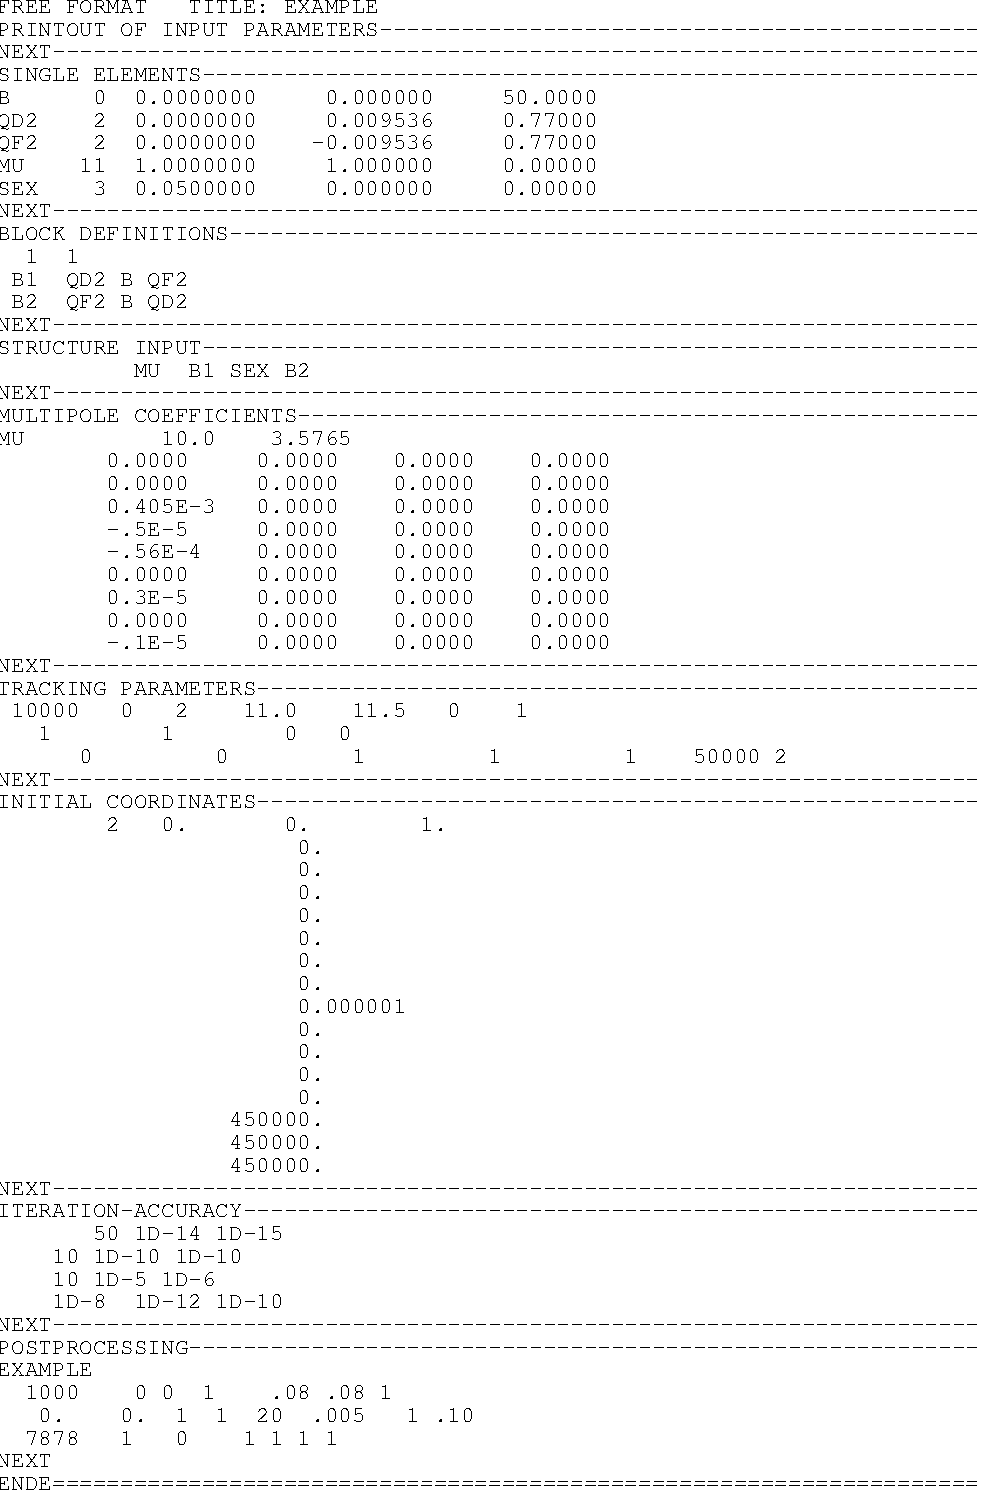
\includegraphics[height=14cm]{figures/expout1}
%     \end{center}
% \end{figure}

\clearpage

% ================================================================================================================================ %
\section{Output Example} \label{output}

The preprocessing part is shown first.

\begin{ctverbatim}
-----------------------------------------------------------------------------------------------------------------------------------

    OOOOOOOOOOOOOOOOOOOOO
    OO                 OO
    OO  PREPROCESSING  OO
    OO                 OO
    OOOOOOOOOOOOOOOOOOOOO

-----------------------------------------------------------------------------------------------------------------------------------


    STRUCTURE INPUT FILE HAS -THICK- LINEAR ELEMENTS


---- ENTRY CLORB ----/DPP= 0.00000 /CLOX/   0.00000   0.00000 /CLOY/   0.00000   0.00000 /ITERAT.=  2/ ACCURACY= 0.000000D+00
---- ENTRY CLORB ----/DPP= 0.00000 /CLOX/   0.00000   0.00000 /CLOY/   0.00000   0.00000 /ITERAT.=  2/ ACCURACY= 0.000000D+00
---- ENTRY CLORB ----/DPP= 0.00000 /CLOX/   0.00000   0.00000 /CLOY/   0.00000   0.00000 /ITERAT.=  2/ ACCURACY= 0.000000D+00
---- ENTRY CLORB ----/DPP= 0.00000 /CLOX/   0.00000   0.00000 /CLOY/   0.00000   0.00000 /ITERAT.=  2/ ACCURACY= 0.000000D+00

    Initial 4-D DA CLOSED ORBIT IN QMODDA (NO TUNE ADJUSTEMENT)
        0.000000000000000000000000000000000
        0.000000000000000000000000000000000
        0.000000000000000000000000000000000
        0.000000000000000000000000000000000

-----------------------------------------------------------------------------------------------------------------------------------
     DA INITIALIZATION: ORDER =  1, # of VARIABLES =  4, DIMENSION =  2


-----------------------------------------------------------------------------------------------------------------------------------
    ENTERING 4-D DA CLOSED ORBIT CALCULATION

---- closed orbit before correction----
 CLOX    0.00000000       0.00000000    
 CLOY    0.00000000       0.00000000    
---- after DA correction----
 CLOX    0.00000000       0.00000000    
 CLOY    0.00000000       0.00000000    
 ITERAT.=  1 ACCURACY= 0.000000D+00

SUCCESSFULL END OF 4-D DA CLOSED ORBIT CALCULATION IN ITERATION:    1

 CLOX    0.00000000       0.00000000    
  D-X    0.00000000       0.00000000    
 CLOY    0.00000000       0.00000000    
  D-Y    0.00000000       0.00000000    
 ITERAT.=  1 ACCURACY= 0.000000D+00


-----------------------------------------------------------------------------------------------------------------------------------
     DA INITIALIZATION: ORDER =  2, # of VARIABLES =  4, DIMENSION =  2

Check of the symplectic condition on the linear part
0.000000000000000       0.9999999999999998        0.000000000000000        0.000000000000000    
-0.9999999999999998        0.000000000000000        0.000000000000000        0.000000000000000    
0.000000000000000        0.000000000000000        0.000000000000000       0.9999999999999996    
0.000000000000000        0.000000000000000      -0.9999999999999996        0.000000000000000    
deviation for symplecticity   -3.3306690738754709E-014  %
0.12223867786724546       0.12223867786724549     

-----------------------------------------------------------------------------------------------------------------------------------

    TRACKING FOR CONSTANT MOMENTUM DEVIATION

          ------ NO ACCELERATION ------

                TUNE         CLO            CLOP              BET0           ALF0           GAMMA      

      X    0.1222386779   0.0000000       0.0000000        92.957545511    0.0000000000    0.010757599
                                                            0.000000000   -0.0000000000    0.000000000
      Y    0.1222386779   0.0000000       0.0000000       203.581213058   -0.0000000000    0.004912045
                                                            0.000000000   -0.0000000000    0.000000000


    REL. MOMENTUM DEVIATION= 0.0000000000000000
  ========================================

---- CLOSED ORBIT AND DECOUPLING (1=COU,0=DECOU)
/CLX /            0.000000000000000000000000000000000
/CLXP/            0.000000000000000000000000000000000
/CLY /            0.000000000000000000000000000000000
/CLYP/            0.000000000000000000000000000000000
/DCX /    1
/DCY /    1env
env
/IVER /   0
/IDFOR/   0
/ICLO6/   0
/ITION/   0
\end{ctverbatim}

% \begin{figure}[H]
% \begin{center}
%     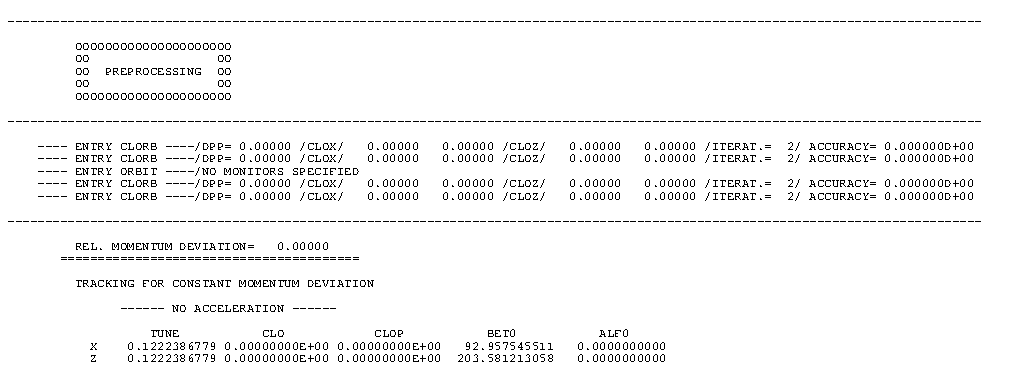
\includegraphics[width=16cm,height=13cm]{figures/expout2}
% \end{center}
% \end{figure}

\clearpage

Followed by the initial coordinates.

\begin{ctverbatim}
-----------------------------------------------------------------------------------------------------------------------------------

         OOOOOOOOOOOOOOOOOOOOOOOOOOO
         OO                       OO
         OO  INITIAL COORDINATES  OO
         OO                       OO
         OOOOOOOOOOOOOOOOOOOOOOOOOOO

-----------------------------------------------------------------------------------------------------------------------------------



     PARTICLE       3 RANDOM SEED        0 MOMENTUM DEVIATION   0.0000    


     ---- TWIN-TRAJECTORIES NO CL.ORBIT ADDED
     /X1  /           11.500000000000000000000000000000000
     /XP1 /           -0.000000000000000019769953827468216
     /Y1  /           17.018620942597696199527490534819663
     /YP1 /            0.000000000000000000000000000000000
     /SIG1/            0.000000000000000000000000000000000
     /DP1 /            0.000000000000000000000000000000000
     /X2  /           11.500000000000000000000000000000000
     /XP2 /            0.000000999999999980229994000959642
     /Y2  /           17.018620942597696199527490534819663
     /YP2 /            0.000000000000000000000000000000000
     /SIG2/            0.000000000000000000000000000000000
     /DP2 /            0.000000000000000000000000000000000


         UNCOUPLED AMPLITUDES AND EMITTANCES:
         AMPLITUDE-X =          11.500          AMPLITUDE-Y =          17.019  MM
         EMITTANCE-X =           1.423          EMITTANCE-Y =           1.423  PI*MRAD*MM

     ---- INITIAL COORD. OF TWIN-TRAJECTORIES
                     11.500000000000000000000000000000000
                     -0.000000000000000019769953827468216
                     17.018620942597696199527490534819663
                      0.000000000000000000000000000000000
                      0.000000000000000000000000000000000
                      0.000000000000000000000000000000000
                     11.500000000000000000000000000000000
                      0.000000999999999980229994000959642
                     17.018620942597696199527490534819663
                      0.000000000000000000000000000000000
                      0.000000000000000000000000000000000
                      0.000000000000000000000000000000000
                 450000.000000000000000000000000000000000
                 449999.999999999941792339086532592773438
                 449999.999999999941792339086532592773438

 
------------------------------------------------------------------------------------------------------------------------------------
 
  CALL TO CADCUM
 
 Machine length was    103.0800000000 [m]
\end{ctverbatim}

\clearpage

And the final coordinates for a regular (right side) and chaotic (left side) case.

\begin{ctverbatim}
-----------------------------------------------------------------------------------------------------------------------------------

         OOOOOOOOOOOOOOOO
         OO            OO
         OO  TRACKING  OO
         OO            OO
         OOOOOOOOOOOOOOOO

-----------------------------------------------------------------------------------------------------------------------------------


 
 Calling thck4d subroutine
 

     PARTICLE       1 AND       2 STABLE - RANDOM SEED        0 MOMENTUM DEVIATION   0.0000    
     REVOLUTION    10000

                      6.413505260046698630560513265663758
                     -0.089292907574702679029954310863104
                     -6.601359435036310507882717502070591
                      0.081356939205201914133702700837603
                      0.000000000000000000000000000000000
                      0.000000000000000000000000000000000
                      6.407742554197603190857535082614049
                     -0.089306143545032981578835062919097
                     -6.608681191308765967562521836953238
                      0.081353966356037088480945840274217
                      0.000000000000000000000000000000000
                      0.000000000000000000000000000000000
                 450000.000000000000000000000000000000000
                 449999.999999999941792339086532592773438
                 449999.999999999941792339086532592773438

     PARTICLE       3 AND       4 STABLE - RANDOM SEED        0 MOMENTUM DEVIATION   0.0000    
     REVOLUTION    10000

                     11.004259035154733581407526799011976
                     -0.017944489717545052120950543894651
                    -17.049149437508784643569015315733850
                      0.015505328739040841190544028904696
                      0.000000000000000000000000000000000
                      0.000000000000000000000000000000000
                     10.717352036206978738164252717979252
                     -0.079677127850136961195737228536018
                      5.973322092980881237167523067910224
                     -0.075407170859343758406723168263852
                      0.000000000000000000000000000000000
                      0.000000000000000000000000000000000
                 450000.000000000000000000000000000000000
                 449999.999999999941792339086532592773438
                 449999.999999999941792339086532592773438

-----------------------------------------------------------------------------------------------------------------------------------
\end{ctverbatim}

% \begin{figure}[H]
% \begin{center}
%     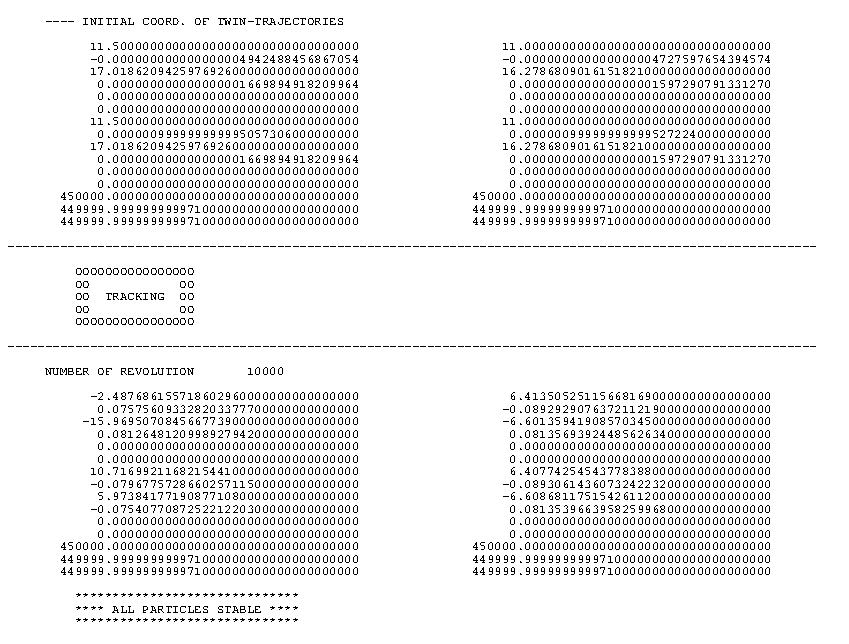
\includegraphics[width=16cm,height=13cm]{figures/expout3}
% \end{center}
% \end{figure}

\clearpage

Finally part of the post--processing for the two particle pairs are shown (chaotic on the left and regular on the right respectively) and a summary of the post--processing is given.

\begin{ctverbatim}

\end{ctverbatim}

% \begin{figure}[H]
% \begin{center}
%   \mbox{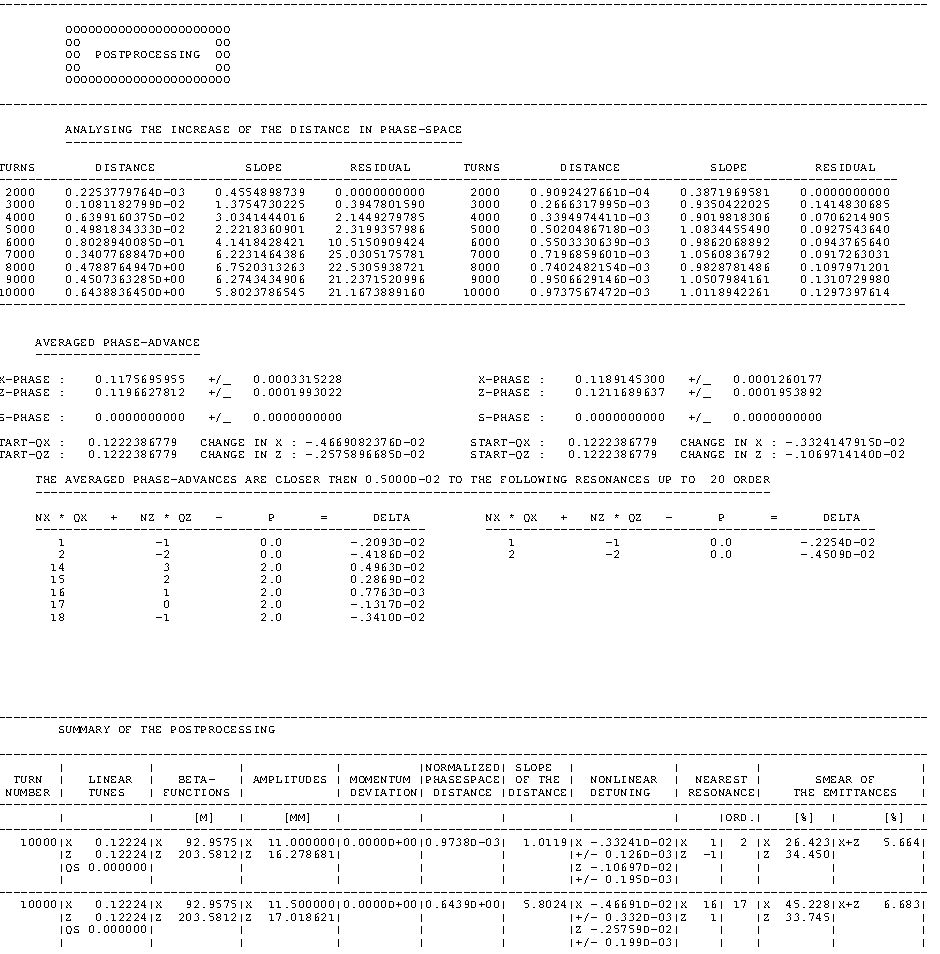
\includegraphics[width=16cm,height=21cm]{figures/expout4}}
% \end{center}
% \end{figure}

\clearpage

\section{Plot Example} \label{plots}

{\small In figure~\ref{Lya} a typical example of the evolution of the
  distance in phase space is shown of a regular and chaotic particle.
  Figure~\ref{H-proj} and figure~\ref{P-proj} show the corresponding
  horizontal phase space and the physical phase space projections
  respectively. An example of the stroboscoped phase space is shown in
  figure~\ref{P-stro}, where the motion in the chaotic case is beyond
  a ``separatrix'' in the four--dimensional phase space. Even in the
  FFT (figure~\ref{P-FFT}) one can see the effect of chaotic
  behaviour: it leads to a widening of the lines of the spectrum.}
\begin{figure}[H] \vspace*{-5mm}
\begin{center}
  \mbox{\includegraphics*[width=9.cm]{figures/exp1}}
  \\[5mm]
  \mbox{\includegraphics*[width=9.cm]{figures/exp9}}
 \caption{\small Evolution of the Distance of Phase Space for Regular
   \mbox{(upper part)} and Chaotic \mbox{(lower part)} Motion.}
 \label{Lya}
\end{center}
\end{figure} 

\begin{figure}[H]
\begin{center}
  \mbox{\includegraphics*[width=10.5cm]{figures/exp2}}
  \\[5mm]
  \mbox{\includegraphics*[width=10.5cm]{figures/exp10}}
 \caption{Horizontal Phase Space Projections for the
   Regular (upper part) and the Chaotic \mbox{(lower part)} Cases.}
 \label{H-proj}
\end{center}
\end{figure}

\begin{figure}[H]
\begin{center}
  \mbox{\includegraphics*[width=10.5cm]{figures/exp4}}
  \\[5mm]
  \mbox{\includegraphics*[width=10.5cm]{figures/exp12}}
 \caption{Physical Phase Space Projections for the Regular
   \mbox{(upper part)} and the Chaotic \mbox{(lower part)} Cases.}
 \label{P-proj}
\end{center}
\end{figure}

\begin{figure}[H]
\begin{center}
  \mbox{\includegraphics*[width=10.5cm]{figures/exp6}}
  \\[5mm]
  \mbox{\includegraphics*[width=10.5cm]{figures/exp14}}
 \caption{\small{Stroboscoped Vertical Phase Space Projections
     for the Regular (upper part) and the Chaotic (lower part) Cases
     respectively.  The regular motion stays inside a ``separatrix''
     with two unstable fix--points visible, while the chaotic motion
     is clearly outside this ``separatrix''.}}
 \label{P-stro}
\end{center}
\end{figure}

\begin{figure}[H]
\begin{center}
  \mbox{\includegraphics*[width=10.5cm]{figures/exp7}}
  \\[5mm]
  \mbox{\includegraphics*[width=10.5cm]{figures/exp15}}
 \caption{Horizontal FFT--Analysis for the Regular (upper part)
   and the Chaotic (lower part) Cases.}
 \label{P-FFT}
\end{center}
\end{figure}

% \cleardoublepage

\backmatter
\begin{thebibliography}{99}
    %
    \bibitem{DALIE}
        LBL diffential algebra package and LieLib routines courtesy of \'{E}.~Forest.
    %
    \bibitem{Ripken95}
        G.~Ripken and F.~Schmidt,
        ``A symplectic six-dimensional thin-lens formalism for tracking'',
        CERN SL 95--12 (AP)(1995), DESY 95--063 (1995);\\
        G.~Ripken and F.~Schmidt,
        ``Construction of Nonlinear Symplectic Six-Dimensional Thin-Lens Maps by Exponentiation'',
        DESY 95--189 (1995), \url{http://cern.ch/Frank.Schmidt/report/ripken2.pdf};\\
        D.P.~Barber, K.~Heinemann, G.~Ripken and F.~Schmidt,
        ``Symplectic Thin\,-\,Lens Transfer Maps for SixTrack: Treatment of  Bending Magnets in Terms of the Exact Hamiltonian'',
        DESY 96--156 (1995), \url{http://cern.ch/Frank.Schmidt/report/ripken3.pdf}.
    %
    \bibitem{RACETRACK}
        A.~Wrulich,
        ``RACETRACK, A computer code for the simulation of nonlinear motion in accelerators'',
        DESY 84--026 (1984).
    %
    \bibitem{FASTRAC}
        B.~Leemann and \'{E}.~Forest,
        ``Brief description of the tracking codes FASTRAC and THINTRAC'',
        SSC Note SSC--133.
    %
    \bibitem{Ripken85}
        G.~Ripken,
        ``Nonlinear canonical equations of coupled synchro-betatron motion and their solution within the framework of a nonlinear 6-dimensional (symplectic) tracking program for ultra-relativistic protons'',
        DESY 85--084 (1985).
    %
    \bibitem{Ripken87}
        D.P.~Barber, G.~Ripken and F.~Schmidt,
        ``A nonlinear canonical formalism for the coupled synchro-betatron motion of protons with arbitrary energy'',
        DESY 87--036 (1987);\\
        G.~Ripken and F.~Schmidt,
        ``A symplectic six-dimensional thin-lens formalism for tracking'',
        CERN/SL/95--12 (AP), DESY 95--063 (1995), \url{http://cern.ch/Frank.Schmidt/report/ripken.pdf};
        %K.~Heinemann,
    %
    \bibitem{HBOOK}
        R.~Brun and D.~Lienart,
        ``HBOOK User Guide'',
        CERN Program Library Y250 (1987).
    %
    \bibitem{HPLOT}
        R.~Brun and N.C.~Somon,
        ``HPLOT User Guide'',
        CERN Program Library Y251 (1988).
    %
    \bibitem{HIGZ}
        R.~Bock, R.~Brun, O.~Couet, N.C.~Somon, C.E. Vandoni and P. Zanarini,
        ``HIGZ User Guide'',
        CERN Program Library Q120.
    %
    \bibitem{Gilbert78}
        G.~Guignard,
        ``A general treatment of resonances in accelerators'',
        CERN 78--11 (1978).
    %
    \bibitem{Berz89}
        M.~Berz,
        ``Differential algebra description of beam dynamics to very high orders'',
        Particle Accelerators, 1989, Vol. \underline{24}, pp. 109--124.
    %
    \bibitem{DAFOR}
        M.~Berz,
        ``DAFOR -- Differential Algebra Precompiler Version 3, Reference Manual'',
        MSUCL--755 (1991).
    %
    \bibitem{Sixvec}
        F.~Schmidt and M.~Vaenttinen,
        ``Vectorisation of the single particle tracking program SixTrack'',
        CERN SL Note 90--20 (1990) (AP).
    %
    \bibitem{thesis}
        F.~Schmidt,
        ``Untersuchungen zur dynamischen Akzeptanz von Protonenbeschleunigern und ihre Begrenzung durch chaotische Bewegung'',
        DESY HERA 88--02, (1988).
    %
    %\bibitem{Daspeed} J.~Irwin, private communication.
    %
    \bibitem{CONVERTOR}
        H.~Grote,
        ``A MAD--SixTrack interface'',
        SL Note 97--02 (AP).
    %
    \bibitem{sixphys}
        SixTrack Physics Manual,
        \url{http://sixtrack.web.cern.ch/SixTrack/}
    %
    \bibitem{h5_doc}
        HDF5 Software Documentation,
        \url{https://support.hdfgroup.org/HDF5/doc/H}
    %
    \bibitem{Forest89}
        M.~Berz, \'{E}. Forest and J. Irwin,
        ``Normal form methods for complicated periodic systems: a complete solution using differential algebra and lie operators'',
        Particle Accelerators, 1989, Vol. \underline{24}, pp. 91--107.
    %
    \bibitem{BasErs}
        M.~Bassetti and G.A.~Erskine,
        ``Closed expression for the electrical field of a two-dimensional Gaussian charge'',
        CERN--ISR--TH/80--06.
    %
    \bibitem{Hirata}
        K.~Hirata, H.~Moshammer, F.~Ruggiero and M.~Bassetti,
        ``Synchro-Beam interaction'',
        CERN SL-AP/90-02 (1990) and Proc. Workshop on Beam Dynamics Issues of High-Luminosity Asymmetric Collider Rings, Berkeley, 1990, ed. A.M. Sessler (AIP Conf. Proc. 214, New York, 1990), pp. 389-404;\\
        K.~Hirata, H.~Moshammer and F.~Ruggiero,
        ``A symplectic beam-beam interaction with energy change'',
        KEK preprint 92-117 A (1992) and Part. Accel. 40, 205-228 (1993);\\
        K.~Hirata,
        ``BBC User's Guide; A Computer Code for Beam-Beam Interaction with a Crossing Angle, version 3.4'',
        SL-Note 97-57 AP.
    %
    \bibitem{ripbeam}
        L.H.A.~Leunissen, F.~Schmidt and G.~Ripken,
        ``6D Beam--Beam Kick including Coupled Motion'',
        LHC Project Report 369, \url{http://cern.ch/Frank.Schmidt/report/ripken\_new.pdf}.
    %
    \bibitem{SODD}
        F.~Schmidt,
        ``SODD: A Computer Code to calculate Detuning and Distortion Function Terms in First and Second Order'',
        CERN SL/Note 99--009 (AP), \url{http://cern.ch/Frank.Schmidt/report/sodd\_manual.pdf}
    %
    \bibitem{MAD}
        H.~Grote and F.C.~Iselin,
        ``The MAD program (Methodical Accelerator Design), Version 8.10, User's Reference Manual'',
        CERN SL 90--13 (AP) (Rev. 4), \url{http://cern.ch/Hans.Grote/mad/mad8/doc/mad8\_user.ps.gz}.
    %
    \bibitem{dipedge}
        R.~Molloy and S.~Blitz,
        ``Fringe Field Effects on Bending Magnets, Derived for, TRANSPORT/TURTLE'',
        FERMILAB-TM-2564-AD-APC-PPD, \url{http://lss.fnal.gov/archive/test-tm/2000/fermilab-tm-2564-ad-apc-ppd.pdf}
    %
    \bibitem{ERIC} private communication. % with whom?
    %
    \bibitem{RANECU}
        F.~James,
        ``A Review of Pseudorandom Number Generators'',
        CERN DD/ 88/22, 1988.
        % F.~James,
        % ``A review of pseudo-random number generators'',
        % to be published in Computer Physics Communication.
    %
    \bibitem{Auti}
        B.~Autin and Y.~Marti,
        ``Closed Orbit Correction of A.G. Machines Using a Small Number of Magnets'',
        CERN--ISR--MA/73--17.
    %
    \bibitem{Massimo}
        M.~Giovannozzi,
        ``Description of software tools to perform tune-shift correction using normal forms'',
        CERN SL Note 93--111 (AP).
    %
    \bibitem{Refine}
        F.~Schmidt, F.~Willeke and F.~Zimmermann,
        ``Comparison of methods to determine long-term stability in proton storage rings'',
        1991, Particle Accelerators, Vol. \underline{35}, pp. 249--256.
    %
    \bibitem{plato1}
        R.~Bartolini, A.~Bazzani, M.~Giovannozzi, W.~Scandale, E.~Todesco,
        ``Tune evaluation in simulations and experiments'',
        Part. Accel. 52 147
    %
    \bibitem{plato2}
        M.~Giovannozzi, E.~Todesco, A.~Bazzani and R.~Bartolini (1997),
        ``PLATO: a program library for the analysis of nonlinear betatronic motion'',
        Nucl. Instrum. and Methods A 388 1
    %
    \bibitem{NAFFpaper}
        J.~Laskar, C.~Froeschle and C.~Celletti,
        ``The measure of chaos by the numerical analysis of the fundamental frequencies. Application to the standard mapping'',
        Physica D, vol. 56, pp 253-269, 1992.
    %
    \bibitem{NAFFpaper2}
        S.~Kostoglou, N.~Karastathis, Y.~Papaphilippou, D.~Pellegrini and P.~Zisopoulos,
        ``Development of computational tools for noise studies in the LHC'',
        2017, Proceedings of IPAC'17, Copenhagen, Denmark, 2017.
    %
    \bibitem{sixbuild}
        SixTrack build manual, see SixTrack website, \url{http://sixtrack.web.cern.ch/SixTrack/}
    %
    \bibitem{sixdesk1}
        SixDesk manual, see SixTrack website, \url{http://sixtrack.web.cern.ch/SixTrack/}
    %
    \bibitem{sixdesk2}
        SixDesk manual, \url{https://www.overleaf.com/1345694dwypbp#/3325092/}
    %
    % \bibitem{PATRAC}
    %     A.~Hilaire and A.~Warman,
    %     ``A program for single particle tracking'',
    %     CERN SPS/88--8 (AMS).
    %
    \bibitem{RFmultsPaper}
        J.~B.~Garcia et al.,
        ``Long term dynamics of the high luminosity Large Hadron Collider with crab cavities'',
        2016, PHYSICAL REVIEW ACCELERATORS AND BEAMS 19, 101003 (2016).
    %
    \bibitem{DYNKpaper}
        K.~Sjobak, H.~Burkhardt, R.D.~Maria, A.~Mereghetti and A.~Santamaria,
        ``General functionality for turn-dependent element properties in SixTrack'',
        2015, Procedings of IPAC'13, Richmond, VA, USA, May 2015.
    %
    \bibitem{DYNKpaper2}
        K.~Sjobak, V.K.~Berglyd~Olsen, R.~De~Maria, M.~Fitterer, A.~Santamaría~García, H. Garcia-Morales, A.~Mereghetti, J.F.~Wagner, S.J.~Wretborn,
        ``Dynamic simulations in SixTrack'',
        CERN
    %
    \bibitem{SRussen:fieldComp}
        S.~Russenschuck,
        ``Field computation for Accelerator Magnets'',
        Wiley-VCH, 2010
    %
    \bibitem{BurlaKing:CurrentRamp}
        P.~Burla, Q.~King and J.G.~Pett,
        ``Optimisation of the current ramp for the LHC'',
        Proceedings of the 1999 Particle Accelerator Conference, New York, 1999.
    %
    \bibitem{collimat:trenkler}
        T.~Trenkler, J.B.~Jeanneret,
        ``K2, A software package evaluating collimation systems in circular colliders (manual)'',
        CERN SL/94–105 (AP), 1994.
    %
    \bibitem{collimat:robert_demolaize}
        G.~Robert-Demolaize, R.~Assmann, S.~Redaelli, F.~Schmidt,
        ``A new version of SixtTrack with collimation and aperture interface'',
        CERN, Geneva, Switzerland (PAC 2005).
    %
    \bibitem{collimat:assmann}
        R.~Assmann, J.B.~Jeanneret, D.~Kaltchev,
        ``Status of Robustness Studies for the LHC Collimation'',
        APAC 2001.
    %
    \bibitem{pythia8}
        T.~Sjöstrand, S.~Mrenna, P.~Skands,
        ``A Brief Introduction to PYTHIA 8.1 '',
        Comput. Phys. Comm. 178 (2008) 852 [arXiv:0710.3820].
    %
    \bibitem{pythia_phys}
        T.~Sjöstrand, S.~Mrenna, P.~Skands,
        ``PYTHIA 6.4 Physics and Manual'',
        JHEP05 (2006) 026.
    %
    \bibitem{coupling:1}
        V.~Vlachoudis {\it et al.}, ``Status of Fluka coupling to Sixtrack'',
        Proceedings of Tracking for Collimation Workshop (WP5), CERN, Geneva,
        Switzerland (in publication).
    %
    \bibitem{coupling:2}
        A.~Mereghetti, Performance Evaluation of the SPS Scraping System
        in View of the High Luminosity LHC, Ph.~D.~thesis, UniMAN, Manchester,
        UK (2015).
    %
    \bibitem{ffield:1}
        B. Dalena \emph{et al.}, ``Fringe Field Modeling for the High Luminosity LHC Large Aperture quadrupole'',
        Proceedings of IPAC’14, Dresden, Germany, June 2014, paper TUPRO002, pp.~993--996.
    %
    \bibitem{ffield:2}
        T. Pugnat \emph{et al.}, ``Accurate and Efficient Tracking in Electromagnetic Quadrupoles'',
        Proceedings of IPAC’18, Vancouver, Canada, June 2014, paper THPAK004, pp.~3207.
    %
    \bibitem{ffield:3}
        A. Simona \emph{et al.}, ``High order time integrators for the simulation of charged particle motion in magnetic quadrupoles'',
        Elsevier, February 2019.
    %
    \bibitem{cheby:1}
        G. Stancari, ``Calculation of the transverse kicks generated by the bends of a hollow electron lens'',
        FERMILAB-FN-0972-APC, FermiLab, Batavia, Illinois, USA (2014).
    %
    \bibitem{ranlux}
        F. James, ``RANLUX: A FORTRAN Implementation of the High Quality Pseudorandom Number Generator of Luscher''.
        Comput.Phys.Commun. 79 (1994): 111–14.DOI:10.1016/0010-4655(94)90233-X.
    %
    \bibitem{ranecu1}
        F. James, ``A Review of Pseudorandom Number Generators'',
        Computer Physics Communications 60, no. 3 (1 October 1990): 329–44. DOI:10.1016/0010-4655(90)90032-V.
    %
    \bibitem{ranecu2}
        P. L’Ecuyer, ``Efficient and Portable Combined Random Number Generators'',
        Commun. ACM 31, no. 6 (June 1988): 742–751. DOI:10.1145/62959.62969.
    %
    \bibitem{crystal:1}
    V.~Previtali, ``Performance Evaluation of a Crystal-enhanced Collimation System for the LHC'',
    Ph.~D.~thesis, EPFL, Lausanne, Switzerland (2010).
    %
    \bibitem{crystal:2}
    D.~Mirarchi, ``Crystal collimation for LHC'',
    Ph.~D.~thesis, Imperial College, London, UK (2015).
    %
    \bibitem{crystal:3}
    D.~Mirarchi \emph{et al.}, ``A crystal routine for collimation studies in circular proton accelerators'',
    Proceedings of the 6$^{\mathrm th}$ International Conference Channeling: ``Charged \& Neutral Particles Channeling Phenomena'', Capri, Italy (2014).
    %
    \bibitem{crystal:4}
    D.~Mirarchi \emph{et al.}, ``Crystal implementation in SixTrack for proton beams'',
    ICFA Mini-Workshop on Tracking for Collimation in Particle Accelerators, CERN, Geneva, Switzerland (2015).
    %
    \bibitem{crystal:5}
    F.~Forcher, ``An improved simulation routine for modelling coherent high-energy proton interactions with bent crystals'',
    Bachelor~thesis, UniPD, Padova, Italy (2017).
    %
    \bibitem{crystal:6}
    R.~Rossi, ``Experimental Assessment of Crystal Collimation at the Large Hadron Collider'',
    Ph.~D.~thesis, Universit\`a La Sapienza, Roma, Italy (2018).
    %
    \addcontentsline{toc}{chapter}{Bibliography}
\end{thebibliography}

\cleardoublepage

\pdfbookmark{Keyword Index}{Index}
\printindex
\cleardoublepage

\pdfbookmark{List of Tables}{List of Tables}
\listoftables
\cleardoublepage

\end{document}
